\documentclass[twoside]{book}

% Packages required by doxygen
\usepackage{calc}
\usepackage{doxygen}
\usepackage{graphicx}
\usepackage[utf8]{inputenc}
\usepackage{makeidx}
\usepackage{multicol}
\usepackage{multirow}
\usepackage{textcomp}
\usepackage[table]{xcolor}

% Font selection
\usepackage[T1]{fontenc}
\usepackage{mathptmx}
\usepackage[scaled=.90]{helvet}
\usepackage{courier}
\usepackage{amssymb}
\usepackage{sectsty}
\renewcommand{\familydefault}{\sfdefault}
\allsectionsfont{%
  \fontseries{bc}\selectfont%
  \color{darkgray}%
}
\renewcommand{\DoxyLabelFont}{%
  \fontseries{bc}\selectfont%
  \color{darkgray}%
}

% Page & text layout
\usepackage{geometry}
\geometry{%
  a4paper,%
  top=2.5cm,%
  bottom=2.5cm,%
  left=2.5cm,%
  right=2.5cm%
}
\tolerance=750
\hfuzz=15pt
\hbadness=750
\setlength{\emergencystretch}{15pt}
\setlength{\parindent}{0cm}
\setlength{\parskip}{0.2cm}
\makeatletter
\renewcommand{\paragraph}{%
  \@startsection{paragraph}{4}{0ex}{-1.0ex}{1.0ex}{%
    \normalfont\normalsize\bfseries\SS@parafont%
  }%
}
\renewcommand{\subparagraph}{%
  \@startsection{subparagraph}{5}{0ex}{-1.0ex}{1.0ex}{%
    \normalfont\normalsize\bfseries\SS@subparafont%
  }%
}
\makeatother

% Headers & footers
\usepackage{fancyhdr}
\pagestyle{fancyplain}
\fancyhead[LE]{\fancyplain{}{\bfseries\thepage}}
\fancyhead[CE]{\fancyplain{}{}}
\fancyhead[RE]{\fancyplain{}{\bfseries\leftmark}}
\fancyhead[LO]{\fancyplain{}{\bfseries\rightmark}}
\fancyhead[CO]{\fancyplain{}{}}
\fancyhead[RO]{\fancyplain{}{\bfseries\thepage}}
\fancyfoot[LE]{\fancyplain{}{}}
\fancyfoot[CE]{\fancyplain{}{}}
\fancyfoot[RE]{\fancyplain{}{\bfseries\scriptsize Generated on Fri Apr 10 2015 20\-:55\-:16 for Mixage -\/ T\-P13 by Doxygen }}
\fancyfoot[LO]{\fancyplain{}{\bfseries\scriptsize Generated on Fri Apr 10 2015 20\-:55\-:16 for Mixage -\/ T\-P13 by Doxygen }}
\fancyfoot[CO]{\fancyplain{}{}}
\fancyfoot[RO]{\fancyplain{}{}}
\renewcommand{\footrulewidth}{0.4pt}
\renewcommand{\chaptermark}[1]{%
  \markboth{#1}{}%
}
\renewcommand{\sectionmark}[1]{%
  \markright{\thesection\ #1}%
}

% Indices & bibliography
\usepackage{natbib}
\usepackage[titles]{tocloft}
\setcounter{tocdepth}{3}
\setcounter{secnumdepth}{5}
\makeindex

% Hyperlinks (required, but should be loaded last)
\usepackage{ifpdf}
\ifpdf
  \usepackage[pdftex,pagebackref=true]{hyperref}
\else
  \usepackage[ps2pdf,pagebackref=true]{hyperref}
\fi
\hypersetup{%
  colorlinks=true,%
  linkcolor=blue,%
  citecolor=blue,%
  unicode%
}

% Custom commands
\newcommand{\clearemptydoublepage}{%
  \newpage{\pagestyle{empty}\cleardoublepage}%
}


%===== C O N T E N T S =====

\begin{document}

% Titlepage & ToC
\hypersetup{pageanchor=false}
\pagenumbering{roman}
\begin{titlepage}
\vspace*{7cm}
\begin{center}%
{\Large Mixage -\/ T\-P13 }\\
\vspace*{1cm}
{\large Generated by Doxygen 1.8.6}\\
\vspace*{0.5cm}
{\small Fri Apr 10 2015 20:55:16}\\
\end{center}
\end{titlepage}
\clearemptydoublepage
\tableofcontents
\clearemptydoublepage
\pagenumbering{arabic}
\hypersetup{pageanchor=true}

%--- Begin generated contents ---
\chapter{Namespace Index}
\section{Namespace List}
Here is a list of all namespaces with brief descriptions\-:\begin{DoxyCompactList}
\item\contentsline{section}{\hyperlink{namespaceMixageSonore}{Mixage\-Sonore} }{\pageref{namespaceMixageSonore}}{}
\end{DoxyCompactList}

\chapter{Hierarchical Index}
\section{Class Hierarchy}
This inheritance list is sorted roughly, but not completely, alphabetically\-:\begin{DoxyCompactList}
\item \contentsline{section}{composant}{\pageref{classcomposant}}{}
\begin{DoxyCompactList}
\item \contentsline{section}{consommateur}{\pageref{classconsommateur}}{}
\begin{DoxyCompactList}
\item \contentsline{section}{consommateur\-\_\-base}{\pageref{classconsommateur__base}}{}
\begin{DoxyCompactList}
\item \contentsline{section}{filtre\-\_\-base}{\pageref{classfiltre__base}}{}
\begin{DoxyCompactList}
\item \contentsline{section}{filtre\-\_\-compose}{\pageref{classfiltre__compose}}{}
\begin{DoxyCompactList}
\item \contentsline{section}{mixer\-\_\-element}{\pageref{classmixer__element}}{}
\item \contentsline{section}{mixeur}{\pageref{classmixeur}}{}
\item \contentsline{section}{volume\-\_\-compose}{\pageref{classvolume__compose}}{}
\end{DoxyCompactList}
\item \contentsline{section}{multiplicateur}{\pageref{classmultiplicateur}}{}
\item \contentsline{section}{operation\-\_\-binaire$<$ T $>$}{\pageref{classoperation__binaire}}{}
\item \contentsline{section}{volume}{\pageref{classvolume}}{}
\end{DoxyCompactList}
\end{DoxyCompactList}
\item \contentsline{section}{enregistreur\-\_\-fichier}{\pageref{classenregistreur__fichier}}{}
\item \contentsline{section}{enregistreur\-\_\-fichier\-\_\-texte}{\pageref{classenregistreur__fichier__texte}}{}
\item \contentsline{section}{filtre}{\pageref{classfiltre}}{}
\begin{DoxyCompactList}
\item \contentsline{section}{filtre\-\_\-base}{\pageref{classfiltre__base}}{}
\end{DoxyCompactList}
\end{DoxyCompactList}
\item \contentsline{section}{producteur}{\pageref{classproducteur}}{}
\begin{DoxyCompactList}
\item \contentsline{section}{filtre}{\pageref{classfiltre}}{}
\item \contentsline{section}{producteur\-\_\-base}{\pageref{classproducteur__base}}{}
\begin{DoxyCompactList}
\item \contentsline{section}{file\-\_\-reader}{\pageref{classfile__reader}}{}
\item \contentsline{section}{filtre\-\_\-base}{\pageref{classfiltre__base}}{}
\item \contentsline{section}{harmonique}{\pageref{classharmonique}}{}
\item \contentsline{section}{signal\-\_\-constant}{\pageref{classsignal__constant}}{}
\end{DoxyCompactList}
\end{DoxyCompactList}
\end{DoxyCompactList}
\item \contentsline{section}{counted\-\_\-ptr$<$ T $>$}{\pageref{classcounted__ptr}}{}
\item exception\begin{DoxyCompactList}
\item \contentsline{section}{composant\-\_\-exception}{\pageref{classcomposant__exception}}{}
\end{DoxyCompactList}
\item \contentsline{section}{flot}{\pageref{classflot}}{}
\begin{DoxyCompactList}
\item \contentsline{section}{imp\-\_\-flot}{\pageref{classimp__flot}}{}
\end{DoxyCompactList}
\end{DoxyCompactList}

\chapter{Class Index}
\section{Class List}
Here are the classes, structs, unions and interfaces with brief descriptions\-:\begin{DoxyCompactList}
\item\contentsline{section}{\hyperlink{classcomposant}{composant} \\*Interface d'un composant du systeme sonore }{\pageref{classcomposant}}{}
\item\contentsline{section}{\hyperlink{classcomposant__exception}{composant\-\_\-exception} \\*Classe qui gère les exceptions liées à un composant }{\pageref{classcomposant__exception}}{}
\item\contentsline{section}{\hyperlink{classconsommateur}{consommateur} \\*Interface d'un consommateur d'échantillons sonores. Il s'agit d'une interface décrivant un composant qui ne possède que des entrées }{\pageref{classconsommateur}}{}
\item\contentsline{section}{\hyperlink{classconsommateur__base}{consommateur\-\_\-base} }{\pageref{classconsommateur__base}}{}
\item\contentsline{section}{\hyperlink{classcounted__ptr}{counted\-\_\-ptr$<$ T $>$} \\*Classe gérant un \char`\"{}smart pointer\char`\"{} }{\pageref{classcounted__ptr}}{}
\item\contentsline{section}{\hyperlink{classenregistreur__fichier}{enregistreur\-\_\-fichier} \\*Un consommateur qui enregistre ses entrées dans un fichier binaire ; 44100 Hz, 16bits signé, entrelacé }{\pageref{classenregistreur__fichier}}{}
\item\contentsline{section}{\hyperlink{classenregistreur__fichier__texte}{enregistreur\-\_\-fichier\-\_\-texte} \\*Un consommateur qui enregistre ses entrées dans un fichier texte ; une ligne = un échantillon de chaque canal }{\pageref{classenregistreur__fichier__texte}}{}
\item\contentsline{section}{\hyperlink{classfile__reader}{file\-\_\-reader} }{\pageref{classfile__reader}}{}
\item\contentsline{section}{\hyperlink{classfiltre}{filtre} \\*Interface associée à un filtre sonore. Ce filtre est considéré comme un producteur / consommateur d'échantillons sonores. Il possède donc des entrées et des sorties }{\pageref{classfiltre}}{}
\item\contentsline{section}{\hyperlink{classfiltre__base}{filtre\-\_\-base} }{\pageref{classfiltre__base}}{}
\item\contentsline{section}{\hyperlink{classfiltre__compose}{filtre\-\_\-compose} }{\pageref{classfiltre__compose}}{}
\item\contentsline{section}{\hyperlink{classflot}{flot} \\*Interface associee a un flot de donnees reliant deux composants du systeme }{\pageref{classflot}}{}
\item\contentsline{section}{\hyperlink{classharmonique}{harmonique} }{\pageref{classharmonique}}{}
\item\contentsline{section}{\hyperlink{classimp__flot}{imp\-\_\-flot} }{\pageref{classimp__flot}}{}
\item\contentsline{section}{\hyperlink{classmixer__element}{mixer\-\_\-element} }{\pageref{classmixer__element}}{}
\item\contentsline{section}{\hyperlink{classmixeur}{mixeur} }{\pageref{classmixeur}}{}
\item\contentsline{section}{\hyperlink{classmultiplicateur}{multiplicateur} }{\pageref{classmultiplicateur}}{}
\item\contentsline{section}{\hyperlink{classoperation__binaire}{operation\-\_\-binaire$<$ T $>$} }{\pageref{classoperation__binaire}}{}
\item\contentsline{section}{\hyperlink{classproducteur}{producteur} \\*Interface d'un producteur d'échantillons sonores. Il s'agit d'une interface décrivant un composant ne possédant que des sorties }{\pageref{classproducteur}}{}
\item\contentsline{section}{\hyperlink{classproducteur__base}{producteur\-\_\-base} }{\pageref{classproducteur__base}}{}
\item\contentsline{section}{\hyperlink{classsignal__constant}{signal\-\_\-constant} }{\pageref{classsignal__constant}}{}
\item\contentsline{section}{\hyperlink{classvolume}{volume} }{\pageref{classvolume}}{}
\item\contentsline{section}{\hyperlink{classvolume__compose}{volume\-\_\-compose} }{\pageref{classvolume__compose}}{}
\end{DoxyCompactList}

\chapter{File Index}
\section{File List}
Here is a list of all files with brief descriptions\-:\begin{DoxyCompactList}
\item\contentsline{section}{include/\hyperlink{composant_8h}{composant.\-h} }{\pageref{composant_8h}}{}
\item\contentsline{section}{include/\hyperlink{composant__exception_8h}{composant\-\_\-exception.\-h} }{\pageref{composant__exception_8h}}{}
\item\contentsline{section}{include/\hyperlink{consommateur_8h}{consommateur.\-h} }{\pageref{consommateur_8h}}{}
\item\contentsline{section}{include/\hyperlink{constantes_8h}{constantes.\-h} }{\pageref{constantes_8h}}{}
\item\contentsline{section}{include/\hyperlink{counted__ptr_8h}{counted\-\_\-ptr.\-h} }{\pageref{counted__ptr_8h}}{}
\item\contentsline{section}{include/\hyperlink{enregistreur__fichier_8h}{enregistreur\-\_\-fichier.\-h} }{\pageref{enregistreur__fichier_8h}}{}
\item\contentsline{section}{include/\hyperlink{enregistreur__fichier__texte_8h}{enregistreur\-\_\-fichier\-\_\-texte.\-h} }{\pageref{enregistreur__fichier__texte_8h}}{}
\item\contentsline{section}{include/\hyperlink{filtre_8h}{filtre.\-h} }{\pageref{filtre_8h}}{}
\item\contentsline{section}{include/\hyperlink{flot_8h}{flot.\-h} }{\pageref{flot_8h}}{}
\item\contentsline{section}{include/\hyperlink{producteur_8h}{producteur.\-h} }{\pageref{producteur_8h}}{}
\item\contentsline{section}{src/\hyperlink{consommateur__base_8cpp}{consommateur\-\_\-base.\-cpp} }{\pageref{consommateur__base_8cpp}}{}
\item\contentsline{section}{src/\hyperlink{consommateur__base_8h}{consommateur\-\_\-base.\-h} }{\pageref{consommateur__base_8h}}{}
\item\contentsline{section}{src/\hyperlink{file__reader_8cpp}{file\-\_\-reader.\-cpp} }{\pageref{file__reader_8cpp}}{}
\item\contentsline{section}{src/\hyperlink{file__reader_8h}{file\-\_\-reader.\-h} }{\pageref{file__reader_8h}}{}
\item\contentsline{section}{src/\hyperlink{filtre__base_8cpp}{filtre\-\_\-base.\-cpp} }{\pageref{filtre__base_8cpp}}{}
\item\contentsline{section}{src/\hyperlink{filtre__base_8h}{filtre\-\_\-base.\-h} }{\pageref{filtre__base_8h}}{}
\item\contentsline{section}{src/\hyperlink{filtre__compose_8cpp}{filtre\-\_\-compose.\-cpp} }{\pageref{filtre__compose_8cpp}}{}
\item\contentsline{section}{src/\hyperlink{filtre__compose_8h}{filtre\-\_\-compose.\-h} }{\pageref{filtre__compose_8h}}{}
\item\contentsline{section}{src/\hyperlink{harmonique_8cpp}{harmonique.\-cpp} }{\pageref{harmonique_8cpp}}{}
\item\contentsline{section}{src/\hyperlink{harmonique_8h}{harmonique.\-h} }{\pageref{harmonique_8h}}{}
\item\contentsline{section}{src/\hyperlink{imp__flot_8cpp}{imp\-\_\-flot.\-cpp} }{\pageref{imp__flot_8cpp}}{}
\item\contentsline{section}{src/\hyperlink{imp__flot_8h}{imp\-\_\-flot.\-h} }{\pageref{imp__flot_8h}}{}
\item\contentsline{section}{src/\hyperlink{main_8cpp}{main.\-cpp} }{\pageref{main_8cpp}}{}
\item\contentsline{section}{src/\hyperlink{mixer__element_8cpp}{mixer\-\_\-element.\-cpp} }{\pageref{mixer__element_8cpp}}{}
\item\contentsline{section}{src/\hyperlink{mixer__element_8h}{mixer\-\_\-element.\-h} }{\pageref{mixer__element_8h}}{}
\item\contentsline{section}{src/\hyperlink{mixeur_8cpp}{mixeur.\-cpp} }{\pageref{mixeur_8cpp}}{}
\item\contentsline{section}{src/\hyperlink{mixeur_8h}{mixeur.\-h} }{\pageref{mixeur_8h}}{}
\item\contentsline{section}{src/\hyperlink{multiplicateur_8cpp}{multiplicateur.\-cpp} }{\pageref{multiplicateur_8cpp}}{}
\item\contentsline{section}{src/\hyperlink{multiplicateur_8h}{multiplicateur.\-h} }{\pageref{multiplicateur_8h}}{}
\item\contentsline{section}{src/\hyperlink{operation__binaire_8h}{operation\-\_\-binaire.\-h} }{\pageref{operation__binaire_8h}}{}
\item\contentsline{section}{src/\hyperlink{producteur__base_8cpp}{producteur\-\_\-base.\-cpp} }{\pageref{producteur__base_8cpp}}{}
\item\contentsline{section}{src/\hyperlink{producteur__base_8h}{producteur\-\_\-base.\-h} }{\pageref{producteur__base_8h}}{}
\item\contentsline{section}{src/\hyperlink{signal__constant_8cpp}{signal\-\_\-constant.\-cpp} }{\pageref{signal__constant_8cpp}}{}
\item\contentsline{section}{src/\hyperlink{signal__constant_8h}{signal\-\_\-constant.\-h} }{\pageref{signal__constant_8h}}{}
\item\contentsline{section}{src/\hyperlink{volume_8cpp}{volume.\-cpp} }{\pageref{volume_8cpp}}{}
\item\contentsline{section}{src/\hyperlink{volume_8h}{volume.\-h} }{\pageref{volume_8h}}{}
\item\contentsline{section}{src/\hyperlink{volume__compose_8cpp}{volume\-\_\-compose.\-cpp} }{\pageref{volume__compose_8cpp}}{}
\item\contentsline{section}{src/\hyperlink{volume__compose_8h}{volume\-\_\-compose.\-h} }{\pageref{volume__compose_8h}}{}
\end{DoxyCompactList}

\chapter{Namespace Documentation}
\hypertarget{namespaceMixageSonore}{\section{Mixage\-Sonore Namespace Reference}
\label{namespaceMixageSonore}\index{Mixage\-Sonore@{Mixage\-Sonore}}
}
\subsection*{Variables}
\begin{DoxyCompactItemize}
\item 
static const double \hyperlink{namespaceMixageSonore_a74eacef80ae62303d777e9b6791cd8af}{pi} = 3.\-14159265358979323846
\begin{DoxyCompactList}\small\item\em Constante définissant la valeur de P\-I. \end{DoxyCompactList}\item 
static const unsigned int \hyperlink{namespaceMixageSonore_a9625ad51e0845108a6c3ef4ec340adc6}{frequency} = 44100
\begin{DoxyCompactList}\small\item\em Constante représentant la fréquence d'échantillonnage des samples sonores. \end{DoxyCompactList}\item 
static const unsigned int \hyperlink{namespaceMixageSonore_a1d6118bf5d0d09e5be4136d50f2ac887}{taille\-Echantillon} = 2
\begin{DoxyCompactList}\small\item\em taille en octets d'un échantillon (entrées/sorties fichier) \end{DoxyCompactList}\end{DoxyCompactItemize}


\subsection{Variable Documentation}
\hypertarget{namespaceMixageSonore_a9625ad51e0845108a6c3ef4ec340adc6}{\index{Mixage\-Sonore@{Mixage\-Sonore}!frequency@{frequency}}
\index{frequency@{frequency}!MixageSonore@{Mixage\-Sonore}}
\subsubsection[{frequency}]{\setlength{\rightskip}{0pt plus 5cm}const unsigned int Mixage\-Sonore\-::frequency = 44100\hspace{0.3cm}{\ttfamily [static]}}}\label{namespaceMixageSonore_a9625ad51e0845108a6c3ef4ec340adc6}


Constante représentant la fréquence d'échantillonnage des samples sonores. 

\hypertarget{namespaceMixageSonore_a74eacef80ae62303d777e9b6791cd8af}{\index{Mixage\-Sonore@{Mixage\-Sonore}!pi@{pi}}
\index{pi@{pi}!MixageSonore@{Mixage\-Sonore}}
\subsubsection[{pi}]{\setlength{\rightskip}{0pt plus 5cm}const double Mixage\-Sonore\-::pi = 3.\-14159265358979323846\hspace{0.3cm}{\ttfamily [static]}}}\label{namespaceMixageSonore_a74eacef80ae62303d777e9b6791cd8af}


Constante définissant la valeur de P\-I. 

\hypertarget{namespaceMixageSonore_a1d6118bf5d0d09e5be4136d50f2ac887}{\index{Mixage\-Sonore@{Mixage\-Sonore}!taille\-Echantillon@{taille\-Echantillon}}
\index{taille\-Echantillon@{taille\-Echantillon}!MixageSonore@{Mixage\-Sonore}}
\subsubsection[{taille\-Echantillon}]{\setlength{\rightskip}{0pt plus 5cm}const unsigned int Mixage\-Sonore\-::taille\-Echantillon = 2\hspace{0.3cm}{\ttfamily [static]}}}\label{namespaceMixageSonore_a1d6118bf5d0d09e5be4136d50f2ac887}


taille en octets d'un échantillon (entrées/sorties fichier) 


\chapter{Class Documentation}
\hypertarget{classcomposant}{\section{composant Class Reference}
\label{classcomposant}\index{composant@{composant}}
}


Interface d'un composant du systeme sonore.  




{\ttfamily \#include $<$composant.\-h$>$}



Inheritance diagram for composant\-:
\nopagebreak
\begin{figure}[H]
\begin{center}
\leavevmode
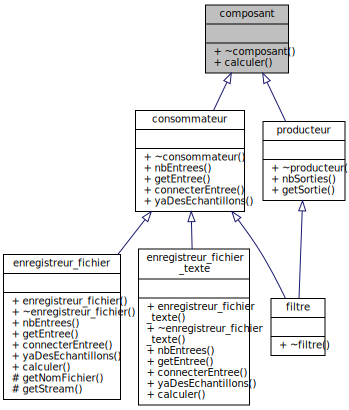
\includegraphics[width=350pt]{classcomposant__inherit__graph}
\end{center}
\end{figure}
\subsection*{Public Member Functions}
\begin{DoxyCompactItemize}
\item 
virtual \hyperlink{classcomposant_add8126876f9df35cc359f887396f0966}{$\sim$composant} ()
\begin{DoxyCompactList}\small\item\em Finaliser. \end{DoxyCompactList}\item 
virtual void \hyperlink{classcomposant_a257333d140850f51be479b025ce1e540}{calculer} ()=0
\begin{DoxyCompactList}\small\item\em Effectue les calculs associes au composant. \end{DoxyCompactList}\end{DoxyCompactItemize}


\subsection{Detailed Description}
Interface d'un composant du systeme sonore. 

\begin{DoxyAuthor}{Author}
Jean Christophe Engel, Fabrice Lamarche, University Of Rennes 1 
\end{DoxyAuthor}
\begin{DoxyDate}{Date}
23/04/2010 
\end{DoxyDate}


\subsection{Constructor \& Destructor Documentation}
\hypertarget{classcomposant_add8126876f9df35cc359f887396f0966}{\index{composant@{composant}!$\sim$composant@{$\sim$composant}}
\index{$\sim$composant@{$\sim$composant}!composant@{composant}}
\subsubsection[{$\sim$composant}]{\setlength{\rightskip}{0pt plus 5cm}composant\-::$\sim$composant (
\begin{DoxyParamCaption}
{}
\end{DoxyParamCaption}
)\hspace{0.3cm}{\ttfamily [inline]}, {\ttfamily [virtual]}}}\label{classcomposant_add8126876f9df35cc359f887396f0966}


Finaliser. 

\begin{DoxyAuthor}{Author}
Jean Christophe Engel, Fabrice Lamarche, University Of Rennes 1 
\end{DoxyAuthor}
\begin{DoxyDate}{Date}
23/04/2010 
\end{DoxyDate}


\subsection{Member Function Documentation}
\hypertarget{classcomposant_a257333d140850f51be479b025ce1e540}{\index{composant@{composant}!calculer@{calculer}}
\index{calculer@{calculer}!composant@{composant}}
\subsubsection[{calculer}]{\setlength{\rightskip}{0pt plus 5cm}void composant\-::calculer (
\begin{DoxyParamCaption}
{}
\end{DoxyParamCaption}
)\hspace{0.3cm}{\ttfamily [pure virtual]}}}\label{classcomposant_a257333d140850f51be479b025ce1e540}


Effectue les calculs associes au composant. 



Implemented in \hyperlink{classenregistreur__fichier__texte_a3c693001317b5940f3b61033c02fb2d7}{enregistreur\-\_\-fichier\-\_\-texte}, \hyperlink{classenregistreur__fichier_a3f123c156b96a9eec82bdec24962d597}{enregistreur\-\_\-fichier}, \hyperlink{classoperation__binaire_a2ecfa3c6c05006c5c1bc285281bc6f3a}{operation\-\_\-binaire$<$ T $>$}, \hyperlink{classharmonique_a4dbd729dfa443204d9834effbb63d816}{harmonique}, \hyperlink{classfiltre__compose_a6fd1598c04300da43989af4f87a37aba}{filtre\-\_\-compose}, \hyperlink{classproducteur__base_af1e171c9e69b0998d5124c7389737f82}{producteur\-\_\-base}, \hyperlink{classvolume_aab5a1f0490ea8b5826db6edd78e90f1d}{volume}, \hyperlink{classfile__reader_ac63890e9fbb85cda005efbce47f83648}{file\-\_\-reader}, \hyperlink{classsignal__constant_a18edd9db48afa7b287ae363bdcd91d43}{signal\-\_\-constant}, \hyperlink{classfiltre__base_ad06f5db1f851e5ad8655c9d8927cf347}{filtre\-\_\-base}, and \hyperlink{classmultiplicateur_ab22f15668247a10a35f027bd503f2442}{multiplicateur}.



The documentation for this class was generated from the following file\-:\begin{DoxyCompactItemize}
\item 
include/\hyperlink{composant_8h}{composant.\-h}\end{DoxyCompactItemize}

\hypertarget{classcomposant__exception}{\section{composant\-\_\-exception Class Reference}
\label{classcomposant__exception}\index{composant\-\_\-exception@{composant\-\_\-exception}}
}


classe qui gère les exceptions liées à un composant  




{\ttfamily \#include $<$composant\-\_\-exception.\-h$>$}



Inheritance diagram for composant\-\_\-exception\-:
\nopagebreak
\begin{figure}[H]
\begin{center}
\leavevmode
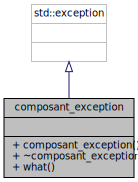
\includegraphics[width=190pt]{classcomposant__exception__inherit__graph}
\end{center}
\end{figure}


Collaboration diagram for composant\-\_\-exception\-:
\nopagebreak
\begin{figure}[H]
\begin{center}
\leavevmode
\includegraphics[width=190pt]{classcomposant__exception__coll__graph}
\end{center}
\end{figure}
\subsection*{Public Member Functions}
\begin{DoxyCompactItemize}
\item 
\hyperlink{classcomposant__exception_ae8cd86b9e3658238da8ff51a0a2c203d}{composant\-\_\-exception} (const std\-::string \&msg)
\begin{DoxyCompactList}\small\item\em initialiser une exception de composant \end{DoxyCompactList}\item 
virtual \hyperlink{classcomposant__exception_a412573cc5c9971c4be701f83a6a04b27}{$\sim$composant\-\_\-exception} ()  throw ()
\begin{DoxyCompactList}\small\item\em Destructeur. \end{DoxyCompactList}\item 
virtual const char $\ast$ \hyperlink{classcomposant__exception_aa679ff8d1a722c19de72fde0b5ad3ff5}{what} () const   throw ()
\begin{DoxyCompactList}\small\item\em Returns a C-\/style character string describing the general cause of the current error (the same string passed to the constructor). \end{DoxyCompactList}\end{DoxyCompactItemize}
\subsection*{Private Attributes}
\begin{DoxyCompactItemize}
\item 
std\-::string \hyperlink{classcomposant__exception_abe83485fc365a1e427d76b49c27b5037}{message}
\end{DoxyCompactItemize}


\subsection{Detailed Description}
classe qui gère les exceptions liées à un composant 

\begin{DoxyAuthor}{Author}
Jean Christophe Engel, Fabrice Lamarche, University Of Rennes 1 
\end{DoxyAuthor}
\begin{DoxyDate}{Date}
23/04/2010 
\end{DoxyDate}


\subsection{Constructor \& Destructor Documentation}
\hypertarget{classcomposant__exception_ae8cd86b9e3658238da8ff51a0a2c203d}{\index{composant\-\_\-exception@{composant\-\_\-exception}!composant\-\_\-exception@{composant\-\_\-exception}}
\index{composant\-\_\-exception@{composant\-\_\-exception}!composant_exception@{composant\-\_\-exception}}
\subsubsection[{composant\-\_\-exception}]{\setlength{\rightskip}{0pt plus 5cm}composant\-\_\-exception\-::composant\-\_\-exception (
\begin{DoxyParamCaption}
\item[{const std\-::string \&}]{msg}
\end{DoxyParamCaption}
)\hspace{0.3cm}{\ttfamily [inline]}}}\label{classcomposant__exception_ae8cd86b9e3658238da8ff51a0a2c203d}


initialiser une exception de composant 


\begin{DoxyParams}{Parameters}
{\em msg} & \-: texte qui décrit l'erreur \\
\hline
\end{DoxyParams}
\hypertarget{classcomposant__exception_a412573cc5c9971c4be701f83a6a04b27}{\index{composant\-\_\-exception@{composant\-\_\-exception}!$\sim$composant\-\_\-exception@{$\sim$composant\-\_\-exception}}
\index{$\sim$composant\-\_\-exception@{$\sim$composant\-\_\-exception}!composant_exception@{composant\-\_\-exception}}
\subsubsection[{$\sim$composant\-\_\-exception}]{\setlength{\rightskip}{0pt plus 5cm}composant\-\_\-exception\-::$\sim$composant\-\_\-exception (
\begin{DoxyParamCaption}
\item[{void}]{}
\end{DoxyParamCaption}
) throw  ) \hspace{0.3cm}{\ttfamily [inline]}, {\ttfamily [virtual]}}}\label{classcomposant__exception_a412573cc5c9971c4be701f83a6a04b27}


Destructeur. 



\subsection{Member Function Documentation}
\hypertarget{classcomposant__exception_aa679ff8d1a722c19de72fde0b5ad3ff5}{\index{composant\-\_\-exception@{composant\-\_\-exception}!what@{what}}
\index{what@{what}!composant_exception@{composant\-\_\-exception}}
\subsubsection[{what}]{\setlength{\rightskip}{0pt plus 5cm}const char $\ast$ composant\-\_\-exception\-::what (
\begin{DoxyParamCaption}
{}
\end{DoxyParamCaption}
) const throw  ) \hspace{0.3cm}{\ttfamily [inline]}, {\ttfamily [virtual]}}}\label{classcomposant__exception_aa679ff8d1a722c19de72fde0b5ad3ff5}


Returns a C-\/style character string describing the general cause of the current error (the same string passed to the constructor). 



\subsection{Member Data Documentation}
\hypertarget{classcomposant__exception_abe83485fc365a1e427d76b49c27b5037}{\index{composant\-\_\-exception@{composant\-\_\-exception}!message@{message}}
\index{message@{message}!composant_exception@{composant\-\_\-exception}}
\subsubsection[{message}]{\setlength{\rightskip}{0pt plus 5cm}std\-::string composant\-\_\-exception\-::message\hspace{0.3cm}{\ttfamily [private]}}}\label{classcomposant__exception_abe83485fc365a1e427d76b49c27b5037}


The documentation for this class was generated from the following file\-:\begin{DoxyCompactItemize}
\item 
include/\hyperlink{composant__exception_8h}{composant\-\_\-exception.\-h}\end{DoxyCompactItemize}

\hypertarget{classconsommateur}{\section{consommateur Class Reference}
\label{classconsommateur}\index{consommateur@{consommateur}}
}


Interface d'un consommateur d'échantillons sonores. Il s'agit d'une interface décrivant un composant qui ne possède que des entrées.  




{\ttfamily \#include $<$consommateur.\-h$>$}



Inheritance diagram for consommateur\-:
\nopagebreak
\begin{figure}[H]
\begin{center}
\leavevmode
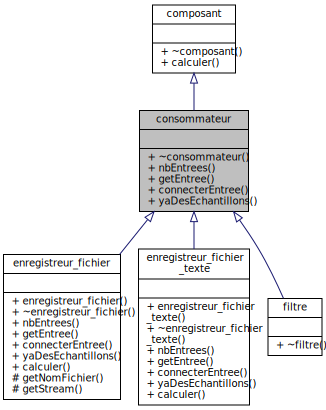
\includegraphics[width=350pt]{classconsommateur__inherit__graph}
\end{center}
\end{figure}


Collaboration diagram for consommateur\-:
\nopagebreak
\begin{figure}[H]
\begin{center}
\leavevmode
\includegraphics[width=160pt]{classconsommateur__coll__graph}
\end{center}
\end{figure}
\subsection*{Public Member Functions}
\begin{DoxyCompactItemize}
\item 
virtual \hyperlink{classconsommateur_a9a756f15381056cd7917a8022d405251}{$\sim$consommateur} ()
\begin{DoxyCompactList}\small\item\em Destructeur virtuel. \end{DoxyCompactList}\item 
virtual unsigned int \hyperlink{classconsommateur_aa06328f3002f14b5ff83e393e7e4761a}{nb\-Entrees} () const =0
\begin{DoxyCompactList}\small\item\em Renvoie le nombre d'entrees du composant. \end{DoxyCompactList}\item 
virtual const \hyperlink{classcounted__ptr}{counted\-\_\-ptr}$<$ \hyperlink{classflot}{flot} $>$ \& \hyperlink{classconsommateur_ab9d91275bf6355ffa417ceb379967af2}{get\-Entree} (unsigned int numentree) const =0
\begin{DoxyCompactList}\small\item\em Récupération d'une entrée du composant. \end{DoxyCompactList}\item 
virtual void \hyperlink{classconsommateur_a36b438c3e6c8e71989ec30441c821062}{connecter\-Entree} (const \hyperlink{classcounted__ptr}{counted\-\_\-ptr}$<$ \hyperlink{classflot}{flot} $>$ \&f, unsigned int numentree)=0
\begin{DoxyCompactList}\small\item\em Connecte une entrée sur ce composant. \end{DoxyCompactList}\item 
virtual bool \hyperlink{classconsommateur_a8622fe9e8e5baa1a7b152fce88b8be89}{ya\-Des\-Echantillons} () const =0
\begin{DoxyCompactList}\small\item\em déterminer si chaque entrée possède au moins un échantillon \end{DoxyCompactList}\end{DoxyCompactItemize}


\subsection{Detailed Description}
Interface d'un consommateur d'échantillons sonores. Il s'agit d'une interface décrivant un composant qui ne possède que des entrées. 

\begin{DoxyAuthor}{Author}
Jean Christophe Engel, Fabrice Lamarche, University Of Rennes 1 
\end{DoxyAuthor}
\begin{DoxyDate}{Date}
23/04/2010 
\end{DoxyDate}


\subsection{Constructor \& Destructor Documentation}
\hypertarget{classconsommateur_a9a756f15381056cd7917a8022d405251}{\index{consommateur@{consommateur}!$\sim$consommateur@{$\sim$consommateur}}
\index{$\sim$consommateur@{$\sim$consommateur}!consommateur@{consommateur}}
\subsubsection[{$\sim$consommateur}]{\setlength{\rightskip}{0pt plus 5cm}consommateur\-::$\sim$consommateur (
\begin{DoxyParamCaption}
{}
\end{DoxyParamCaption}
)\hspace{0.3cm}{\ttfamily [inline]}, {\ttfamily [virtual]}}}\label{classconsommateur_a9a756f15381056cd7917a8022d405251}


Destructeur virtuel. 



\subsection{Member Function Documentation}
\hypertarget{classconsommateur_a36b438c3e6c8e71989ec30441c821062}{\index{consommateur@{consommateur}!connecter\-Entree@{connecter\-Entree}}
\index{connecter\-Entree@{connecter\-Entree}!consommateur@{consommateur}}
\subsubsection[{connecter\-Entree}]{\setlength{\rightskip}{0pt plus 5cm}void consommateur\-::connecter\-Entree (
\begin{DoxyParamCaption}
\item[{const {\bf counted\-\_\-ptr}$<$ {\bf flot} $>$ \&}]{f, }
\item[{unsigned int}]{numentree}
\end{DoxyParamCaption}
)\hspace{0.3cm}{\ttfamily [pure virtual]}}}\label{classconsommateur_a36b438c3e6c8e71989ec30441c821062}


Connecte une entrée sur ce composant. 


\begin{DoxyParams}{Parameters}
{\em f} & Le flot à connecter en entrée du composant. \\
\hline
{\em numentree} & Le numéro de l'entree sur laquelle connecter le flot. \\
\hline
\end{DoxyParams}
\begin{DoxyPrecond}{Precondition}
0 $<$= numentree $<$ \hyperlink{classconsommateur_aa06328f3002f14b5ff83e393e7e4761a}{nb\-Entrees()} 
\end{DoxyPrecond}


Implemented in \hyperlink{classenregistreur__fichier__texte_a9da917c48db3891e757d971e8927dfda}{enregistreur\-\_\-fichier\-\_\-texte}, \hyperlink{classenregistreur__fichier_a3d8584ab625fab747cf8c01cc410362a}{enregistreur\-\_\-fichier}, \hyperlink{classconsommateur__base_a273d1899ba7e05e8651b4cca6aa35b1d}{consommateur\-\_\-base}, \hyperlink{classfiltre__compose_aaf4dc84a41236fb7f462d6eba569baf1}{filtre\-\_\-compose}, and \hyperlink{classvolume_a5ee6dc194dc9d47c9d554a4f94ac0512}{volume}.

\hypertarget{classconsommateur_ab9d91275bf6355ffa417ceb379967af2}{\index{consommateur@{consommateur}!get\-Entree@{get\-Entree}}
\index{get\-Entree@{get\-Entree}!consommateur@{consommateur}}
\subsubsection[{get\-Entree}]{\setlength{\rightskip}{0pt plus 5cm}const {\bf counted\-\_\-ptr}$<$ {\bf flot} $>$ \& consommateur\-::get\-Entree (
\begin{DoxyParamCaption}
\item[{unsigned int}]{numentree}
\end{DoxyParamCaption}
) const\hspace{0.3cm}{\ttfamily [pure virtual]}}}\label{classconsommateur_ab9d91275bf6355ffa417ceb379967af2}


Récupération d'une entrée du composant. 


\begin{DoxyParams}{Parameters}
{\em numentree} & Le numero de l'entrée à récuperer. \\
\hline
\end{DoxyParams}
\begin{DoxyPrecond}{Precondition}
0 $<$= numentree $<$ \hyperlink{classconsommateur_aa06328f3002f14b5ff83e393e7e4761a}{nb\-Entrees()} 
\end{DoxyPrecond}
\begin{DoxyReturn}{Returns}
L'entrée demandée. 
\end{DoxyReturn}


Implemented in \hyperlink{classenregistreur__fichier__texte_a065dcf79e74d6d7388dbb2909c0d2be2}{enregistreur\-\_\-fichier\-\_\-texte}, \hyperlink{classenregistreur__fichier_a45c98f8a93f4f6b5ac733248769aebb5}{enregistreur\-\_\-fichier}, and \hyperlink{classconsommateur__base_aaa04503aa9b028729a0dbaf0d5a6d63c}{consommateur\-\_\-base}.

\hypertarget{classconsommateur_aa06328f3002f14b5ff83e393e7e4761a}{\index{consommateur@{consommateur}!nb\-Entrees@{nb\-Entrees}}
\index{nb\-Entrees@{nb\-Entrees}!consommateur@{consommateur}}
\subsubsection[{nb\-Entrees}]{\setlength{\rightskip}{0pt plus 5cm}unsigned int consommateur\-::nb\-Entrees (
\begin{DoxyParamCaption}
{}
\end{DoxyParamCaption}
) const\hspace{0.3cm}{\ttfamily [pure virtual]}}}\label{classconsommateur_aa06328f3002f14b5ff83e393e7e4761a}


Renvoie le nombre d'entrees du composant. 

\begin{DoxyReturn}{Returns}
Le nombre d'entrees du composant. 
\end{DoxyReturn}


Implemented in \hyperlink{classenregistreur__fichier__texte_a0f686274b3cca79fba1d3c2227cd4950}{enregistreur\-\_\-fichier\-\_\-texte}, \hyperlink{classenregistreur__fichier_a46b864aea1016ecef695e085870706af}{enregistreur\-\_\-fichier}, and \hyperlink{classconsommateur__base_a71244a18e367c260320ab220c416d83a}{consommateur\-\_\-base}.

\hypertarget{classconsommateur_a8622fe9e8e5baa1a7b152fce88b8be89}{\index{consommateur@{consommateur}!ya\-Des\-Echantillons@{ya\-Des\-Echantillons}}
\index{ya\-Des\-Echantillons@{ya\-Des\-Echantillons}!consommateur@{consommateur}}
\subsubsection[{ya\-Des\-Echantillons}]{\setlength{\rightskip}{0pt plus 5cm}bool consommateur\-::ya\-Des\-Echantillons (
\begin{DoxyParamCaption}
{}
\end{DoxyParamCaption}
) const\hspace{0.3cm}{\ttfamily [pure virtual]}}}\label{classconsommateur_a8622fe9e8e5baa1a7b152fce88b8be89}


déterminer si chaque entrée possède au moins un échantillon 

\begin{DoxyReturn}{Returns}
Vrai si chaque entrée possède au moins un échantillon. 
\end{DoxyReturn}


Implemented in \hyperlink{classenregistreur__fichier__texte_ac412238ca34c019727aa6ddfbe9ae56e}{enregistreur\-\_\-fichier\-\_\-texte}, \hyperlink{classenregistreur__fichier_a1f20e9ef18665e9b3714d067b573a9de}{enregistreur\-\_\-fichier}, and \hyperlink{classconsommateur__base_a19f135d483c30324526d63c18a536f36}{consommateur\-\_\-base}.



The documentation for this class was generated from the following file\-:\begin{DoxyCompactItemize}
\item 
include/\hyperlink{consommateur_8h}{consommateur.\-h}\end{DoxyCompactItemize}

\hypertarget{classconsommateur__base}{\section{consommateur\-\_\-base Class Reference}
\label{classconsommateur__base}\index{consommateur\-\_\-base@{consommateur\-\_\-base}}
}


{\ttfamily \#include $<$consommateur\-\_\-base.\-h$>$}



Inheritance diagram for consommateur\-\_\-base\-:
\nopagebreak
\begin{figure}[H]
\begin{center}
\leavevmode
\includegraphics[width=350pt]{classconsommateur__base__inherit__graph}
\end{center}
\end{figure}


Collaboration diagram for consommateur\-\_\-base\-:
\nopagebreak
\begin{figure}[H]
\begin{center}
\leavevmode
\includegraphics[width=186pt]{classconsommateur__base__coll__graph}
\end{center}
\end{figure}
\subsection*{Public Member Functions}
\begin{DoxyCompactItemize}
\item 
\hyperlink{classconsommateur__base_a3a96b41f2a05573c8be4a820462f73dc}{consommateur\-\_\-base} (unsigned int)
\item 
virtual \hyperlink{classconsommateur__base_a8c5da6cd2134ad9cc76a8d8ddf303b91}{$\sim$consommateur\-\_\-base} ()
\item 
virtual unsigned int \hyperlink{classconsommateur__base_a71244a18e367c260320ab220c416d83a}{nb\-Entrees} () const 
\item 
virtual const \hyperlink{classcounted__ptr}{counted\-\_\-ptr}$<$ \hyperlink{classflot}{flot} $>$ \& \hyperlink{classconsommateur__base_aaa04503aa9b028729a0dbaf0d5a6d63c}{get\-Entree} (unsigned int) const 
\item 
virtual void \hyperlink{classconsommateur__base_a273d1899ba7e05e8651b4cca6aa35b1d}{connecter\-Entree} (const \hyperlink{classcounted__ptr}{counted\-\_\-ptr}$<$ \hyperlink{classflot}{flot} $>$ \&, unsigned int)
\item 
virtual bool \hyperlink{classconsommateur__base_a19f135d483c30324526d63c18a536f36}{ya\-Des\-Echantillons} () const 
\end{DoxyCompactItemize}
\subsection*{Protected Attributes}
\begin{DoxyCompactItemize}
\item 
unsigned int \hyperlink{classconsommateur__base_af75625bb7dc752ff9aa173c6aff50059}{m\-\_\-max\-\_\-input}
\item 
std\-::vector$<$ \hyperlink{classcounted__ptr}{counted\-\_\-ptr}$<$ \hyperlink{classflot}{flot} $>$ $>$ \hyperlink{classconsommateur__base_a061094bb0041f748ff88d94b1e503087}{m\-\_\-input}
\end{DoxyCompactItemize}


\subsection{Constructor \& Destructor Documentation}
\hypertarget{classconsommateur__base_a3a96b41f2a05573c8be4a820462f73dc}{\index{consommateur\-\_\-base@{consommateur\-\_\-base}!consommateur\-\_\-base@{consommateur\-\_\-base}}
\index{consommateur\-\_\-base@{consommateur\-\_\-base}!consommateur_base@{consommateur\-\_\-base}}
\subsubsection[{consommateur\-\_\-base}]{\setlength{\rightskip}{0pt plus 5cm}consommateur\-\_\-base\-::consommateur\-\_\-base (
\begin{DoxyParamCaption}
\item[{unsigned int}]{nb\-Out}
\end{DoxyParamCaption}
)}}\label{classconsommateur__base_a3a96b41f2a05573c8be4a820462f73dc}
Construit un consommateur avec nb\-Out sorties \hypertarget{classconsommateur__base_a8c5da6cd2134ad9cc76a8d8ddf303b91}{\index{consommateur\-\_\-base@{consommateur\-\_\-base}!$\sim$consommateur\-\_\-base@{$\sim$consommateur\-\_\-base}}
\index{$\sim$consommateur\-\_\-base@{$\sim$consommateur\-\_\-base}!consommateur_base@{consommateur\-\_\-base}}
\subsubsection[{$\sim$consommateur\-\_\-base}]{\setlength{\rightskip}{0pt plus 5cm}virtual consommateur\-\_\-base\-::$\sim$consommateur\-\_\-base (
\begin{DoxyParamCaption}
{}
\end{DoxyParamCaption}
)\hspace{0.3cm}{\ttfamily [inline]}, {\ttfamily [virtual]}}}\label{classconsommateur__base_a8c5da6cd2134ad9cc76a8d8ddf303b91}


\subsection{Member Function Documentation}
\hypertarget{classconsommateur__base_a273d1899ba7e05e8651b4cca6aa35b1d}{\index{consommateur\-\_\-base@{consommateur\-\_\-base}!connecter\-Entree@{connecter\-Entree}}
\index{connecter\-Entree@{connecter\-Entree}!consommateur_base@{consommateur\-\_\-base}}
\subsubsection[{connecter\-Entree}]{\setlength{\rightskip}{0pt plus 5cm}void consommateur\-\_\-base\-::connecter\-Entree (
\begin{DoxyParamCaption}
\item[{const {\bf counted\-\_\-ptr}$<$ {\bf flot} $>$ \&}]{fl, }
\item[{unsigned int}]{nb\-In}
\end{DoxyParamCaption}
)\hspace{0.3cm}{\ttfamily [virtual]}}}\label{classconsommateur__base_a273d1899ba7e05e8651b4cca6aa35b1d}
Connecte un flot fl à l'entrée nb\-In 

Implements \hyperlink{classconsommateur_a36b438c3e6c8e71989ec30441c821062}{consommateur}.



Reimplemented in \hyperlink{classfiltre__compose_aaf4dc84a41236fb7f462d6eba569baf1}{filtre\-\_\-compose}, and \hyperlink{classvolume_a5ee6dc194dc9d47c9d554a4f94ac0512}{volume}.

\hypertarget{classconsommateur__base_aaa04503aa9b028729a0dbaf0d5a6d63c}{\index{consommateur\-\_\-base@{consommateur\-\_\-base}!get\-Entree@{get\-Entree}}
\index{get\-Entree@{get\-Entree}!consommateur_base@{consommateur\-\_\-base}}
\subsubsection[{get\-Entree}]{\setlength{\rightskip}{0pt plus 5cm}const {\bf counted\-\_\-ptr}$<$ {\bf flot} $>$ \& consommateur\-\_\-base\-::get\-Entree (
\begin{DoxyParamCaption}
\item[{unsigned int}]{nb\-Out}
\end{DoxyParamCaption}
) const\hspace{0.3cm}{\ttfamily [virtual]}}}\label{classconsommateur__base_aaa04503aa9b028729a0dbaf0d5a6d63c}
Récupère le flot à l'entrée nb\-Out 

Implements \hyperlink{classconsommateur_ab9d91275bf6355ffa417ceb379967af2}{consommateur}.

\hypertarget{classconsommateur__base_a71244a18e367c260320ab220c416d83a}{\index{consommateur\-\_\-base@{consommateur\-\_\-base}!nb\-Entrees@{nb\-Entrees}}
\index{nb\-Entrees@{nb\-Entrees}!consommateur_base@{consommateur\-\_\-base}}
\subsubsection[{nb\-Entrees}]{\setlength{\rightskip}{0pt plus 5cm}unsigned int consommateur\-\_\-base\-::nb\-Entrees (
\begin{DoxyParamCaption}
{}
\end{DoxyParamCaption}
) const\hspace{0.3cm}{\ttfamily [virtual]}}}\label{classconsommateur__base_a71244a18e367c260320ab220c416d83a}
Renvoie le nombre d'entrées de ce consommateur 

Implements \hyperlink{classconsommateur_aa06328f3002f14b5ff83e393e7e4761a}{consommateur}.

\hypertarget{classconsommateur__base_a19f135d483c30324526d63c18a536f36}{\index{consommateur\-\_\-base@{consommateur\-\_\-base}!ya\-Des\-Echantillons@{ya\-Des\-Echantillons}}
\index{ya\-Des\-Echantillons@{ya\-Des\-Echantillons}!consommateur_base@{consommateur\-\_\-base}}
\subsubsection[{ya\-Des\-Echantillons}]{\setlength{\rightskip}{0pt plus 5cm}bool consommateur\-\_\-base\-::ya\-Des\-Echantillons (
\begin{DoxyParamCaption}
{}
\end{DoxyParamCaption}
) const\hspace{0.3cm}{\ttfamily [virtual]}}}\label{classconsommateur__base_a19f135d483c30324526d63c18a536f36}
Le flot possède-\/t-\/il des échantillons 

Implements \hyperlink{classconsommateur_a8622fe9e8e5baa1a7b152fce88b8be89}{consommateur}.



\subsection{Member Data Documentation}
\hypertarget{classconsommateur__base_a061094bb0041f748ff88d94b1e503087}{\index{consommateur\-\_\-base@{consommateur\-\_\-base}!m\-\_\-input@{m\-\_\-input}}
\index{m\-\_\-input@{m\-\_\-input}!consommateur_base@{consommateur\-\_\-base}}
\subsubsection[{m\-\_\-input}]{\setlength{\rightskip}{0pt plus 5cm}std\-::vector$<${\bf counted\-\_\-ptr}$<${\bf flot}$>$ $>$ consommateur\-\_\-base\-::m\-\_\-input\hspace{0.3cm}{\ttfamily [protected]}}}\label{classconsommateur__base_a061094bb0041f748ff88d94b1e503087}
Liste des entrées \hypertarget{classconsommateur__base_af75625bb7dc752ff9aa173c6aff50059}{\index{consommateur\-\_\-base@{consommateur\-\_\-base}!m\-\_\-max\-\_\-input@{m\-\_\-max\-\_\-input}}
\index{m\-\_\-max\-\_\-input@{m\-\_\-max\-\_\-input}!consommateur_base@{consommateur\-\_\-base}}
\subsubsection[{m\-\_\-max\-\_\-input}]{\setlength{\rightskip}{0pt plus 5cm}unsigned int consommateur\-\_\-base\-::m\-\_\-max\-\_\-input\hspace{0.3cm}{\ttfamily [protected]}}}\label{classconsommateur__base_af75625bb7dc752ff9aa173c6aff50059}
Nombre d'entrées sur ce consommateur 

The documentation for this class was generated from the following files\-:\begin{DoxyCompactItemize}
\item 
src/\hyperlink{consommateur__base_8h}{consommateur\-\_\-base.\-h}\item 
src/\hyperlink{consommateur__base_8cpp}{consommateur\-\_\-base.\-cpp}\end{DoxyCompactItemize}

\hypertarget{classcounted__ptr}{\section{counted\-\_\-ptr$<$ T $>$ Class Template Reference}
\label{classcounted__ptr}\index{counted\-\_\-ptr$<$ T $>$@{counted\-\_\-ptr$<$ T $>$}}
}


Classe gérant un \char`\"{}smart pointer\char`\"{}.  




{\ttfamily \#include $<$counted\-\_\-ptr.\-h$>$}

\subsection*{Public Member Functions}
\begin{DoxyCompactItemize}
\item 
\hyperlink{classcounted__ptr_afc15d9bc04c1be60099294037e9cbdc1}{counted\-\_\-ptr} (T $\ast$pointer=0)
\begin{DoxyCompactList}\small\item\em Constructeur. \end{DoxyCompactList}\item 
virtual \hyperlink{classcounted__ptr_a8b23efee2c3349c85b0acb9cb0c02b88}{$\sim$counted\-\_\-ptr} ()
\begin{DoxyCompactList}\small\item\em Destructeur, libère la donnée s'il s'agit du dernier pointeur qui la désigne. \end{DoxyCompactList}\item 
\hyperlink{classcounted__ptr_a761e66ebb626a54888dd3f29093d02f2}{counted\-\_\-ptr} (const \hyperlink{classcounted__ptr}{counted\-\_\-ptr} \&smart\-Pointer)
\begin{DoxyCompactList}\small\item\em Constructeur de copie. \end{DoxyCompactList}\item 
\hyperlink{classcounted__ptr}{counted\-\_\-ptr} \& \hyperlink{classcounted__ptr_a66a449e044736694d639c0077d1e1053}{operator=} (const \hyperlink{classcounted__ptr}{counted\-\_\-ptr} \&smart\-Pointer)
\begin{DoxyCompactList}\small\item\em Opérateur d'affectation. \end{DoxyCompactList}\item 
{\footnotesize template$<$class U $>$ }\\\hyperlink{classcounted__ptr_afcd57d6c61d5774e1397da21a0e2f875}{counted\-\_\-ptr} (const \hyperlink{classcounted__ptr}{counted\-\_\-ptr}$<$ U $>$ \&smart\-Pointer)
\begin{DoxyCompactList}\small\item\em Constructeur de transtypage. Permet de pointer sur une instance de classe U via un pointeur de type T, U héritant T. \end{DoxyCompactList}\item 
bool \hyperlink{classcounted__ptr_a4d951309592e9186940afe98c07ed72e}{isnull} () const 
\item 
T \& \hyperlink{classcounted__ptr_aa7b22a5b53011b29dbebab1ec7acbe17}{operator$\ast$} () const 
\begin{DoxyCompactList}\small\item\em Accès à la variable désignée par le pointeur. \end{DoxyCompactList}\item 
T $\ast$ \hyperlink{classcounted__ptr_aa50f9c6eee8e60d42a8fa6fff232be6c}{operator-\/$>$} () const 
\begin{DoxyCompactList}\small\item\em Opérateur d'accès aux attributs / méthodes de la variable pointée. \end{DoxyCompactList}\end{DoxyCompactItemize}
\subsection*{Private Member Functions}
\begin{DoxyCompactItemize}
\item 
void \hyperlink{classcounted__ptr_a1e2f4d7eb63dd5757e9a3f2f701423a3}{acquerir} (const \hyperlink{classcounted__ptr}{counted\-\_\-ptr}$<$ T $>$ \&cp)
\item 
{\footnotesize template$<$class U $>$ }\\void \hyperlink{classcounted__ptr_a895493d30acc074bcdb2debd4978427a}{acquerir} (const \hyperlink{classcounted__ptr}{counted\-\_\-ptr}$<$ U $>$ \&cp)
\item 
void \hyperlink{classcounted__ptr_a0b9693015481176159f87f26e530409d}{liberer} ()
\end{DoxyCompactItemize}
\subsection*{Private Attributes}
\begin{DoxyCompactItemize}
\item 
unsigned int $\ast$ \hyperlink{classcounted__ptr_abf02f680f71697211394ebdfb47f14ff}{m\-\_\-counter}
\item 
T $\ast$ \hyperlink{classcounted__ptr_adfc589214b83bdd53c7640d8374f1098}{m\-\_\-ptr}
\end{DoxyCompactItemize}
\subsection*{Friends}
\begin{DoxyCompactItemize}
\item 
{\footnotesize template$<$class U $>$ }\\class \hyperlink{classcounted__ptr_abf29d1b6b221e60964e0852b2518841a}{counted\-\_\-ptr}
\begin{DoxyCompactList}\small\item\em Donner à counted\-\_\-ptr$<$\-U$>$ accès à la partie privée de counted\-\_\-ptr$<$\-T$>$ \end{DoxyCompactList}\end{DoxyCompactItemize}


\subsection{Detailed Description}
\subsubsection*{template$<$class T$>$class counted\-\_\-ptr$<$ T $>$}

Classe gérant un \char`\"{}smart pointer\char`\"{}. 

\begin{DoxyAuthor}{Author}
Jean Christophe Engel, Fabrice Lamarche, University Of Rennes 1 
\end{DoxyAuthor}
\begin{DoxyDate}{Date}
23/04/2010 
\end{DoxyDate}


\subsection{Constructor \& Destructor Documentation}
\hypertarget{classcounted__ptr_afc15d9bc04c1be60099294037e9cbdc1}{\index{counted\-\_\-ptr@{counted\-\_\-ptr}!counted\-\_\-ptr@{counted\-\_\-ptr}}
\index{counted\-\_\-ptr@{counted\-\_\-ptr}!counted_ptr@{counted\-\_\-ptr}}
\subsubsection[{counted\-\_\-ptr}]{\setlength{\rightskip}{0pt plus 5cm}template$<$class T $>$ {\bf counted\-\_\-ptr}$<$ T $>$\-::{\bf counted\-\_\-ptr} (
\begin{DoxyParamCaption}
\item[{T $\ast$}]{pointer = {\ttfamily 0}}
\end{DoxyParamCaption}
)\hspace{0.3cm}{\ttfamily [explicit]}}}\label{classcounted__ptr_afc15d9bc04c1be60099294037e9cbdc1}


Constructeur. 


\begin{DoxyParams}{Parameters}
{\em pointer} & Si non nul, un pointeur vers une variable allouée dynamiquement.\\
\hline
\end{DoxyParams}


 \subsubsection*{méthodes publiques }\hypertarget{classcounted__ptr_a8b23efee2c3349c85b0acb9cb0c02b88}{\index{counted\-\_\-ptr@{counted\-\_\-ptr}!$\sim$counted\-\_\-ptr@{$\sim$counted\-\_\-ptr}}
\index{$\sim$counted\-\_\-ptr@{$\sim$counted\-\_\-ptr}!counted_ptr@{counted\-\_\-ptr}}
\subsubsection[{$\sim$counted\-\_\-ptr}]{\setlength{\rightskip}{0pt plus 5cm}template$<$class T $>$ {\bf counted\-\_\-ptr}$<$ T $>$\-::$\sim${\bf counted\-\_\-ptr} (
\begin{DoxyParamCaption}
\item[{void}]{}
\end{DoxyParamCaption}
)\hspace{0.3cm}{\ttfamily [virtual]}}}\label{classcounted__ptr_a8b23efee2c3349c85b0acb9cb0c02b88}


Destructeur, libère la donnée s'il s'agit du dernier pointeur qui la désigne. 

\hypertarget{classcounted__ptr_a761e66ebb626a54888dd3f29093d02f2}{\index{counted\-\_\-ptr@{counted\-\_\-ptr}!counted\-\_\-ptr@{counted\-\_\-ptr}}
\index{counted\-\_\-ptr@{counted\-\_\-ptr}!counted_ptr@{counted\-\_\-ptr}}
\subsubsection[{counted\-\_\-ptr}]{\setlength{\rightskip}{0pt plus 5cm}template$<$class T $>$ {\bf counted\-\_\-ptr}$<$ T $>$\-::{\bf counted\-\_\-ptr} (
\begin{DoxyParamCaption}
\item[{const {\bf counted\-\_\-ptr}$<$ T $>$ \&}]{smart\-Pointer}
\end{DoxyParamCaption}
)}}\label{classcounted__ptr_a761e66ebb626a54888dd3f29093d02f2}


Constructeur de copie. 


\begin{DoxyParams}{Parameters}
{\em smart\-Pointer} & \-: le \char`\"{}smart pointer\char`\"{} à copier. \\
\hline
\end{DoxyParams}
\hypertarget{classcounted__ptr_afcd57d6c61d5774e1397da21a0e2f875}{\index{counted\-\_\-ptr@{counted\-\_\-ptr}!counted\-\_\-ptr@{counted\-\_\-ptr}}
\index{counted\-\_\-ptr@{counted\-\_\-ptr}!counted_ptr@{counted\-\_\-ptr}}
\subsubsection[{counted\-\_\-ptr}]{\setlength{\rightskip}{0pt plus 5cm}template$<$class T $>$ template$<$class U $>$ {\bf counted\-\_\-ptr}$<$ T $>$\-::{\bf counted\-\_\-ptr} (
\begin{DoxyParamCaption}
\item[{const {\bf counted\-\_\-ptr}$<$ U $>$ \&}]{smart\-Pointer}
\end{DoxyParamCaption}
)}}\label{classcounted__ptr_afcd57d6c61d5774e1397da21a0e2f875}


Constructeur de transtypage. Permet de pointer sur une instance de classe U via un pointeur de type T, U héritant T. 


\begin{DoxyParams}{Parameters}
{\em smart\-Pointer} & \\
\hline
\end{DoxyParams}


\subsection{Member Function Documentation}
\hypertarget{classcounted__ptr_a1e2f4d7eb63dd5757e9a3f2f701423a3}{\index{counted\-\_\-ptr@{counted\-\_\-ptr}!acquerir@{acquerir}}
\index{acquerir@{acquerir}!counted_ptr@{counted\-\_\-ptr}}
\subsubsection[{acquerir}]{\setlength{\rightskip}{0pt plus 5cm}template$<$class T $>$ void {\bf counted\-\_\-ptr}$<$ T $>$\-::acquerir (
\begin{DoxyParamCaption}
\item[{const {\bf counted\-\_\-ptr}$<$ T $>$ \&}]{cp}
\end{DoxyParamCaption}
)\hspace{0.3cm}{\ttfamily [private]}}}\label{classcounted__ptr_a1e2f4d7eb63dd5757e9a3f2f701423a3}
\hypertarget{classcounted__ptr_a895493d30acc074bcdb2debd4978427a}{\index{counted\-\_\-ptr@{counted\-\_\-ptr}!acquerir@{acquerir}}
\index{acquerir@{acquerir}!counted_ptr@{counted\-\_\-ptr}}
\subsubsection[{acquerir}]{\setlength{\rightskip}{0pt plus 5cm}template$<$class T $>$ template$<$class U $>$ void {\bf counted\-\_\-ptr}$<$ T $>$\-::acquerir (
\begin{DoxyParamCaption}
\item[{const {\bf counted\-\_\-ptr}$<$ U $>$ \&}]{cp}
\end{DoxyParamCaption}
)\hspace{0.3cm}{\ttfamily [private]}}}\label{classcounted__ptr_a895493d30acc074bcdb2debd4978427a}
\hypertarget{classcounted__ptr_a4d951309592e9186940afe98c07ed72e}{\index{counted\-\_\-ptr@{counted\-\_\-ptr}!isnull@{isnull}}
\index{isnull@{isnull}!counted_ptr@{counted\-\_\-ptr}}
\subsubsection[{isnull}]{\setlength{\rightskip}{0pt plus 5cm}template$<$class T $>$ bool {\bf counted\-\_\-ptr}$<$ T $>$\-::isnull (
\begin{DoxyParamCaption}
{}
\end{DoxyParamCaption}
) const}}\label{classcounted__ptr_a4d951309592e9186940afe98c07ed72e}
\begin{DoxyReturn}{Returns}
vrai si le pointeur ne désigne rien 
\end{DoxyReturn}
\hypertarget{classcounted__ptr_a0b9693015481176159f87f26e530409d}{\index{counted\-\_\-ptr@{counted\-\_\-ptr}!liberer@{liberer}}
\index{liberer@{liberer}!counted_ptr@{counted\-\_\-ptr}}
\subsubsection[{liberer}]{\setlength{\rightskip}{0pt plus 5cm}template$<$class T $>$ void {\bf counted\-\_\-ptr}$<$ T $>$\-::liberer (
\begin{DoxyParamCaption}
{}
\end{DoxyParamCaption}
)\hspace{0.3cm}{\ttfamily [private]}}}\label{classcounted__ptr_a0b9693015481176159f87f26e530409d}
\hypertarget{classcounted__ptr_aa7b22a5b53011b29dbebab1ec7acbe17}{\index{counted\-\_\-ptr@{counted\-\_\-ptr}!operator$\ast$@{operator$\ast$}}
\index{operator$\ast$@{operator$\ast$}!counted_ptr@{counted\-\_\-ptr}}
\subsubsection[{operator$\ast$}]{\setlength{\rightskip}{0pt plus 5cm}template$<$class T $>$ T \& {\bf counted\-\_\-ptr}$<$ T $>$\-::operator$\ast$ (
\begin{DoxyParamCaption}
{}
\end{DoxyParamCaption}
) const}}\label{classcounted__ptr_aa7b22a5b53011b29dbebab1ec7acbe17}


Accès à la variable désignée par le pointeur. 

\begin{DoxyReturn}{Returns}
La variable désignée par le pointeur. 
\end{DoxyReturn}
\hypertarget{classcounted__ptr_aa50f9c6eee8e60d42a8fa6fff232be6c}{\index{counted\-\_\-ptr@{counted\-\_\-ptr}!operator-\/$>$@{operator-\/$>$}}
\index{operator-\/$>$@{operator-\/$>$}!counted_ptr@{counted\-\_\-ptr}}
\subsubsection[{operator-\/$>$}]{\setlength{\rightskip}{0pt plus 5cm}template$<$class T $>$ T $\ast$ {\bf counted\-\_\-ptr}$<$ T $>$\-::operator-\/$>$ (
\begin{DoxyParamCaption}
{}
\end{DoxyParamCaption}
) const}}\label{classcounted__ptr_aa50f9c6eee8e60d42a8fa6fff232be6c}


Opérateur d'accès aux attributs / méthodes de la variable pointée. 

\begin{DoxyReturn}{Returns}
adresse de la variable désignée par le pointeur. 
\end{DoxyReturn}
\hypertarget{classcounted__ptr_a66a449e044736694d639c0077d1e1053}{\index{counted\-\_\-ptr@{counted\-\_\-ptr}!operator=@{operator=}}
\index{operator=@{operator=}!counted_ptr@{counted\-\_\-ptr}}
\subsubsection[{operator=}]{\setlength{\rightskip}{0pt plus 5cm}template$<$class T $>$ {\bf counted\-\_\-ptr}$<$ T $>$ \& {\bf counted\-\_\-ptr}$<$ T $>$\-::operator= (
\begin{DoxyParamCaption}
\item[{const {\bf counted\-\_\-ptr}$<$ T $>$ \&}]{smart\-Pointer}
\end{DoxyParamCaption}
)}}\label{classcounted__ptr_a66a449e044736694d639c0077d1e1053}


Opérateur d'affectation. 


\begin{DoxyParams}{Parameters}
{\em smart\-Pointer} & \-: l'opérande de droite de l'affectation. \\
\hline
\end{DoxyParams}


\subsection{Friends And Related Function Documentation}
\hypertarget{classcounted__ptr_abf29d1b6b221e60964e0852b2518841a}{\index{counted\-\_\-ptr@{counted\-\_\-ptr}!counted\-\_\-ptr@{counted\-\_\-ptr}}
\index{counted\-\_\-ptr@{counted\-\_\-ptr}!counted_ptr@{counted\-\_\-ptr}}
\subsubsection[{counted\-\_\-ptr}]{\setlength{\rightskip}{0pt plus 5cm}template$<$class T$>$ template$<$class U $>$ friend class {\bf counted\-\_\-ptr}\hspace{0.3cm}{\ttfamily [friend]}}}\label{classcounted__ptr_abf29d1b6b221e60964e0852b2518841a}


Donner à counted\-\_\-ptr$<$\-U$>$ accès à la partie privée de counted\-\_\-ptr$<$\-T$>$ 



\subsection{Member Data Documentation}
\hypertarget{classcounted__ptr_abf02f680f71697211394ebdfb47f14ff}{\index{counted\-\_\-ptr@{counted\-\_\-ptr}!m\-\_\-counter@{m\-\_\-counter}}
\index{m\-\_\-counter@{m\-\_\-counter}!counted_ptr@{counted\-\_\-ptr}}
\subsubsection[{m\-\_\-counter}]{\setlength{\rightskip}{0pt plus 5cm}template$<$class T$>$ unsigned int$\ast$ {\bf counted\-\_\-ptr}$<$ T $>$\-::m\-\_\-counter\hspace{0.3cm}{\ttfamily [private]}}}\label{classcounted__ptr_abf02f680f71697211394ebdfb47f14ff}
\hypertarget{classcounted__ptr_adfc589214b83bdd53c7640d8374f1098}{\index{counted\-\_\-ptr@{counted\-\_\-ptr}!m\-\_\-ptr@{m\-\_\-ptr}}
\index{m\-\_\-ptr@{m\-\_\-ptr}!counted_ptr@{counted\-\_\-ptr}}
\subsubsection[{m\-\_\-ptr}]{\setlength{\rightskip}{0pt plus 5cm}template$<$class T$>$ T$\ast$ {\bf counted\-\_\-ptr}$<$ T $>$\-::m\-\_\-ptr\hspace{0.3cm}{\ttfamily [private]}}}\label{classcounted__ptr_adfc589214b83bdd53c7640d8374f1098}


The documentation for this class was generated from the following file\-:\begin{DoxyCompactItemize}
\item 
include/\hyperlink{counted__ptr_8h}{counted\-\_\-ptr.\-h}\end{DoxyCompactItemize}

\hypertarget{classenregistreur__fichier}{\section{enregistreur\-\_\-fichier Class Reference}
\label{classenregistreur__fichier}\index{enregistreur\-\_\-fichier@{enregistreur\-\_\-fichier}}
}


Un consommateur qui enregistre ses entrées dans un fichier binaire ; 44100 Hz, 16bits signé, entrelacé  




{\ttfamily \#include $<$enregistreur\-\_\-fichier.\-h$>$}



Inheritance diagram for enregistreur\-\_\-fichier\-:
\nopagebreak
\begin{figure}[H]
\begin{center}
\leavevmode
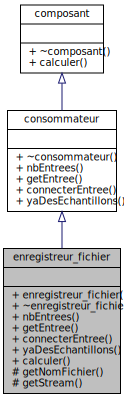
\includegraphics[width=178pt]{classenregistreur__fichier__inherit__graph}
\end{center}
\end{figure}


Collaboration diagram for enregistreur\-\_\-fichier\-:
\nopagebreak
\begin{figure}[H]
\begin{center}
\leavevmode
\includegraphics[width=178pt]{classenregistreur__fichier__coll__graph}
\end{center}
\end{figure}
\subsection*{Public Member Functions}
\begin{DoxyCompactItemize}
\item 
\hyperlink{classenregistreur__fichier_ab8eb72e794d29c47dc3476259de2836c}{enregistreur\-\_\-fichier} (std\-::string nf, unsigned int nbc)
\begin{DoxyCompactList}\small\item\em initialise le flux de sortie \end{DoxyCompactList}\item 
virtual \hyperlink{classenregistreur__fichier_a34d78a6c1510f953ca2d66a2767e2dfd}{$\sim$enregistreur\-\_\-fichier} ()
\begin{DoxyCompactList}\small\item\em Destructeur virtuel. ; ferme le fichier. \end{DoxyCompactList}\item 
unsigned int \hyperlink{classenregistreur__fichier_a46b864aea1016ecef695e085870706af}{nb\-Entrees} () const 
\item 
virtual const \hyperlink{classcounted__ptr}{counted\-\_\-ptr}$<$ \hyperlink{classflot}{flot} $>$ \& \hyperlink{classenregistreur__fichier_a45c98f8a93f4f6b5ac733248769aebb5}{get\-Entree} (unsigned int numentree) const 
\item 
virtual void \hyperlink{classenregistreur__fichier_a3d8584ab625fab747cf8c01cc410362a}{connecter\-Entree} (const \hyperlink{classcounted__ptr}{counted\-\_\-ptr}$<$ \hyperlink{classflot}{flot} $>$ \&f, unsigned int numentree)
\begin{DoxyCompactList}\small\item\em Connecte une entrée sur ce composant. \end{DoxyCompactList}\item 
virtual bool \hyperlink{classenregistreur__fichier_a1f20e9ef18665e9b3714d067b573a9de}{ya\-Des\-Echantillons} () const 
\item 
virtual void \hyperlink{classenregistreur__fichier_a3f123c156b96a9eec82bdec24962d597}{calculer} ()
\begin{DoxyCompactList}\small\item\em Effectue les calculs associes au composant. \end{DoxyCompactList}\end{DoxyCompactItemize}
\subsection*{Protected Member Functions}
\begin{DoxyCompactItemize}
\item 
const std\-::string \& \hyperlink{classenregistreur__fichier_a86ad2c3ffecb4f12f057e0d63e7bbb7f}{get\-Nom\-Fichier} () const 
\item 
std\-::ofstream \& \hyperlink{classenregistreur__fichier_a7781a7305c09f3777cbf96a0d06ddfb4}{get\-Stream} ()
\end{DoxyCompactItemize}
\subsection*{Private Attributes}
\begin{DoxyCompactItemize}
\item 
int \hyperlink{classenregistreur__fichier_a18b256b717938088893ac6c836079428}{m\-\_\-nb\-E}
\item 
std\-::vector$<$ \hyperlink{classcounted__ptr}{counted\-\_\-ptr}$<$ \hyperlink{classflot}{flot} $>$ $>$ \hyperlink{classenregistreur__fichier_a27e5d8ef895fc1bacf7dd20fe7532373}{m\-\_\-les\-Entrees}
\item 
std\-::string \hyperlink{classenregistreur__fichier_a2112179ea9e7bba0eb1cdbd8e627d695}{m\-\_\-nom\-Fichier}
\item 
std\-::ofstream \hyperlink{classenregistreur__fichier_a878b033faa126b12ad6080fe1a159c70}{m\-\_\-flux\-Sortie}
\end{DoxyCompactItemize}


\subsection{Detailed Description}
Un consommateur qui enregistre ses entrées dans un fichier binaire ; 44100 Hz, 16bits signé, entrelacé 

\begin{DoxyAuthor}{Author}
Jean Christophe Engel, Fabrice Lamarche, University Of Rennes 1 
\end{DoxyAuthor}
\begin{DoxyDate}{Date}
23/04/2010 
\end{DoxyDate}


\subsection{Constructor \& Destructor Documentation}
\hypertarget{classenregistreur__fichier_ab8eb72e794d29c47dc3476259de2836c}{\index{enregistreur\-\_\-fichier@{enregistreur\-\_\-fichier}!enregistreur\-\_\-fichier@{enregistreur\-\_\-fichier}}
\index{enregistreur\-\_\-fichier@{enregistreur\-\_\-fichier}!enregistreur_fichier@{enregistreur\-\_\-fichier}}
\subsubsection[{enregistreur\-\_\-fichier}]{\setlength{\rightskip}{0pt plus 5cm}enregistreur\-\_\-fichier\-::enregistreur\-\_\-fichier (
\begin{DoxyParamCaption}
\item[{std\-::string}]{nf, }
\item[{unsigned int}]{nbc}
\end{DoxyParamCaption}
)}}\label{classenregistreur__fichier_ab8eb72e794d29c47dc3476259de2836c}


initialise le flux de sortie 


\begin{DoxyParams}{Parameters}
{\em nf} & \-: nom du fichier de sortie \\
\hline
{\em nbc} & \-: nombre de canaux (1 = mono, 2 = stéréo) \\
\hline
\end{DoxyParams}
\hypertarget{classenregistreur__fichier_a34d78a6c1510f953ca2d66a2767e2dfd}{\index{enregistreur\-\_\-fichier@{enregistreur\-\_\-fichier}!$\sim$enregistreur\-\_\-fichier@{$\sim$enregistreur\-\_\-fichier}}
\index{$\sim$enregistreur\-\_\-fichier@{$\sim$enregistreur\-\_\-fichier}!enregistreur_fichier@{enregistreur\-\_\-fichier}}
\subsubsection[{$\sim$enregistreur\-\_\-fichier}]{\setlength{\rightskip}{0pt plus 5cm}enregistreur\-\_\-fichier\-::$\sim$enregistreur\-\_\-fichier (
\begin{DoxyParamCaption}
{}
\end{DoxyParamCaption}
)\hspace{0.3cm}{\ttfamily [virtual]}}}\label{classenregistreur__fichier_a34d78a6c1510f953ca2d66a2767e2dfd}


Destructeur virtuel. ; ferme le fichier. 



\subsection{Member Function Documentation}
\hypertarget{classenregistreur__fichier_a3f123c156b96a9eec82bdec24962d597}{\index{enregistreur\-\_\-fichier@{enregistreur\-\_\-fichier}!calculer@{calculer}}
\index{calculer@{calculer}!enregistreur_fichier@{enregistreur\-\_\-fichier}}
\subsubsection[{calculer}]{\setlength{\rightskip}{0pt plus 5cm}virtual void enregistreur\-\_\-fichier\-::calculer (
\begin{DoxyParamCaption}
{}
\end{DoxyParamCaption}
)\hspace{0.3cm}{\ttfamily [virtual]}}}\label{classenregistreur__fichier_a3f123c156b96a9eec82bdec24962d597}


Effectue les calculs associes au composant. 



Implements \hyperlink{classcomposant_a257333d140850f51be479b025ce1e540}{composant}.

\hypertarget{classenregistreur__fichier_a3d8584ab625fab747cf8c01cc410362a}{\index{enregistreur\-\_\-fichier@{enregistreur\-\_\-fichier}!connecter\-Entree@{connecter\-Entree}}
\index{connecter\-Entree@{connecter\-Entree}!enregistreur_fichier@{enregistreur\-\_\-fichier}}
\subsubsection[{connecter\-Entree}]{\setlength{\rightskip}{0pt plus 5cm}virtual void enregistreur\-\_\-fichier\-::connecter\-Entree (
\begin{DoxyParamCaption}
\item[{const {\bf counted\-\_\-ptr}$<$ {\bf flot} $>$ \&}]{f, }
\item[{unsigned int}]{numentree}
\end{DoxyParamCaption}
)\hspace{0.3cm}{\ttfamily [virtual]}}}\label{classenregistreur__fichier_a3d8584ab625fab747cf8c01cc410362a}


Connecte une entrée sur ce composant. 


\begin{DoxyParams}{Parameters}
{\em f} & Le flot à connecter en entrée du composant. \\
\hline
{\em numentree} & Le numéro de l'entree sur laquelle connecter le flot.\\
\hline
\end{DoxyParams}
\begin{DoxyPrecond}{Precondition}
0 $<$= numentree $<$ \hyperlink{classenregistreur__fichier_a46b864aea1016ecef695e085870706af}{nb\-Entrees()} 
\end{DoxyPrecond}


Implements \hyperlink{classconsommateur_a36b438c3e6c8e71989ec30441c821062}{consommateur}.

\hypertarget{classenregistreur__fichier_a45c98f8a93f4f6b5ac733248769aebb5}{\index{enregistreur\-\_\-fichier@{enregistreur\-\_\-fichier}!get\-Entree@{get\-Entree}}
\index{get\-Entree@{get\-Entree}!enregistreur_fichier@{enregistreur\-\_\-fichier}}
\subsubsection[{get\-Entree}]{\setlength{\rightskip}{0pt plus 5cm}virtual const {\bf counted\-\_\-ptr}$<${\bf flot}$>$\& enregistreur\-\_\-fichier\-::get\-Entree (
\begin{DoxyParamCaption}
\item[{unsigned int}]{numentree}
\end{DoxyParamCaption}
) const\hspace{0.3cm}{\ttfamily [virtual]}}}\label{classenregistreur__fichier_a45c98f8a93f4f6b5ac733248769aebb5}
\begin{DoxyReturn}{Returns}
L'entrée demandée. 
\end{DoxyReturn}


Implements \hyperlink{classconsommateur_ab9d91275bf6355ffa417ceb379967af2}{consommateur}.

\hypertarget{classenregistreur__fichier_a86ad2c3ffecb4f12f057e0d63e7bbb7f}{\index{enregistreur\-\_\-fichier@{enregistreur\-\_\-fichier}!get\-Nom\-Fichier@{get\-Nom\-Fichier}}
\index{get\-Nom\-Fichier@{get\-Nom\-Fichier}!enregistreur_fichier@{enregistreur\-\_\-fichier}}
\subsubsection[{get\-Nom\-Fichier}]{\setlength{\rightskip}{0pt plus 5cm}const std\-::string\& enregistreur\-\_\-fichier\-::get\-Nom\-Fichier (
\begin{DoxyParamCaption}
{}
\end{DoxyParamCaption}
) const\hspace{0.3cm}{\ttfamily [protected]}}}\label{classenregistreur__fichier_a86ad2c3ffecb4f12f057e0d63e7bbb7f}
\hypertarget{classenregistreur__fichier_a7781a7305c09f3777cbf96a0d06ddfb4}{\index{enregistreur\-\_\-fichier@{enregistreur\-\_\-fichier}!get\-Stream@{get\-Stream}}
\index{get\-Stream@{get\-Stream}!enregistreur_fichier@{enregistreur\-\_\-fichier}}
\subsubsection[{get\-Stream}]{\setlength{\rightskip}{0pt plus 5cm}std\-::ofstream\& enregistreur\-\_\-fichier\-::get\-Stream (
\begin{DoxyParamCaption}
{}
\end{DoxyParamCaption}
)\hspace{0.3cm}{\ttfamily [protected]}}}\label{classenregistreur__fichier_a7781a7305c09f3777cbf96a0d06ddfb4}
\hypertarget{classenregistreur__fichier_a46b864aea1016ecef695e085870706af}{\index{enregistreur\-\_\-fichier@{enregistreur\-\_\-fichier}!nb\-Entrees@{nb\-Entrees}}
\index{nb\-Entrees@{nb\-Entrees}!enregistreur_fichier@{enregistreur\-\_\-fichier}}
\subsubsection[{nb\-Entrees}]{\setlength{\rightskip}{0pt plus 5cm}unsigned int enregistreur\-\_\-fichier\-::nb\-Entrees (
\begin{DoxyParamCaption}
{}
\end{DoxyParamCaption}
) const\hspace{0.3cm}{\ttfamily [virtual]}}}\label{classenregistreur__fichier_a46b864aea1016ecef695e085870706af}
\begin{DoxyReturn}{Returns}
Le nombre d'entrees du composant. 
\end{DoxyReturn}


Implements \hyperlink{classconsommateur_aa06328f3002f14b5ff83e393e7e4761a}{consommateur}.

\hypertarget{classenregistreur__fichier_a1f20e9ef18665e9b3714d067b573a9de}{\index{enregistreur\-\_\-fichier@{enregistreur\-\_\-fichier}!ya\-Des\-Echantillons@{ya\-Des\-Echantillons}}
\index{ya\-Des\-Echantillons@{ya\-Des\-Echantillons}!enregistreur_fichier@{enregistreur\-\_\-fichier}}
\subsubsection[{ya\-Des\-Echantillons}]{\setlength{\rightskip}{0pt plus 5cm}virtual bool enregistreur\-\_\-fichier\-::ya\-Des\-Echantillons (
\begin{DoxyParamCaption}
{}
\end{DoxyParamCaption}
) const\hspace{0.3cm}{\ttfamily [virtual]}}}\label{classenregistreur__fichier_a1f20e9ef18665e9b3714d067b573a9de}
\begin{DoxyReturn}{Returns}
Vrai si chaque entrée possède au moins un échantillon. 
\end{DoxyReturn}


Implements \hyperlink{classconsommateur_a8622fe9e8e5baa1a7b152fce88b8be89}{consommateur}.



\subsection{Member Data Documentation}
\hypertarget{classenregistreur__fichier_a878b033faa126b12ad6080fe1a159c70}{\index{enregistreur\-\_\-fichier@{enregistreur\-\_\-fichier}!m\-\_\-flux\-Sortie@{m\-\_\-flux\-Sortie}}
\index{m\-\_\-flux\-Sortie@{m\-\_\-flux\-Sortie}!enregistreur_fichier@{enregistreur\-\_\-fichier}}
\subsubsection[{m\-\_\-flux\-Sortie}]{\setlength{\rightskip}{0pt plus 5cm}std\-::ofstream enregistreur\-\_\-fichier\-::m\-\_\-flux\-Sortie\hspace{0.3cm}{\ttfamily [private]}}}\label{classenregistreur__fichier_a878b033faa126b12ad6080fe1a159c70}
\hypertarget{classenregistreur__fichier_a27e5d8ef895fc1bacf7dd20fe7532373}{\index{enregistreur\-\_\-fichier@{enregistreur\-\_\-fichier}!m\-\_\-les\-Entrees@{m\-\_\-les\-Entrees}}
\index{m\-\_\-les\-Entrees@{m\-\_\-les\-Entrees}!enregistreur_fichier@{enregistreur\-\_\-fichier}}
\subsubsection[{m\-\_\-les\-Entrees}]{\setlength{\rightskip}{0pt plus 5cm}std\-::vector$<${\bf counted\-\_\-ptr}$<${\bf flot}$>$ $>$ enregistreur\-\_\-fichier\-::m\-\_\-les\-Entrees\hspace{0.3cm}{\ttfamily [private]}}}\label{classenregistreur__fichier_a27e5d8ef895fc1bacf7dd20fe7532373}
\hypertarget{classenregistreur__fichier_a18b256b717938088893ac6c836079428}{\index{enregistreur\-\_\-fichier@{enregistreur\-\_\-fichier}!m\-\_\-nb\-E@{m\-\_\-nb\-E}}
\index{m\-\_\-nb\-E@{m\-\_\-nb\-E}!enregistreur_fichier@{enregistreur\-\_\-fichier}}
\subsubsection[{m\-\_\-nb\-E}]{\setlength{\rightskip}{0pt plus 5cm}int enregistreur\-\_\-fichier\-::m\-\_\-nb\-E\hspace{0.3cm}{\ttfamily [private]}}}\label{classenregistreur__fichier_a18b256b717938088893ac6c836079428}
\hypertarget{classenregistreur__fichier_a2112179ea9e7bba0eb1cdbd8e627d695}{\index{enregistreur\-\_\-fichier@{enregistreur\-\_\-fichier}!m\-\_\-nom\-Fichier@{m\-\_\-nom\-Fichier}}
\index{m\-\_\-nom\-Fichier@{m\-\_\-nom\-Fichier}!enregistreur_fichier@{enregistreur\-\_\-fichier}}
\subsubsection[{m\-\_\-nom\-Fichier}]{\setlength{\rightskip}{0pt plus 5cm}std\-::string enregistreur\-\_\-fichier\-::m\-\_\-nom\-Fichier\hspace{0.3cm}{\ttfamily [private]}}}\label{classenregistreur__fichier_a2112179ea9e7bba0eb1cdbd8e627d695}


The documentation for this class was generated from the following file\-:\begin{DoxyCompactItemize}
\item 
include/\hyperlink{enregistreur__fichier_8h}{enregistreur\-\_\-fichier.\-h}\end{DoxyCompactItemize}

\hypertarget{classenregistreur__fichier__texte}{\section{enregistreur\-\_\-fichier\-\_\-texte Class Reference}
\label{classenregistreur__fichier__texte}\index{enregistreur\-\_\-fichier\-\_\-texte@{enregistreur\-\_\-fichier\-\_\-texte}}
}


Un consommateur qui enregistre ses entrées dans un fichier texte ; une ligne = un échantillon de chaque canal.  




{\ttfamily \#include $<$enregistreur\-\_\-fichier\-\_\-texte.\-h$>$}



Inheritance diagram for enregistreur\-\_\-fichier\-\_\-texte\-:
\nopagebreak
\begin{figure}[H]
\begin{center}
\leavevmode
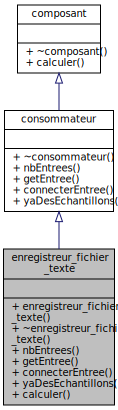
\includegraphics[width=178pt]{classenregistreur__fichier__texte__inherit__graph}
\end{center}
\end{figure}


Collaboration diagram for enregistreur\-\_\-fichier\-\_\-texte\-:
\nopagebreak
\begin{figure}[H]
\begin{center}
\leavevmode
\includegraphics[width=178pt]{classenregistreur__fichier__texte__coll__graph}
\end{center}
\end{figure}
\subsection*{Public Member Functions}
\begin{DoxyCompactItemize}
\item 
\hyperlink{classenregistreur__fichier__texte_ae421d362a8dbe086607541e97734c497}{enregistreur\-\_\-fichier\-\_\-texte} (std\-::string nf, unsigned int nbc)
\begin{DoxyCompactList}\small\item\em initialise le flux de sortie \end{DoxyCompactList}\item 
virtual \hyperlink{classenregistreur__fichier__texte_ae92b7cba4a2ffcb9055b23bfeb631ba0}{$\sim$enregistreur\-\_\-fichier\-\_\-texte} ()
\begin{DoxyCompactList}\small\item\em Destructeur virtuel. ; ferme le fichier. \end{DoxyCompactList}\item 
unsigned int \hyperlink{classenregistreur__fichier__texte_a0f686274b3cca79fba1d3c2227cd4950}{nb\-Entrees} () const 
\item 
virtual const \hyperlink{classcounted__ptr}{counted\-\_\-ptr}$<$ \hyperlink{classflot}{flot} $>$ \& \hyperlink{classenregistreur__fichier__texte_a065dcf79e74d6d7388dbb2909c0d2be2}{get\-Entree} (unsigned int numentree) const 
\item 
virtual void \hyperlink{classenregistreur__fichier__texte_a9da917c48db3891e757d971e8927dfda}{connecter\-Entree} (const \hyperlink{classcounted__ptr}{counted\-\_\-ptr}$<$ \hyperlink{classflot}{flot} $>$ \&f, unsigned int numentree)
\begin{DoxyCompactList}\small\item\em Connecte une entrée sur ce composant. \end{DoxyCompactList}\item 
virtual bool \hyperlink{classenregistreur__fichier__texte_ac412238ca34c019727aa6ddfbe9ae56e}{ya\-Des\-Echantillons} () const 
\item 
virtual void \hyperlink{classenregistreur__fichier__texte_a3c693001317b5940f3b61033c02fb2d7}{calculer} ()
\begin{DoxyCompactList}\small\item\em Effectue les calculs associes au composant. \end{DoxyCompactList}\end{DoxyCompactItemize}
\subsection*{Private Attributes}
\begin{DoxyCompactItemize}
\item 
int \hyperlink{classenregistreur__fichier__texte_a8cf1798b552aafaeaf2f163af64334e4}{m\-\_\-nb\-E}
\item 
std\-::vector$<$ \hyperlink{classcounted__ptr}{counted\-\_\-ptr}$<$ \hyperlink{classflot}{flot} $>$ $>$ \hyperlink{classenregistreur__fichier__texte_ae14bdd7eedf13e9035b72605604149c0}{m\-\_\-les\-Entrees}
\item 
std\-::string \hyperlink{classenregistreur__fichier__texte_a5cb161484890a18dd4130f59b13c0494}{m\-\_\-nom\-Fichier}
\item 
std\-::ofstream \hyperlink{classenregistreur__fichier__texte_a60a1e2e5f42a546b5065eec67720e368}{m\-\_\-flux\-Sortie}
\end{DoxyCompactItemize}


\subsection{Detailed Description}
Un consommateur qui enregistre ses entrées dans un fichier texte ; une ligne = un échantillon de chaque canal. 

\begin{DoxyAuthor}{Author}
Jean Christophe Engel, Fabrice Lamarche, University Of Rennes 1 
\end{DoxyAuthor}
\begin{DoxyDate}{Date}
23/04/2010 
\end{DoxyDate}


\subsection{Constructor \& Destructor Documentation}
\hypertarget{classenregistreur__fichier__texte_ae421d362a8dbe086607541e97734c497}{\index{enregistreur\-\_\-fichier\-\_\-texte@{enregistreur\-\_\-fichier\-\_\-texte}!enregistreur\-\_\-fichier\-\_\-texte@{enregistreur\-\_\-fichier\-\_\-texte}}
\index{enregistreur\-\_\-fichier\-\_\-texte@{enregistreur\-\_\-fichier\-\_\-texte}!enregistreur_fichier_texte@{enregistreur\-\_\-fichier\-\_\-texte}}
\subsubsection[{enregistreur\-\_\-fichier\-\_\-texte}]{\setlength{\rightskip}{0pt plus 5cm}enregistreur\-\_\-fichier\-\_\-texte\-::enregistreur\-\_\-fichier\-\_\-texte (
\begin{DoxyParamCaption}
\item[{std\-::string}]{nf, }
\item[{unsigned int}]{nbc}
\end{DoxyParamCaption}
)}}\label{classenregistreur__fichier__texte_ae421d362a8dbe086607541e97734c497}


initialise le flux de sortie 


\begin{DoxyParams}{Parameters}
{\em nf} & \-: nom du fichier de sortie \\
\hline
{\em nbc} & \-: nombre de canaux (1 = mono, 2 = stéréo) \\
\hline
\end{DoxyParams}
\hypertarget{classenregistreur__fichier__texte_ae92b7cba4a2ffcb9055b23bfeb631ba0}{\index{enregistreur\-\_\-fichier\-\_\-texte@{enregistreur\-\_\-fichier\-\_\-texte}!$\sim$enregistreur\-\_\-fichier\-\_\-texte@{$\sim$enregistreur\-\_\-fichier\-\_\-texte}}
\index{$\sim$enregistreur\-\_\-fichier\-\_\-texte@{$\sim$enregistreur\-\_\-fichier\-\_\-texte}!enregistreur_fichier_texte@{enregistreur\-\_\-fichier\-\_\-texte}}
\subsubsection[{$\sim$enregistreur\-\_\-fichier\-\_\-texte}]{\setlength{\rightskip}{0pt plus 5cm}enregistreur\-\_\-fichier\-\_\-texte\-::$\sim$enregistreur\-\_\-fichier\-\_\-texte (
\begin{DoxyParamCaption}
{}
\end{DoxyParamCaption}
)\hspace{0.3cm}{\ttfamily [virtual]}}}\label{classenregistreur__fichier__texte_ae92b7cba4a2ffcb9055b23bfeb631ba0}


Destructeur virtuel. ; ferme le fichier. 



\subsection{Member Function Documentation}
\hypertarget{classenregistreur__fichier__texte_a3c693001317b5940f3b61033c02fb2d7}{\index{enregistreur\-\_\-fichier\-\_\-texte@{enregistreur\-\_\-fichier\-\_\-texte}!calculer@{calculer}}
\index{calculer@{calculer}!enregistreur_fichier_texte@{enregistreur\-\_\-fichier\-\_\-texte}}
\subsubsection[{calculer}]{\setlength{\rightskip}{0pt plus 5cm}virtual void enregistreur\-\_\-fichier\-\_\-texte\-::calculer (
\begin{DoxyParamCaption}
{}
\end{DoxyParamCaption}
)\hspace{0.3cm}{\ttfamily [virtual]}}}\label{classenregistreur__fichier__texte_a3c693001317b5940f3b61033c02fb2d7}


Effectue les calculs associes au composant. 



Implements \hyperlink{classcomposant_a257333d140850f51be479b025ce1e540}{composant}.

\hypertarget{classenregistreur__fichier__texte_a9da917c48db3891e757d971e8927dfda}{\index{enregistreur\-\_\-fichier\-\_\-texte@{enregistreur\-\_\-fichier\-\_\-texte}!connecter\-Entree@{connecter\-Entree}}
\index{connecter\-Entree@{connecter\-Entree}!enregistreur_fichier_texte@{enregistreur\-\_\-fichier\-\_\-texte}}
\subsubsection[{connecter\-Entree}]{\setlength{\rightskip}{0pt plus 5cm}virtual void enregistreur\-\_\-fichier\-\_\-texte\-::connecter\-Entree (
\begin{DoxyParamCaption}
\item[{const {\bf counted\-\_\-ptr}$<$ {\bf flot} $>$ \&}]{f, }
\item[{unsigned int}]{numentree}
\end{DoxyParamCaption}
)\hspace{0.3cm}{\ttfamily [virtual]}}}\label{classenregistreur__fichier__texte_a9da917c48db3891e757d971e8927dfda}


Connecte une entrée sur ce composant. 


\begin{DoxyParams}{Parameters}
{\em f} & Le flot à connecter en entrée du composant. \\
\hline
{\em numentree} & Le numéro de l'entree sur laquelle connecter le flot.\\
\hline
\end{DoxyParams}
\begin{DoxyPrecond}{Precondition}
0 $<$= numentree $<$ \hyperlink{classenregistreur__fichier__texte_a0f686274b3cca79fba1d3c2227cd4950}{nb\-Entrees()} 
\end{DoxyPrecond}


Implements \hyperlink{classconsommateur_a36b438c3e6c8e71989ec30441c821062}{consommateur}.

\hypertarget{classenregistreur__fichier__texte_a065dcf79e74d6d7388dbb2909c0d2be2}{\index{enregistreur\-\_\-fichier\-\_\-texte@{enregistreur\-\_\-fichier\-\_\-texte}!get\-Entree@{get\-Entree}}
\index{get\-Entree@{get\-Entree}!enregistreur_fichier_texte@{enregistreur\-\_\-fichier\-\_\-texte}}
\subsubsection[{get\-Entree}]{\setlength{\rightskip}{0pt plus 5cm}virtual const {\bf counted\-\_\-ptr}$<${\bf flot}$>$\& enregistreur\-\_\-fichier\-\_\-texte\-::get\-Entree (
\begin{DoxyParamCaption}
\item[{unsigned int}]{numentree}
\end{DoxyParamCaption}
) const\hspace{0.3cm}{\ttfamily [virtual]}}}\label{classenregistreur__fichier__texte_a065dcf79e74d6d7388dbb2909c0d2be2}
\begin{DoxyReturn}{Returns}
L'entrée demandée. 
\end{DoxyReturn}


Implements \hyperlink{classconsommateur_ab9d91275bf6355ffa417ceb379967af2}{consommateur}.

\hypertarget{classenregistreur__fichier__texte_a0f686274b3cca79fba1d3c2227cd4950}{\index{enregistreur\-\_\-fichier\-\_\-texte@{enregistreur\-\_\-fichier\-\_\-texte}!nb\-Entrees@{nb\-Entrees}}
\index{nb\-Entrees@{nb\-Entrees}!enregistreur_fichier_texte@{enregistreur\-\_\-fichier\-\_\-texte}}
\subsubsection[{nb\-Entrees}]{\setlength{\rightskip}{0pt plus 5cm}unsigned int enregistreur\-\_\-fichier\-\_\-texte\-::nb\-Entrees (
\begin{DoxyParamCaption}
{}
\end{DoxyParamCaption}
) const\hspace{0.3cm}{\ttfamily [virtual]}}}\label{classenregistreur__fichier__texte_a0f686274b3cca79fba1d3c2227cd4950}
\begin{DoxyReturn}{Returns}
Le nombre d'entrees du composant. 
\end{DoxyReturn}


Implements \hyperlink{classconsommateur_aa06328f3002f14b5ff83e393e7e4761a}{consommateur}.

\hypertarget{classenregistreur__fichier__texte_ac412238ca34c019727aa6ddfbe9ae56e}{\index{enregistreur\-\_\-fichier\-\_\-texte@{enregistreur\-\_\-fichier\-\_\-texte}!ya\-Des\-Echantillons@{ya\-Des\-Echantillons}}
\index{ya\-Des\-Echantillons@{ya\-Des\-Echantillons}!enregistreur_fichier_texte@{enregistreur\-\_\-fichier\-\_\-texte}}
\subsubsection[{ya\-Des\-Echantillons}]{\setlength{\rightskip}{0pt plus 5cm}virtual bool enregistreur\-\_\-fichier\-\_\-texte\-::ya\-Des\-Echantillons (
\begin{DoxyParamCaption}
{}
\end{DoxyParamCaption}
) const\hspace{0.3cm}{\ttfamily [virtual]}}}\label{classenregistreur__fichier__texte_ac412238ca34c019727aa6ddfbe9ae56e}
\begin{DoxyReturn}{Returns}
Vrai si chaque entrée possède au moins un échantillon. 
\end{DoxyReturn}


Implements \hyperlink{classconsommateur_a8622fe9e8e5baa1a7b152fce88b8be89}{consommateur}.



\subsection{Member Data Documentation}
\hypertarget{classenregistreur__fichier__texte_a60a1e2e5f42a546b5065eec67720e368}{\index{enregistreur\-\_\-fichier\-\_\-texte@{enregistreur\-\_\-fichier\-\_\-texte}!m\-\_\-flux\-Sortie@{m\-\_\-flux\-Sortie}}
\index{m\-\_\-flux\-Sortie@{m\-\_\-flux\-Sortie}!enregistreur_fichier_texte@{enregistreur\-\_\-fichier\-\_\-texte}}
\subsubsection[{m\-\_\-flux\-Sortie}]{\setlength{\rightskip}{0pt plus 5cm}std\-::ofstream enregistreur\-\_\-fichier\-\_\-texte\-::m\-\_\-flux\-Sortie\hspace{0.3cm}{\ttfamily [private]}}}\label{classenregistreur__fichier__texte_a60a1e2e5f42a546b5065eec67720e368}
\hypertarget{classenregistreur__fichier__texte_ae14bdd7eedf13e9035b72605604149c0}{\index{enregistreur\-\_\-fichier\-\_\-texte@{enregistreur\-\_\-fichier\-\_\-texte}!m\-\_\-les\-Entrees@{m\-\_\-les\-Entrees}}
\index{m\-\_\-les\-Entrees@{m\-\_\-les\-Entrees}!enregistreur_fichier_texte@{enregistreur\-\_\-fichier\-\_\-texte}}
\subsubsection[{m\-\_\-les\-Entrees}]{\setlength{\rightskip}{0pt plus 5cm}std\-::vector$<${\bf counted\-\_\-ptr}$<${\bf flot}$>$ $>$ enregistreur\-\_\-fichier\-\_\-texte\-::m\-\_\-les\-Entrees\hspace{0.3cm}{\ttfamily [private]}}}\label{classenregistreur__fichier__texte_ae14bdd7eedf13e9035b72605604149c0}
\hypertarget{classenregistreur__fichier__texte_a8cf1798b552aafaeaf2f163af64334e4}{\index{enregistreur\-\_\-fichier\-\_\-texte@{enregistreur\-\_\-fichier\-\_\-texte}!m\-\_\-nb\-E@{m\-\_\-nb\-E}}
\index{m\-\_\-nb\-E@{m\-\_\-nb\-E}!enregistreur_fichier_texte@{enregistreur\-\_\-fichier\-\_\-texte}}
\subsubsection[{m\-\_\-nb\-E}]{\setlength{\rightskip}{0pt plus 5cm}int enregistreur\-\_\-fichier\-\_\-texte\-::m\-\_\-nb\-E\hspace{0.3cm}{\ttfamily [private]}}}\label{classenregistreur__fichier__texte_a8cf1798b552aafaeaf2f163af64334e4}
\hypertarget{classenregistreur__fichier__texte_a5cb161484890a18dd4130f59b13c0494}{\index{enregistreur\-\_\-fichier\-\_\-texte@{enregistreur\-\_\-fichier\-\_\-texte}!m\-\_\-nom\-Fichier@{m\-\_\-nom\-Fichier}}
\index{m\-\_\-nom\-Fichier@{m\-\_\-nom\-Fichier}!enregistreur_fichier_texte@{enregistreur\-\_\-fichier\-\_\-texte}}
\subsubsection[{m\-\_\-nom\-Fichier}]{\setlength{\rightskip}{0pt plus 5cm}std\-::string enregistreur\-\_\-fichier\-\_\-texte\-::m\-\_\-nom\-Fichier\hspace{0.3cm}{\ttfamily [private]}}}\label{classenregistreur__fichier__texte_a5cb161484890a18dd4130f59b13c0494}


The documentation for this class was generated from the following file\-:\begin{DoxyCompactItemize}
\item 
include/\hyperlink{enregistreur__fichier__texte_8h}{enregistreur\-\_\-fichier\-\_\-texte.\-h}\end{DoxyCompactItemize}

\hypertarget{classfile__reader}{\section{file\-\_\-reader Class Reference}
\label{classfile__reader}\index{file\-\_\-reader@{file\-\_\-reader}}
}


{\ttfamily \#include $<$file\-\_\-reader.\-h$>$}



Inheritance diagram for file\-\_\-reader\-:
\nopagebreak
\begin{figure}[H]
\begin{center}
\leavevmode
\includegraphics[width=168pt]{classfile__reader__inherit__graph}
\end{center}
\end{figure}


Collaboration diagram for file\-\_\-reader\-:
\nopagebreak
\begin{figure}[H]
\begin{center}
\leavevmode
\includegraphics[width=168pt]{classfile__reader__coll__graph}
\end{center}
\end{figure}
\subsection*{Public Member Functions}
\begin{DoxyCompactItemize}
\item 
\hyperlink{classfile__reader_ad044fe1536ebee72e77fdd2973300dda}{file\-\_\-reader} (char $\ast$, unsigned int)
\item 
virtual \hyperlink{classfile__reader_a86aa8bf64bad02300e177401f8da6aee}{$\sim$file\-\_\-reader} ()
\item 
virtual void \hyperlink{classfile__reader_ac63890e9fbb85cda005efbce47f83648}{calculer} ()
\begin{DoxyCompactList}\small\item\em Effectue les calculs associes au composant. \end{DoxyCompactList}\end{DoxyCompactItemize}
\subsection*{Private Attributes}
\begin{DoxyCompactItemize}
\item 
std\-::ifstream \hyperlink{classfile__reader_aa7f6d7d6b00fe7e0524db94b2a279c8c}{m\-\_\-handle}
\item 
unsigned int \hyperlink{classfile__reader_a3dfaa67bb8ea591695eb1eecfdea4cde}{m\-\_\-canals}
\end{DoxyCompactItemize}
\subsection*{Additional Inherited Members}


\subsection{Constructor \& Destructor Documentation}
\hypertarget{classfile__reader_ad044fe1536ebee72e77fdd2973300dda}{\index{file\-\_\-reader@{file\-\_\-reader}!file\-\_\-reader@{file\-\_\-reader}}
\index{file\-\_\-reader@{file\-\_\-reader}!file_reader@{file\-\_\-reader}}
\subsubsection[{file\-\_\-reader}]{\setlength{\rightskip}{0pt plus 5cm}file\-\_\-reader\-::file\-\_\-reader (
\begin{DoxyParamCaption}
\item[{char $\ast$}]{filename, }
\item[{unsigned int}]{canals}
\end{DoxyParamCaption}
)}}\label{classfile__reader_ad044fe1536ebee72e77fdd2973300dda}
Lit un fichier et fournit son contenu sous forme de flot filename est le nom du fichier à lire canals est le nombre de canaux du fichier (1\-: mono, 2\-: stereo) \hypertarget{classfile__reader_a86aa8bf64bad02300e177401f8da6aee}{\index{file\-\_\-reader@{file\-\_\-reader}!$\sim$file\-\_\-reader@{$\sim$file\-\_\-reader}}
\index{$\sim$file\-\_\-reader@{$\sim$file\-\_\-reader}!file_reader@{file\-\_\-reader}}
\subsubsection[{$\sim$file\-\_\-reader}]{\setlength{\rightskip}{0pt plus 5cm}virtual file\-\_\-reader\-::$\sim$file\-\_\-reader (
\begin{DoxyParamCaption}
{}
\end{DoxyParamCaption}
)\hspace{0.3cm}{\ttfamily [inline]}, {\ttfamily [virtual]}}}\label{classfile__reader_a86aa8bf64bad02300e177401f8da6aee}


\subsection{Member Function Documentation}
\hypertarget{classfile__reader_ac63890e9fbb85cda005efbce47f83648}{\index{file\-\_\-reader@{file\-\_\-reader}!calculer@{calculer}}
\index{calculer@{calculer}!file_reader@{file\-\_\-reader}}
\subsubsection[{calculer}]{\setlength{\rightskip}{0pt plus 5cm}void file\-\_\-reader\-::calculer (
\begin{DoxyParamCaption}
{}
\end{DoxyParamCaption}
)\hspace{0.3cm}{\ttfamily [virtual]}}}\label{classfile__reader_ac63890e9fbb85cda005efbce47f83648}


Effectue les calculs associes au composant. 



Implements \hyperlink{classproducteur__base_af1e171c9e69b0998d5124c7389737f82}{producteur\-\_\-base}.



\subsection{Member Data Documentation}
\hypertarget{classfile__reader_a3dfaa67bb8ea591695eb1eecfdea4cde}{\index{file\-\_\-reader@{file\-\_\-reader}!m\-\_\-canals@{m\-\_\-canals}}
\index{m\-\_\-canals@{m\-\_\-canals}!file_reader@{file\-\_\-reader}}
\subsubsection[{m\-\_\-canals}]{\setlength{\rightskip}{0pt plus 5cm}unsigned int file\-\_\-reader\-::m\-\_\-canals\hspace{0.3cm}{\ttfamily [private]}}}\label{classfile__reader_a3dfaa67bb8ea591695eb1eecfdea4cde}
Nombre de canaux dans ce fichier \hypertarget{classfile__reader_aa7f6d7d6b00fe7e0524db94b2a279c8c}{\index{file\-\_\-reader@{file\-\_\-reader}!m\-\_\-handle@{m\-\_\-handle}}
\index{m\-\_\-handle@{m\-\_\-handle}!file_reader@{file\-\_\-reader}}
\subsubsection[{m\-\_\-handle}]{\setlength{\rightskip}{0pt plus 5cm}std\-::ifstream file\-\_\-reader\-::m\-\_\-handle\hspace{0.3cm}{\ttfamily [private]}}}\label{classfile__reader_aa7f6d7d6b00fe7e0524db94b2a279c8c}
Handle vers le fichier à lire 

The documentation for this class was generated from the following files\-:\begin{DoxyCompactItemize}
\item 
src/\hyperlink{file__reader_8h}{file\-\_\-reader.\-h}\item 
src/\hyperlink{file__reader_8cpp}{file\-\_\-reader.\-cpp}\end{DoxyCompactItemize}

\hypertarget{classfiltre}{\section{filtre Class Reference}
\label{classfiltre}\index{filtre@{filtre}}
}


Interface associée à un filtre sonore. Ce filtre est considéré comme un producteur / consommateur d'échantillons sonores. Il possède donc des entrées et des sorties.  




{\ttfamily \#include $<$filtre.\-h$>$}



Inheritance diagram for filtre\-:
\nopagebreak
\begin{figure}[H]
\begin{center}
\leavevmode
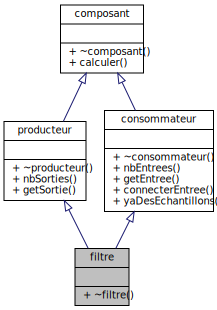
\includegraphics[width=350pt]{classfiltre__inherit__graph}
\end{center}
\end{figure}


Collaboration diagram for filtre\-:
\nopagebreak
\begin{figure}[H]
\begin{center}
\leavevmode
\includegraphics[width=241pt]{classfiltre__coll__graph}
\end{center}
\end{figure}
\subsection*{Public Member Functions}
\begin{DoxyCompactItemize}
\item 
virtual \hyperlink{classfiltre_a0f86c791e07725dd2e7b1147b7592b13}{$\sim$filtre} ()
\begin{DoxyCompactList}\small\item\em Destructeur virtuel. \end{DoxyCompactList}\end{DoxyCompactItemize}


\subsection{Detailed Description}
Interface associée à un filtre sonore. Ce filtre est considéré comme un producteur / consommateur d'échantillons sonores. Il possède donc des entrées et des sorties. 

\begin{DoxyAuthor}{Author}
Jean Christophe Engel, Fabrice Lamarche, University Of Rennes 1 
\end{DoxyAuthor}
\begin{DoxyDate}{Date}
23/04/2010 
\end{DoxyDate}


\subsection{Constructor \& Destructor Documentation}
\hypertarget{classfiltre_a0f86c791e07725dd2e7b1147b7592b13}{\index{filtre@{filtre}!$\sim$filtre@{$\sim$filtre}}
\index{$\sim$filtre@{$\sim$filtre}!filtre@{filtre}}
\subsubsection[{$\sim$filtre}]{\setlength{\rightskip}{0pt plus 5cm}filtre\-::$\sim$filtre (
\begin{DoxyParamCaption}
{}
\end{DoxyParamCaption}
)\hspace{0.3cm}{\ttfamily [inline]}, {\ttfamily [virtual]}}}\label{classfiltre_a0f86c791e07725dd2e7b1147b7592b13}


Destructeur virtuel. 



The documentation for this class was generated from the following file\-:\begin{DoxyCompactItemize}
\item 
include/\hyperlink{filtre_8h}{filtre.\-h}\end{DoxyCompactItemize}

\hypertarget{classfiltre__base}{\section{filtre\-\_\-base Class Reference}
\label{classfiltre__base}\index{filtre\-\_\-base@{filtre\-\_\-base}}
}


{\ttfamily \#include $<$filtre\-\_\-base.\-h$>$}



Inheritance diagram for filtre\-\_\-base\-:
\nopagebreak
\begin{figure}[H]
\begin{center}
\leavevmode
\includegraphics[width=350pt]{classfiltre__base__inherit__graph}
\end{center}
\end{figure}


Collaboration diagram for filtre\-\_\-base\-:
\nopagebreak
\begin{figure}[H]
\begin{center}
\leavevmode
\includegraphics[width=346pt]{classfiltre__base__coll__graph}
\end{center}
\end{figure}
\subsection*{Public Member Functions}
\begin{DoxyCompactItemize}
\item 
\hyperlink{classfiltre__base_ac193f1692a2e199666ac7343cb17dde9}{filtre\-\_\-base} (unsigned int, unsigned int)
\item 
virtual \hyperlink{classfiltre__base_a85891015e2bd3b98eec0af2ce3f03ed3}{$\sim$filtre\-\_\-base} ()
\item 
virtual void \hyperlink{classfiltre__base_ad06f5db1f851e5ad8655c9d8927cf347}{calculer} ()=0
\begin{DoxyCompactList}\small\item\em Effectue les calculs associes au composant. \end{DoxyCompactList}\end{DoxyCompactItemize}
\subsection*{Additional Inherited Members}


\subsection{Constructor \& Destructor Documentation}
\hypertarget{classfiltre__base_ac193f1692a2e199666ac7343cb17dde9}{\index{filtre\-\_\-base@{filtre\-\_\-base}!filtre\-\_\-base@{filtre\-\_\-base}}
\index{filtre\-\_\-base@{filtre\-\_\-base}!filtre_base@{filtre\-\_\-base}}
\subsubsection[{filtre\-\_\-base}]{\setlength{\rightskip}{0pt plus 5cm}filtre\-\_\-base\-::filtre\-\_\-base (
\begin{DoxyParamCaption}
\item[{unsigned int}]{in, }
\item[{unsigned int}]{out}
\end{DoxyParamCaption}
)}}\label{classfiltre__base_ac193f1692a2e199666ac7343cb17dde9}
Filtre de base (à la fois producteur et consommateur) \hypertarget{classfiltre__base_a85891015e2bd3b98eec0af2ce3f03ed3}{\index{filtre\-\_\-base@{filtre\-\_\-base}!$\sim$filtre\-\_\-base@{$\sim$filtre\-\_\-base}}
\index{$\sim$filtre\-\_\-base@{$\sim$filtre\-\_\-base}!filtre_base@{filtre\-\_\-base}}
\subsubsection[{$\sim$filtre\-\_\-base}]{\setlength{\rightskip}{0pt plus 5cm}virtual filtre\-\_\-base\-::$\sim$filtre\-\_\-base (
\begin{DoxyParamCaption}
{}
\end{DoxyParamCaption}
)\hspace{0.3cm}{\ttfamily [inline]}, {\ttfamily [virtual]}}}\label{classfiltre__base_a85891015e2bd3b98eec0af2ce3f03ed3}


\subsection{Member Function Documentation}
\hypertarget{classfiltre__base_ad06f5db1f851e5ad8655c9d8927cf347}{\index{filtre\-\_\-base@{filtre\-\_\-base}!calculer@{calculer}}
\index{calculer@{calculer}!filtre_base@{filtre\-\_\-base}}
\subsubsection[{calculer}]{\setlength{\rightskip}{0pt plus 5cm}virtual void filtre\-\_\-base\-::calculer (
\begin{DoxyParamCaption}
{}
\end{DoxyParamCaption}
)\hspace{0.3cm}{\ttfamily [pure virtual]}}}\label{classfiltre__base_ad06f5db1f851e5ad8655c9d8927cf347}


Effectue les calculs associes au composant. 



Implements \hyperlink{classproducteur__base_af1e171c9e69b0998d5124c7389737f82}{producteur\-\_\-base}.



Implemented in \hyperlink{classoperation__binaire_a2ecfa3c6c05006c5c1bc285281bc6f3a}{operation\-\_\-binaire$<$ T $>$}, \hyperlink{classfiltre__compose_a6fd1598c04300da43989af4f87a37aba}{filtre\-\_\-compose}, \hyperlink{classvolume_aab5a1f0490ea8b5826db6edd78e90f1d}{volume}, and \hyperlink{classmultiplicateur_ab22f15668247a10a35f027bd503f2442}{multiplicateur}.



The documentation for this class was generated from the following files\-:\begin{DoxyCompactItemize}
\item 
src/\hyperlink{filtre__base_8h}{filtre\-\_\-base.\-h}\item 
src/\hyperlink{filtre__base_8cpp}{filtre\-\_\-base.\-cpp}\end{DoxyCompactItemize}

\hypertarget{classfiltre__compose}{\section{filtre\-\_\-compose Class Reference}
\label{classfiltre__compose}\index{filtre\-\_\-compose@{filtre\-\_\-compose}}
}


{\ttfamily \#include $<$filtre\-\_\-compose.\-h$>$}



Inheritance diagram for filtre\-\_\-compose\-:
\nopagebreak
\begin{figure}[H]
\begin{center}
\leavevmode
\includegraphics[width=346pt]{classfiltre__compose__inherit__graph}
\end{center}
\end{figure}


Collaboration diagram for filtre\-\_\-compose\-:
\nopagebreak
\begin{figure}[H]
\begin{center}
\leavevmode
\includegraphics[width=346pt]{classfiltre__compose__coll__graph}
\end{center}
\end{figure}
\subsection*{Public Member Functions}
\begin{DoxyCompactItemize}
\item 
\hyperlink{classfiltre__compose_a7e3d377ce43f6dabc6709f57b9aaf4b6}{filtre\-\_\-compose} (unsigned int, unsigned int)
\item 
virtual void \hyperlink{classfiltre__compose_a7ac6503a5391d0f633203c0b094a6e9f}{connecter\-Composants} (\hyperlink{classcounted__ptr}{counted\-\_\-ptr}$<$ \hyperlink{classproducteur}{producteur} $>$, unsigned int, \hyperlink{classcounted__ptr}{counted\-\_\-ptr}$<$ \hyperlink{classconsommateur}{consommateur} $>$, unsigned int)
\item 
void \hyperlink{classfiltre__compose_a8b205525be2ba74557c5284ed72406a2}{ajouter\-Composant} (\hyperlink{classcounted__ptr}{counted\-\_\-ptr}$<$ \hyperlink{classcomposant}{composant} $>$)
\item 
void \hyperlink{classfiltre__compose_ad30c331895f65539dad8e62ed5fcfc04}{connecter\-Sortie\-Interne} (\hyperlink{classcounted__ptr}{counted\-\_\-ptr}$<$ \hyperlink{classproducteur__base}{producteur\-\_\-base} $>$, unsigned int, unsigned int)
\item 
void \hyperlink{classfiltre__compose_ad9c8d2f971d2a71859fad598d11e180b}{connecter\-Entree\-Interne} (\hyperlink{classcounted__ptr}{counted\-\_\-ptr}$<$ \hyperlink{classconsommateur__base}{consommateur\-\_\-base} $>$, unsigned int, unsigned int)
\item 
void \hyperlink{classfiltre__compose_aaf4dc84a41236fb7f462d6eba569baf1}{connecter\-Entree} (const \hyperlink{classcounted__ptr}{counted\-\_\-ptr}$<$ \hyperlink{classflot}{flot} $>$ \&, unsigned int)
\item 
virtual void \hyperlink{classfiltre__compose_a6fd1598c04300da43989af4f87a37aba}{calculer} ()
\end{DoxyCompactItemize}
\subsection*{Private Attributes}
\begin{DoxyCompactItemize}
\item 
std\-::vector$<$ \hyperlink{classcounted__ptr}{counted\-\_\-ptr}\\*
$<$ \hyperlink{classcomposant}{composant} $>$ $>$ \hyperlink{classfiltre__compose_ae857e33daea1b9afa3689322241dac33}{m\-\_\-filters}
\item 
std\-::map$<$ unsigned int, \\*
std\-::pair$<$ \hyperlink{classcounted__ptr}{counted\-\_\-ptr}\\*
$<$ \hyperlink{classconsommateur}{consommateur} $>$, unsigned int $>$ $>$ \hyperlink{classfiltre__compose_ab0a900380de582219751e3451104cfa7}{m\-\_\-dict}
\end{DoxyCompactItemize}
\subsection*{Additional Inherited Members}


\subsection{Constructor \& Destructor Documentation}
\hypertarget{classfiltre__compose_a7e3d377ce43f6dabc6709f57b9aaf4b6}{\index{filtre\-\_\-compose@{filtre\-\_\-compose}!filtre\-\_\-compose@{filtre\-\_\-compose}}
\index{filtre\-\_\-compose@{filtre\-\_\-compose}!filtre_compose@{filtre\-\_\-compose}}
\subsubsection[{filtre\-\_\-compose}]{\setlength{\rightskip}{0pt plus 5cm}filtre\-\_\-compose\-::filtre\-\_\-compose (
\begin{DoxyParamCaption}
\item[{unsigned int}]{in, }
\item[{unsigned int}]{out}
\end{DoxyParamCaption}
)}}\label{classfiltre__compose_a7e3d377ce43f6dabc6709f57b9aaf4b6}
Filtre composé de plusieurs composants reliés les uns les autres. in représente le nombre d'entrées out représente le nombre de sorties 

\subsection{Member Function Documentation}
\hypertarget{classfiltre__compose_a8b205525be2ba74557c5284ed72406a2}{\index{filtre\-\_\-compose@{filtre\-\_\-compose}!ajouter\-Composant@{ajouter\-Composant}}
\index{ajouter\-Composant@{ajouter\-Composant}!filtre_compose@{filtre\-\_\-compose}}
\subsubsection[{ajouter\-Composant}]{\setlength{\rightskip}{0pt plus 5cm}void filtre\-\_\-compose\-::ajouter\-Composant (
\begin{DoxyParamCaption}
\item[{{\bf counted\-\_\-ptr}$<$ {\bf composant} $>$}]{composant}
\end{DoxyParamCaption}
)}}\label{classfiltre__compose_a8b205525be2ba74557c5284ed72406a2}
Ajoute un composant dans le filtre \hypertarget{classfiltre__compose_a6fd1598c04300da43989af4f87a37aba}{\index{filtre\-\_\-compose@{filtre\-\_\-compose}!calculer@{calculer}}
\index{calculer@{calculer}!filtre_compose@{filtre\-\_\-compose}}
\subsubsection[{calculer}]{\setlength{\rightskip}{0pt plus 5cm}void filtre\-\_\-compose\-::calculer (
\begin{DoxyParamCaption}
{}
\end{DoxyParamCaption}
)\hspace{0.3cm}{\ttfamily [virtual]}}}\label{classfiltre__compose_a6fd1598c04300da43989af4f87a37aba}
Calcule les valeurs à sortir en traversant tous les composants et en appliquand les filtres. 

Implements \hyperlink{classfiltre__base_ad06f5db1f851e5ad8655c9d8927cf347}{filtre\-\_\-base}.

\hypertarget{classfiltre__compose_a7ac6503a5391d0f633203c0b094a6e9f}{\index{filtre\-\_\-compose@{filtre\-\_\-compose}!connecter\-Composants@{connecter\-Composants}}
\index{connecter\-Composants@{connecter\-Composants}!filtre_compose@{filtre\-\_\-compose}}
\subsubsection[{connecter\-Composants}]{\setlength{\rightskip}{0pt plus 5cm}void filtre\-\_\-compose\-::connecter\-Composants (
\begin{DoxyParamCaption}
\item[{{\bf counted\-\_\-ptr}$<$ {\bf producteur} $>$}]{prod, }
\item[{unsigned int}]{out\-Prod, }
\item[{{\bf counted\-\_\-ptr}$<$ {\bf consommateur} $>$}]{cons, }
\item[{unsigned int}]{cons\-Prod}
\end{DoxyParamCaption}
)\hspace{0.3cm}{\ttfamily [virtual]}}}\label{classfiltre__compose_a7ac6503a5391d0f633203c0b094a6e9f}
Connecte deux composants internes ensemble. \hypertarget{classfiltre__compose_aaf4dc84a41236fb7f462d6eba569baf1}{\index{filtre\-\_\-compose@{filtre\-\_\-compose}!connecter\-Entree@{connecter\-Entree}}
\index{connecter\-Entree@{connecter\-Entree}!filtre_compose@{filtre\-\_\-compose}}
\subsubsection[{connecter\-Entree}]{\setlength{\rightskip}{0pt plus 5cm}void filtre\-\_\-compose\-::connecter\-Entree (
\begin{DoxyParamCaption}
\item[{const {\bf counted\-\_\-ptr}$<$ {\bf flot} $>$ \&}]{cmp, }
\item[{unsigned int}]{in}
\end{DoxyParamCaption}
)\hspace{0.3cm}{\ttfamily [virtual]}}}\label{classfiltre__compose_aaf4dc84a41236fb7f462d6eba569baf1}
Connecte un flot à une entrée du filtre 

Reimplemented from \hyperlink{classconsommateur__base_a273d1899ba7e05e8651b4cca6aa35b1d}{consommateur\-\_\-base}.

\hypertarget{classfiltre__compose_ad9c8d2f971d2a71859fad598d11e180b}{\index{filtre\-\_\-compose@{filtre\-\_\-compose}!connecter\-Entree\-Interne@{connecter\-Entree\-Interne}}
\index{connecter\-Entree\-Interne@{connecter\-Entree\-Interne}!filtre_compose@{filtre\-\_\-compose}}
\subsubsection[{connecter\-Entree\-Interne}]{\setlength{\rightskip}{0pt plus 5cm}void filtre\-\_\-compose\-::connecter\-Entree\-Interne (
\begin{DoxyParamCaption}
\item[{{\bf counted\-\_\-ptr}$<$ {\bf consommateur\-\_\-base} $>$}]{cmp, }
\item[{unsigned int}]{in, }
\item[{unsigned int}]{in\-Cmp}
\end{DoxyParamCaption}
)}}\label{classfiltre__compose_ad9c8d2f971d2a71859fad598d11e180b}
Connecte une entrée d'un composant interne à une entrée du filtre cmp est le composant interne in l'entrée du filtre in\-Cmp l'entrée du composant \hypertarget{classfiltre__compose_ad30c331895f65539dad8e62ed5fcfc04}{\index{filtre\-\_\-compose@{filtre\-\_\-compose}!connecter\-Sortie\-Interne@{connecter\-Sortie\-Interne}}
\index{connecter\-Sortie\-Interne@{connecter\-Sortie\-Interne}!filtre_compose@{filtre\-\_\-compose}}
\subsubsection[{connecter\-Sortie\-Interne}]{\setlength{\rightskip}{0pt plus 5cm}void filtre\-\_\-compose\-::connecter\-Sortie\-Interne (
\begin{DoxyParamCaption}
\item[{{\bf counted\-\_\-ptr}$<$ {\bf producteur\-\_\-base} $>$}]{cmp, }
\item[{unsigned int}]{out, }
\item[{unsigned int}]{out\-Cmp}
\end{DoxyParamCaption}
)}}\label{classfiltre__compose_ad30c331895f65539dad8e62ed5fcfc04}
Connecte une sortie d'un composant externe à une sortie du filtre cmp est le composant externe in la sortie du filtre in\-Cmp la sortie du composant 

\subsection{Member Data Documentation}
\hypertarget{classfiltre__compose_ab0a900380de582219751e3451104cfa7}{\index{filtre\-\_\-compose@{filtre\-\_\-compose}!m\-\_\-dict@{m\-\_\-dict}}
\index{m\-\_\-dict@{m\-\_\-dict}!filtre_compose@{filtre\-\_\-compose}}
\subsubsection[{m\-\_\-dict}]{\setlength{\rightskip}{0pt plus 5cm}std\-::map$<$unsigned int, std\-::pair$<${\bf counted\-\_\-ptr}$<${\bf consommateur}$>$, unsigned int$>$ $>$ filtre\-\_\-compose\-::m\-\_\-dict\hspace{0.3cm}{\ttfamily [private]}}}\label{classfiltre__compose_ab0a900380de582219751e3451104cfa7}
Dictionnaire reliant un numéro d'entrée à une entrée d'un composant \hypertarget{classfiltre__compose_ae857e33daea1b9afa3689322241dac33}{\index{filtre\-\_\-compose@{filtre\-\_\-compose}!m\-\_\-filters@{m\-\_\-filters}}
\index{m\-\_\-filters@{m\-\_\-filters}!filtre_compose@{filtre\-\_\-compose}}
\subsubsection[{m\-\_\-filters}]{\setlength{\rightskip}{0pt plus 5cm}std\-::vector$<${\bf counted\-\_\-ptr}$<${\bf composant}$>$ $>$ filtre\-\_\-compose\-::m\-\_\-filters\hspace{0.3cm}{\ttfamily [private]}}}\label{classfiltre__compose_ae857e33daea1b9afa3689322241dac33}
Liste des composants 

The documentation for this class was generated from the following files\-:\begin{DoxyCompactItemize}
\item 
src/\hyperlink{filtre__compose_8h}{filtre\-\_\-compose.\-h}\item 
src/\hyperlink{filtre__compose_8cpp}{filtre\-\_\-compose.\-cpp}\end{DoxyCompactItemize}

\hypertarget{classflot}{\section{flot Class Reference}
\label{classflot}\index{flot@{flot}}
}


Interface associee a un flot de donnees reliant deux composants du systeme.  




{\ttfamily \#include $<$flot.\-h$>$}



Inheritance diagram for flot\-:
\nopagebreak
\begin{figure}[H]
\begin{center}
\leavevmode
\includegraphics[width=130pt]{classflot__inherit__graph}
\end{center}
\end{figure}
\subsection*{Public Member Functions}
\begin{DoxyCompactItemize}
\item 
virtual \hyperlink{classflot_ae73ea3f5f51ae0994305f85fba4f80da}{$\sim$flot} ()
\begin{DoxyCompactList}\small\item\em Destructeur virtuel. \end{DoxyCompactList}\item 
virtual void \hyperlink{classflot_a324d696c55f5b0f0b036f8069ffe7911}{inserer} (double echantillon)=0
\begin{DoxyCompactList}\small\item\em Insertion d'un echantillon dans le flot. \end{DoxyCompactList}\item 
virtual double \hyperlink{classflot_a84b9830b712c4c96f052b04883c4fa80}{extraire} ()=0
\begin{DoxyCompactList}\small\item\em Extraction de l'echantillon situe en tete du flot. \end{DoxyCompactList}\item 
virtual bool \hyperlink{classflot_aa1dc8b1beedc87daedd4fc0f5354cbb6}{vide} () const =0
\begin{DoxyCompactList}\small\item\em Permet de savoir si le flot est vide ou non. \end{DoxyCompactList}\end{DoxyCompactItemize}


\subsection{Detailed Description}
Interface associee a un flot de donnees reliant deux composants du systeme. 

\begin{DoxyAuthor}{Author}
Jean Christophe Engel, Fabrice Lamarche, University Of Rennes 1 
\end{DoxyAuthor}
\begin{DoxyDate}{Date}
23/04/2010 
\end{DoxyDate}


\subsection{Constructor \& Destructor Documentation}
\hypertarget{classflot_ae73ea3f5f51ae0994305f85fba4f80da}{\index{flot@{flot}!$\sim$flot@{$\sim$flot}}
\index{$\sim$flot@{$\sim$flot}!flot@{flot}}
\subsubsection[{$\sim$flot}]{\setlength{\rightskip}{0pt plus 5cm}flot\-::$\sim$flot (
\begin{DoxyParamCaption}
{}
\end{DoxyParamCaption}
)\hspace{0.3cm}{\ttfamily [inline]}, {\ttfamily [virtual]}}}\label{classflot_ae73ea3f5f51ae0994305f85fba4f80da}


Destructeur virtuel. 



\subsection{Member Function Documentation}
\hypertarget{classflot_a84b9830b712c4c96f052b04883c4fa80}{\index{flot@{flot}!extraire@{extraire}}
\index{extraire@{extraire}!flot@{flot}}
\subsubsection[{extraire}]{\setlength{\rightskip}{0pt plus 5cm}double flot\-::extraire (
\begin{DoxyParamCaption}
{}
\end{DoxyParamCaption}
)\hspace{0.3cm}{\ttfamily [pure virtual]}}}\label{classflot_a84b9830b712c4c96f052b04883c4fa80}


Extraction de l'echantillon situe en tete du flot. 

\begin{DoxyPrecond}{Precondition}
!vide() 
\end{DoxyPrecond}
\begin{DoxyReturn}{Returns}
L'echantillon en tete de flot. 
\end{DoxyReturn}


Implemented in \hyperlink{classimp__flot_ab3abbb6e555cbc62061bd6bcfda0050c}{imp\-\_\-flot}.

\hypertarget{classflot_a324d696c55f5b0f0b036f8069ffe7911}{\index{flot@{flot}!inserer@{inserer}}
\index{inserer@{inserer}!flot@{flot}}
\subsubsection[{inserer}]{\setlength{\rightskip}{0pt plus 5cm}void flot\-::inserer (
\begin{DoxyParamCaption}
\item[{double}]{echantillon}
\end{DoxyParamCaption}
)\hspace{0.3cm}{\ttfamily [pure virtual]}}}\label{classflot_a324d696c55f5b0f0b036f8069ffe7911}


Insertion d'un echantillon dans le flot. 


\begin{DoxyParams}{Parameters}
{\em echantillon} & L'echantillon a inserer dans le flot. \\
\hline
\end{DoxyParams}


Implemented in \hyperlink{classimp__flot_ae8d3f81777edab07b0dccacc630e16e5}{imp\-\_\-flot}.

\hypertarget{classflot_aa1dc8b1beedc87daedd4fc0f5354cbb6}{\index{flot@{flot}!vide@{vide}}
\index{vide@{vide}!flot@{flot}}
\subsubsection[{vide}]{\setlength{\rightskip}{0pt plus 5cm}bool flot\-::vide (
\begin{DoxyParamCaption}
{}
\end{DoxyParamCaption}
) const\hspace{0.3cm}{\ttfamily [pure virtual]}}}\label{classflot_aa1dc8b1beedc87daedd4fc0f5354cbb6}


Permet de savoir si le flot est vide ou non. 

\begin{DoxyReturn}{Returns}
Vrai si le flot est vide, faux sinon. 
\end{DoxyReturn}


Implemented in \hyperlink{classimp__flot_a3757d33b984840955902ce982719e0f3}{imp\-\_\-flot}.



The documentation for this class was generated from the following file\-:\begin{DoxyCompactItemize}
\item 
include/\hyperlink{flot_8h}{flot.\-h}\end{DoxyCompactItemize}

\hypertarget{classharmonique}{\section{harmonique Class Reference}
\label{classharmonique}\index{harmonique@{harmonique}}
}


{\ttfamily \#include $<$harmonique.\-h$>$}



Inheritance diagram for harmonique\-:
\nopagebreak
\begin{figure}[H]
\begin{center}
\leavevmode
\includegraphics[width=168pt]{classharmonique__inherit__graph}
\end{center}
\end{figure}


Collaboration diagram for harmonique\-:
\nopagebreak
\begin{figure}[H]
\begin{center}
\leavevmode
\includegraphics[width=168pt]{classharmonique__coll__graph}
\end{center}
\end{figure}
\subsection*{Public Member Functions}
\begin{DoxyCompactItemize}
\item 
\hyperlink{classharmonique_ac4326b55d526129329391f36991e2f73}{harmonique} (double)
\item 
virtual \hyperlink{classharmonique_a48a057f7ba6e8ff4e443c15da0cd2019}{$\sim$harmonique} ()
\item 
virtual void \hyperlink{classharmonique_a4dbd729dfa443204d9834effbb63d816}{calculer} ()
\end{DoxyCompactItemize}
\subsection*{Private Attributes}
\begin{DoxyCompactItemize}
\item 
double \hyperlink{classharmonique_a8f9a721707c36033703863f22d6b70a8}{m\-\_\-freq}
\item 
double \hyperlink{classharmonique_a2ba9d8b0702651bbbf67d4d7f7316c3e}{m\-\_\-dephase}
\item 
int \hyperlink{classharmonique_a648d5e64e0e8b8a5c9d4af4146ad93ae}{m\-\_\-sample\-\_\-counter}
\end{DoxyCompactItemize}
\subsection*{Additional Inherited Members}


\subsection{Constructor \& Destructor Documentation}
\hypertarget{classharmonique_ac4326b55d526129329391f36991e2f73}{\index{harmonique@{harmonique}!harmonique@{harmonique}}
\index{harmonique@{harmonique}!harmonique@{harmonique}}
\subsubsection[{harmonique}]{\setlength{\rightskip}{0pt plus 5cm}harmonique\-::harmonique (
\begin{DoxyParamCaption}
\item[{double}]{freq}
\end{DoxyParamCaption}
)}}\label{classharmonique_ac4326b55d526129329391f36991e2f73}
Génère une harmonique (onde sinusoïdale) de fréquence freq \hypertarget{classharmonique_a48a057f7ba6e8ff4e443c15da0cd2019}{\index{harmonique@{harmonique}!$\sim$harmonique@{$\sim$harmonique}}
\index{$\sim$harmonique@{$\sim$harmonique}!harmonique@{harmonique}}
\subsubsection[{$\sim$harmonique}]{\setlength{\rightskip}{0pt plus 5cm}virtual harmonique\-::$\sim$harmonique (
\begin{DoxyParamCaption}
{}
\end{DoxyParamCaption}
)\hspace{0.3cm}{\ttfamily [inline]}, {\ttfamily [virtual]}}}\label{classharmonique_a48a057f7ba6e8ff4e443c15da0cd2019}


\subsection{Member Function Documentation}
\hypertarget{classharmonique_a4dbd729dfa443204d9834effbb63d816}{\index{harmonique@{harmonique}!calculer@{calculer}}
\index{calculer@{calculer}!harmonique@{harmonique}}
\subsubsection[{calculer}]{\setlength{\rightskip}{0pt plus 5cm}void harmonique\-::calculer (
\begin{DoxyParamCaption}
{}
\end{DoxyParamCaption}
)\hspace{0.3cm}{\ttfamily [virtual]}}}\label{classharmonique_a4dbd729dfa443204d9834effbb63d816}
Calcule la prochaine valeur de la vague. 

Implements \hyperlink{classproducteur__base_af1e171c9e69b0998d5124c7389737f82}{producteur\-\_\-base}.



\subsection{Member Data Documentation}
\hypertarget{classharmonique_a2ba9d8b0702651bbbf67d4d7f7316c3e}{\index{harmonique@{harmonique}!m\-\_\-dephase@{m\-\_\-dephase}}
\index{m\-\_\-dephase@{m\-\_\-dephase}!harmonique@{harmonique}}
\subsubsection[{m\-\_\-dephase}]{\setlength{\rightskip}{0pt plus 5cm}double harmonique\-::m\-\_\-dephase\hspace{0.3cm}{\ttfamily [private]}}}\label{classharmonique_a2ba9d8b0702651bbbf67d4d7f7316c3e}
Déphasage de l'harmonique N\-O\-T\-E\-: je devrais peut-\/être proposer de le passer en paramètre. \hypertarget{classharmonique_a8f9a721707c36033703863f22d6b70a8}{\index{harmonique@{harmonique}!m\-\_\-freq@{m\-\_\-freq}}
\index{m\-\_\-freq@{m\-\_\-freq}!harmonique@{harmonique}}
\subsubsection[{m\-\_\-freq}]{\setlength{\rightskip}{0pt plus 5cm}double harmonique\-::m\-\_\-freq\hspace{0.3cm}{\ttfamily [private]}}}\label{classharmonique_a8f9a721707c36033703863f22d6b70a8}
Fréquence de l'harmonique \hypertarget{classharmonique_a648d5e64e0e8b8a5c9d4af4146ad93ae}{\index{harmonique@{harmonique}!m\-\_\-sample\-\_\-counter@{m\-\_\-sample\-\_\-counter}}
\index{m\-\_\-sample\-\_\-counter@{m\-\_\-sample\-\_\-counter}!harmonique@{harmonique}}
\subsubsection[{m\-\_\-sample\-\_\-counter}]{\setlength{\rightskip}{0pt plus 5cm}int harmonique\-::m\-\_\-sample\-\_\-counter\hspace{0.3cm}{\ttfamily [private]}}}\label{classharmonique_a648d5e64e0e8b8a5c9d4af4146ad93ae}
Compteur de samples déjà générés, utilisé pour la génération de l'onde 

The documentation for this class was generated from the following files\-:\begin{DoxyCompactItemize}
\item 
src/\hyperlink{harmonique_8h}{harmonique.\-h}\item 
src/\hyperlink{harmonique_8cpp}{harmonique.\-cpp}\end{DoxyCompactItemize}

\hypertarget{classimp__flot}{\section{imp\-\_\-flot Class Reference}
\label{classimp__flot}\index{imp\-\_\-flot@{imp\-\_\-flot}}
}


{\ttfamily \#include $<$imp\-\_\-flot.\-h$>$}



Inheritance diagram for imp\-\_\-flot\-:
\nopagebreak
\begin{figure}[H]
\begin{center}
\leavevmode
\includegraphics[width=130pt]{classimp__flot__inherit__graph}
\end{center}
\end{figure}


Collaboration diagram for imp\-\_\-flot\-:
\nopagebreak
\begin{figure}[H]
\begin{center}
\leavevmode
\includegraphics[width=130pt]{classimp__flot__coll__graph}
\end{center}
\end{figure}
\subsection*{Public Member Functions}
\begin{DoxyCompactItemize}
\item 
\hyperlink{classimp__flot_ada159b4a27063c268afdcfefa0131e0f}{imp\-\_\-flot} ()
\item 
virtual \hyperlink{classimp__flot_ad402e050fd2277f24c92ae3105362b3a}{$\sim$imp\-\_\-flot} ()
\item 
virtual void \hyperlink{classimp__flot_ae8d3f81777edab07b0dccacc630e16e5}{inserer} (double)
\item 
virtual double \hyperlink{classimp__flot_ab3abbb6e555cbc62061bd6bcfda0050c}{extraire} ()
\item 
virtual bool \hyperlink{classimp__flot_a3757d33b984840955902ce982719e0f3}{vide} () const 
\end{DoxyCompactItemize}
\subsection*{Private Attributes}
\begin{DoxyCompactItemize}
\item 
std\-::deque$<$ double $>$ \hyperlink{classimp__flot_a9ec261e7faf8e7c2e779b9a6feb22f08}{m\-\_\-samples}
\end{DoxyCompactItemize}


\subsection{Constructor \& Destructor Documentation}
\hypertarget{classimp__flot_ada159b4a27063c268afdcfefa0131e0f}{\index{imp\-\_\-flot@{imp\-\_\-flot}!imp\-\_\-flot@{imp\-\_\-flot}}
\index{imp\-\_\-flot@{imp\-\_\-flot}!imp_flot@{imp\-\_\-flot}}
\subsubsection[{imp\-\_\-flot}]{\setlength{\rightskip}{0pt plus 5cm}imp\-\_\-flot\-::imp\-\_\-flot (
\begin{DoxyParamCaption}
{}
\end{DoxyParamCaption}
)}}\label{classimp__flot_ada159b4a27063c268afdcfefa0131e0f}
Simple flot de données \hypertarget{classimp__flot_ad402e050fd2277f24c92ae3105362b3a}{\index{imp\-\_\-flot@{imp\-\_\-flot}!$\sim$imp\-\_\-flot@{$\sim$imp\-\_\-flot}}
\index{$\sim$imp\-\_\-flot@{$\sim$imp\-\_\-flot}!imp_flot@{imp\-\_\-flot}}
\subsubsection[{$\sim$imp\-\_\-flot}]{\setlength{\rightskip}{0pt plus 5cm}virtual imp\-\_\-flot\-::$\sim$imp\-\_\-flot (
\begin{DoxyParamCaption}
{}
\end{DoxyParamCaption}
)\hspace{0.3cm}{\ttfamily [inline]}, {\ttfamily [virtual]}}}\label{classimp__flot_ad402e050fd2277f24c92ae3105362b3a}


\subsection{Member Function Documentation}
\hypertarget{classimp__flot_ab3abbb6e555cbc62061bd6bcfda0050c}{\index{imp\-\_\-flot@{imp\-\_\-flot}!extraire@{extraire}}
\index{extraire@{extraire}!imp_flot@{imp\-\_\-flot}}
\subsubsection[{extraire}]{\setlength{\rightskip}{0pt plus 5cm}double imp\-\_\-flot\-::extraire (
\begin{DoxyParamCaption}
{}
\end{DoxyParamCaption}
)\hspace{0.3cm}{\ttfamily [virtual]}}}\label{classimp__flot_ab3abbb6e555cbc62061bd6bcfda0050c}
Extrait le sample à l'avant du flot et le supprime du flot. 

Implements \hyperlink{classflot_a84b9830b712c4c96f052b04883c4fa80}{flot}.

\hypertarget{classimp__flot_ae8d3f81777edab07b0dccacc630e16e5}{\index{imp\-\_\-flot@{imp\-\_\-flot}!inserer@{inserer}}
\index{inserer@{inserer}!imp_flot@{imp\-\_\-flot}}
\subsubsection[{inserer}]{\setlength{\rightskip}{0pt plus 5cm}void imp\-\_\-flot\-::inserer (
\begin{DoxyParamCaption}
\item[{double}]{sample}
\end{DoxyParamCaption}
)\hspace{0.3cm}{\ttfamily [virtual]}}}\label{classimp__flot_ae8d3f81777edab07b0dccacc630e16e5}
Insère un sample dans le flot de données 

Implements \hyperlink{classflot_a324d696c55f5b0f0b036f8069ffe7911}{flot}.

\hypertarget{classimp__flot_a3757d33b984840955902ce982719e0f3}{\index{imp\-\_\-flot@{imp\-\_\-flot}!vide@{vide}}
\index{vide@{vide}!imp_flot@{imp\-\_\-flot}}
\subsubsection[{vide}]{\setlength{\rightskip}{0pt plus 5cm}bool imp\-\_\-flot\-::vide (
\begin{DoxyParamCaption}
{}
\end{DoxyParamCaption}
) const\hspace{0.3cm}{\ttfamily [virtual]}}}\label{classimp__flot_a3757d33b984840955902ce982719e0f3}
Vérifie si le flot contient encore des données 

Implements \hyperlink{classflot_aa1dc8b1beedc87daedd4fc0f5354cbb6}{flot}.



\subsection{Member Data Documentation}
\hypertarget{classimp__flot_a9ec261e7faf8e7c2e779b9a6feb22f08}{\index{imp\-\_\-flot@{imp\-\_\-flot}!m\-\_\-samples@{m\-\_\-samples}}
\index{m\-\_\-samples@{m\-\_\-samples}!imp_flot@{imp\-\_\-flot}}
\subsubsection[{m\-\_\-samples}]{\setlength{\rightskip}{0pt plus 5cm}std\-::deque$<$double$>$ imp\-\_\-flot\-::m\-\_\-samples\hspace{0.3cm}{\ttfamily [private]}}}\label{classimp__flot_a9ec261e7faf8e7c2e779b9a6feb22f08}
Liste des samples 

The documentation for this class was generated from the following files\-:\begin{DoxyCompactItemize}
\item 
src/\hyperlink{imp__flot_8h}{imp\-\_\-flot.\-h}\item 
src/\hyperlink{imp__flot_8cpp}{imp\-\_\-flot.\-cpp}\end{DoxyCompactItemize}

\hypertarget{classmixer__element}{\section{mixer\-\_\-element Class Reference}
\label{classmixer__element}\index{mixer\-\_\-element@{mixer\-\_\-element}}
}


{\ttfamily \#include $<$mixer\-\_\-element.\-h$>$}



Inheritance diagram for mixer\-\_\-element\-:
\nopagebreak
\begin{figure}[H]
\begin{center}
\leavevmode
\includegraphics[width=346pt]{classmixer__element__inherit__graph}
\end{center}
\end{figure}


Collaboration diagram for mixer\-\_\-element\-:
\nopagebreak
\begin{figure}[H]
\begin{center}
\leavevmode
\includegraphics[width=346pt]{classmixer__element__coll__graph}
\end{center}
\end{figure}
\subsection*{Public Member Functions}
\begin{DoxyCompactItemize}
\item 
\hyperlink{classmixer__element_a417a0e6ac3215f0c47935cc1bf9555a0}{mixer\-\_\-element} (unsigned int)
\item 
virtual \hyperlink{classmixer__element_a6d890f4c044c8cecf2340a2f67296113}{$\sim$mixer\-\_\-element} ()
\end{DoxyCompactItemize}
\subsection*{Additional Inherited Members}


\subsection{Constructor \& Destructor Documentation}
\hypertarget{classmixer__element_a417a0e6ac3215f0c47935cc1bf9555a0}{\index{mixer\-\_\-element@{mixer\-\_\-element}!mixer\-\_\-element@{mixer\-\_\-element}}
\index{mixer\-\_\-element@{mixer\-\_\-element}!mixer_element@{mixer\-\_\-element}}
\subsubsection[{mixer\-\_\-element}]{\setlength{\rightskip}{0pt plus 5cm}mixer\-\_\-element\-::mixer\-\_\-element (
\begin{DoxyParamCaption}
\item[{unsigned int}]{entrees}
\end{DoxyParamCaption}
)}}\label{classmixer__element_a417a0e6ac3215f0c47935cc1bf9555a0}
Représente un élément de mixeur, formé de plusieurs composants Simplifie la création de n-\/1 multiplicateurs pour relier les composants ensemble entrées est le nombre d'entrées de cet élément \hypertarget{classmixer__element_a6d890f4c044c8cecf2340a2f67296113}{\index{mixer\-\_\-element@{mixer\-\_\-element}!$\sim$mixer\-\_\-element@{$\sim$mixer\-\_\-element}}
\index{$\sim$mixer\-\_\-element@{$\sim$mixer\-\_\-element}!mixer_element@{mixer\-\_\-element}}
\subsubsection[{$\sim$mixer\-\_\-element}]{\setlength{\rightskip}{0pt plus 5cm}virtual mixer\-\_\-element\-::$\sim$mixer\-\_\-element (
\begin{DoxyParamCaption}
{}
\end{DoxyParamCaption}
)\hspace{0.3cm}{\ttfamily [inline]}, {\ttfamily [virtual]}}}\label{classmixer__element_a6d890f4c044c8cecf2340a2f67296113}


The documentation for this class was generated from the following files\-:\begin{DoxyCompactItemize}
\item 
src/\hyperlink{mixer__element_8h}{mixer\-\_\-element.\-h}\item 
src/\hyperlink{mixer__element_8cpp}{mixer\-\_\-element.\-cpp}\end{DoxyCompactItemize}

\hypertarget{classmixeur}{\section{mixeur Class Reference}
\label{classmixeur}\index{mixeur@{mixeur}}
}


{\ttfamily \#include $<$mixeur.\-h$>$}



Inheritance diagram for mixeur\-:
\nopagebreak
\begin{figure}[H]
\begin{center}
\leavevmode
\includegraphics[width=346pt]{classmixeur__inherit__graph}
\end{center}
\end{figure}


Collaboration diagram for mixeur\-:
\nopagebreak
\begin{figure}[H]
\begin{center}
\leavevmode
\includegraphics[width=346pt]{classmixeur__coll__graph}
\end{center}
\end{figure}
\subsection*{Public Member Functions}
\begin{DoxyCompactItemize}
\item 
\hyperlink{classmixeur_ae3a11b414ebfcd7198e87dec592da52e}{mixeur} (unsigned int, double\mbox{[}$\,$\mbox{]})
\item 
virtual \hyperlink{classmixeur_a4a9a96a4179a757e20ec3863b157f68a}{$\sim$mixeur} ()
\end{DoxyCompactItemize}
\subsection*{Additional Inherited Members}


\subsection{Constructor \& Destructor Documentation}
\hypertarget{classmixeur_ae3a11b414ebfcd7198e87dec592da52e}{\index{mixeur@{mixeur}!mixeur@{mixeur}}
\index{mixeur@{mixeur}!mixeur@{mixeur}}
\subsubsection[{mixeur}]{\setlength{\rightskip}{0pt plus 5cm}mixeur\-::mixeur (
\begin{DoxyParamCaption}
\item[{unsigned int}]{entrees, }
\item[{double}]{vols\mbox{[}$\,$\mbox{]}}
\end{DoxyParamCaption}
)}}\label{classmixeur_ae3a11b414ebfcd7198e87dec592da52e}
Représente une suite de composants, avec chacun un volume entrées étant le nombre d'entrées de ce composant vols\mbox{[}\mbox{]} le volume de chaque composant \hypertarget{classmixeur_a4a9a96a4179a757e20ec3863b157f68a}{\index{mixeur@{mixeur}!$\sim$mixeur@{$\sim$mixeur}}
\index{$\sim$mixeur@{$\sim$mixeur}!mixeur@{mixeur}}
\subsubsection[{$\sim$mixeur}]{\setlength{\rightskip}{0pt plus 5cm}virtual mixeur\-::$\sim$mixeur (
\begin{DoxyParamCaption}
{}
\end{DoxyParamCaption}
)\hspace{0.3cm}{\ttfamily [inline]}, {\ttfamily [virtual]}}}\label{classmixeur_a4a9a96a4179a757e20ec3863b157f68a}


The documentation for this class was generated from the following files\-:\begin{DoxyCompactItemize}
\item 
src/\hyperlink{mixeur_8h}{mixeur.\-h}\item 
src/\hyperlink{mixeur_8cpp}{mixeur.\-cpp}\end{DoxyCompactItemize}

\hypertarget{classmultiplicateur}{\section{multiplicateur Class Reference}
\label{classmultiplicateur}\index{multiplicateur@{multiplicateur}}
}


{\ttfamily \#include $<$multiplicateur.\-h$>$}



Inheritance diagram for multiplicateur\-:
\nopagebreak
\begin{figure}[H]
\begin{center}
\leavevmode
\includegraphics[width=346pt]{classmultiplicateur__inherit__graph}
\end{center}
\end{figure}


Collaboration diagram for multiplicateur\-:
\nopagebreak
\begin{figure}[H]
\begin{center}
\leavevmode
\includegraphics[width=346pt]{classmultiplicateur__coll__graph}
\end{center}
\end{figure}
\subsection*{Public Member Functions}
\begin{DoxyCompactItemize}
\item 
\hyperlink{classmultiplicateur_abe6ef6b8d4be7a811a86216e6247a94e}{multiplicateur} ()
\item 
virtual \hyperlink{classmultiplicateur_a4ef5826887aaac49a2c2d68d53598b43}{$\sim$multiplicateur} ()
\item 
virtual void \hyperlink{classmultiplicateur_ab22f15668247a10a35f027bd503f2442}{calculer} ()
\end{DoxyCompactItemize}
\subsection*{Additional Inherited Members}


\subsection{Constructor \& Destructor Documentation}
\hypertarget{classmultiplicateur_abe6ef6b8d4be7a811a86216e6247a94e}{\index{multiplicateur@{multiplicateur}!multiplicateur@{multiplicateur}}
\index{multiplicateur@{multiplicateur}!multiplicateur@{multiplicateur}}
\subsubsection[{multiplicateur}]{\setlength{\rightskip}{0pt plus 5cm}multiplicateur\-::multiplicateur (
\begin{DoxyParamCaption}
{}
\end{DoxyParamCaption}
)}}\label{classmultiplicateur_abe6ef6b8d4be7a811a86216e6247a94e}
Multiplie deux flots entre eux Deux entrées, une seule sortie. \hypertarget{classmultiplicateur_a4ef5826887aaac49a2c2d68d53598b43}{\index{multiplicateur@{multiplicateur}!$\sim$multiplicateur@{$\sim$multiplicateur}}
\index{$\sim$multiplicateur@{$\sim$multiplicateur}!multiplicateur@{multiplicateur}}
\subsubsection[{$\sim$multiplicateur}]{\setlength{\rightskip}{0pt plus 5cm}virtual multiplicateur\-::$\sim$multiplicateur (
\begin{DoxyParamCaption}
{}
\end{DoxyParamCaption}
)\hspace{0.3cm}{\ttfamily [inline]}, {\ttfamily [virtual]}}}\label{classmultiplicateur_a4ef5826887aaac49a2c2d68d53598b43}


\subsection{Member Function Documentation}
\hypertarget{classmultiplicateur_ab22f15668247a10a35f027bd503f2442}{\index{multiplicateur@{multiplicateur}!calculer@{calculer}}
\index{calculer@{calculer}!multiplicateur@{multiplicateur}}
\subsubsection[{calculer}]{\setlength{\rightskip}{0pt plus 5cm}void multiplicateur\-::calculer (
\begin{DoxyParamCaption}
{}
\end{DoxyParamCaption}
)\hspace{0.3cm}{\ttfamily [virtual]}}}\label{classmultiplicateur_ab22f15668247a10a35f027bd503f2442}
Calcule la prochaine valeur 

Implements \hyperlink{classfiltre__base_ad06f5db1f851e5ad8655c9d8927cf347}{filtre\-\_\-base}.



The documentation for this class was generated from the following files\-:\begin{DoxyCompactItemize}
\item 
src/\hyperlink{multiplicateur_8h}{multiplicateur.\-h}\item 
src/\hyperlink{multiplicateur_8cpp}{multiplicateur.\-cpp}\end{DoxyCompactItemize}

\hypertarget{classoperation__binaire}{\section{operation\-\_\-binaire$<$ T $>$ Class Template Reference}
\label{classoperation__binaire}\index{operation\-\_\-binaire$<$ T $>$@{operation\-\_\-binaire$<$ T $>$}}
}


{\ttfamily \#include $<$operation\-\_\-binaire.\-h$>$}



Inheritance diagram for operation\-\_\-binaire$<$ T $>$\-:
\nopagebreak
\begin{figure}[H]
\begin{center}
\leavevmode
\includegraphics[width=346pt]{classoperation__binaire__inherit__graph}
\end{center}
\end{figure}


Collaboration diagram for operation\-\_\-binaire$<$ T $>$\-:
\nopagebreak
\begin{figure}[H]
\begin{center}
\leavevmode
\includegraphics[width=346pt]{classoperation__binaire__coll__graph}
\end{center}
\end{figure}
\subsection*{Public Member Functions}
\begin{DoxyCompactItemize}
\item 
\hyperlink{classoperation__binaire_a968e4ce2a6b76860f95256aedd568216}{operation\-\_\-binaire} ()
\item 
virtual void \hyperlink{classoperation__binaire_a2ecfa3c6c05006c5c1bc285281bc6f3a}{calculer} ()
\end{DoxyCompactItemize}
\subsection*{Private Attributes}
\begin{DoxyCompactItemize}
\item 
T \hyperlink{classoperation__binaire_a7a8ee3b101f3fe8653fd62082e299051}{m\-\_\-op}
\end{DoxyCompactItemize}
\subsection*{Additional Inherited Members}


\subsection{Detailed Description}
\subsubsection*{template$<$class T$>$class operation\-\_\-binaire$<$ T $>$}

Représente une opération binaire générique, fait pout être utilisé avec des functors (std\-::plus, etc.) 

\subsection{Constructor \& Destructor Documentation}
\hypertarget{classoperation__binaire_a968e4ce2a6b76860f95256aedd568216}{\index{operation\-\_\-binaire@{operation\-\_\-binaire}!operation\-\_\-binaire@{operation\-\_\-binaire}}
\index{operation\-\_\-binaire@{operation\-\_\-binaire}!operation_binaire@{operation\-\_\-binaire}}
\subsubsection[{operation\-\_\-binaire}]{\setlength{\rightskip}{0pt plus 5cm}template$<$class T $>$ {\bf operation\-\_\-binaire}$<$ T $>$\-::{\bf operation\-\_\-binaire} (
\begin{DoxyParamCaption}
{}
\end{DoxyParamCaption}
)\hspace{0.3cm}{\ttfamily [inline]}}}\label{classoperation__binaire_a968e4ce2a6b76860f95256aedd568216}
Construit une opération binaire applique T aux deux entrées et le renvoei sur la sortie 

\subsection{Member Function Documentation}
\hypertarget{classoperation__binaire_a2ecfa3c6c05006c5c1bc285281bc6f3a}{\index{operation\-\_\-binaire@{operation\-\_\-binaire}!calculer@{calculer}}
\index{calculer@{calculer}!operation_binaire@{operation\-\_\-binaire}}
\subsubsection[{calculer}]{\setlength{\rightskip}{0pt plus 5cm}template$<$typename T $>$ void {\bf operation\-\_\-binaire}$<$ T $>$\-::calculer (
\begin{DoxyParamCaption}
{}
\end{DoxyParamCaption}
)\hspace{0.3cm}{\ttfamily [virtual]}}}\label{classoperation__binaire_a2ecfa3c6c05006c5c1bc285281bc6f3a}
Calcule la prochaine valeur en appliquant le foncteur 

Implements \hyperlink{classfiltre__base_ad06f5db1f851e5ad8655c9d8927cf347}{filtre\-\_\-base}.



\subsection{Member Data Documentation}
\hypertarget{classoperation__binaire_a7a8ee3b101f3fe8653fd62082e299051}{\index{operation\-\_\-binaire@{operation\-\_\-binaire}!m\-\_\-op@{m\-\_\-op}}
\index{m\-\_\-op@{m\-\_\-op}!operation_binaire@{operation\-\_\-binaire}}
\subsubsection[{m\-\_\-op}]{\setlength{\rightskip}{0pt plus 5cm}template$<$class T $>$ T {\bf operation\-\_\-binaire}$<$ T $>$\-::m\-\_\-op\hspace{0.3cm}{\ttfamily [private]}}}\label{classoperation__binaire_a7a8ee3b101f3fe8653fd62082e299051}
Opération à appliquer 

The documentation for this class was generated from the following file\-:\begin{DoxyCompactItemize}
\item 
src/\hyperlink{operation__binaire_8h}{operation\-\_\-binaire.\-h}\end{DoxyCompactItemize}

\hypertarget{classproducteur}{\section{producteur Class Reference}
\label{classproducteur}\index{producteur@{producteur}}
}


Interface d'un producteur d'échantillons sonores. Il s'agit d'une interface décrivant un composant ne possédant que des sorties.  




{\ttfamily \#include $<$producteur.\-h$>$}



Inheritance diagram for producteur\-:
\nopagebreak
\begin{figure}[H]
\begin{center}
\leavevmode
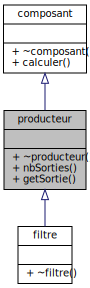
\includegraphics[width=350pt]{classproducteur__inherit__graph}
\end{center}
\end{figure}


Collaboration diagram for producteur\-:
\nopagebreak
\begin{figure}[H]
\begin{center}
\leavevmode
\includegraphics[width=144pt]{classproducteur__coll__graph}
\end{center}
\end{figure}
\subsection*{Public Member Functions}
\begin{DoxyCompactItemize}
\item 
virtual \hyperlink{classproducteur_a267b3a02f994c02436b300ea9a25a817}{$\sim$producteur} ()
\begin{DoxyCompactList}\small\item\em Destructeur virtuel. \end{DoxyCompactList}\item 
virtual unsigned int \hyperlink{classproducteur_abd95dacd17daa4479f213c7455ce0058}{nb\-Sorties} () const =0
\begin{DoxyCompactList}\small\item\em Nombre de sorties du composant. \end{DoxyCompactList}\item 
virtual const \hyperlink{classcounted__ptr}{counted\-\_\-ptr}$<$ \hyperlink{classflot}{flot} $>$ \& \hyperlink{classproducteur_a5673d0a0e8553ecf711e8338e4f6ab2e}{get\-Sortie} (unsigned int numsortie) const =0
\begin{DoxyCompactList}\small\item\em Recupération d'une sortie du composant. \end{DoxyCompactList}\end{DoxyCompactItemize}


\subsection{Detailed Description}
Interface d'un producteur d'échantillons sonores. Il s'agit d'une interface décrivant un composant ne possédant que des sorties. 

\begin{DoxyAuthor}{Author}
Jean Christophe Engel, Fabrice Lamarche, University Of Rennes 1 
\end{DoxyAuthor}
\begin{DoxyDate}{Date}
23/04/2010 
\end{DoxyDate}


\subsection{Constructor \& Destructor Documentation}
\hypertarget{classproducteur_a267b3a02f994c02436b300ea9a25a817}{\index{producteur@{producteur}!$\sim$producteur@{$\sim$producteur}}
\index{$\sim$producteur@{$\sim$producteur}!producteur@{producteur}}
\subsubsection[{$\sim$producteur}]{\setlength{\rightskip}{0pt plus 5cm}producteur\-::$\sim$producteur (
\begin{DoxyParamCaption}
{}
\end{DoxyParamCaption}
)\hspace{0.3cm}{\ttfamily [inline]}, {\ttfamily [virtual]}}}\label{classproducteur_a267b3a02f994c02436b300ea9a25a817}


Destructeur virtuel. 



\subsection{Member Function Documentation}
\hypertarget{classproducteur_a5673d0a0e8553ecf711e8338e4f6ab2e}{\index{producteur@{producteur}!get\-Sortie@{get\-Sortie}}
\index{get\-Sortie@{get\-Sortie}!producteur@{producteur}}
\subsubsection[{get\-Sortie}]{\setlength{\rightskip}{0pt plus 5cm}const {\bf counted\-\_\-ptr}$<$ {\bf flot} $>$ \& producteur\-::get\-Sortie (
\begin{DoxyParamCaption}
\item[{unsigned int}]{numsortie}
\end{DoxyParamCaption}
) const\hspace{0.3cm}{\ttfamily [pure virtual]}}}\label{classproducteur_a5673d0a0e8553ecf711e8338e4f6ab2e}


Recupération d'une sortie du composant. 


\begin{DoxyParams}{Parameters}
{\em numsortie} & Le numero de la sortie a recuperer. \\
\hline
\end{DoxyParams}
\begin{DoxyPrecond}{Precondition}
0 $<$= numsortie $<$ \hyperlink{classproducteur_abd95dacd17daa4479f213c7455ce0058}{nb\-Sorties()} 
\end{DoxyPrecond}
\begin{DoxyReturn}{Returns}
La sortie demandée. 
\end{DoxyReturn}


Implemented in \hyperlink{classproducteur__base_a96c01a2773c11eb0859150fc3a8e8338}{producteur\-\_\-base}.

\hypertarget{classproducteur_abd95dacd17daa4479f213c7455ce0058}{\index{producteur@{producteur}!nb\-Sorties@{nb\-Sorties}}
\index{nb\-Sorties@{nb\-Sorties}!producteur@{producteur}}
\subsubsection[{nb\-Sorties}]{\setlength{\rightskip}{0pt plus 5cm}unsigned int producteur\-::nb\-Sorties (
\begin{DoxyParamCaption}
{}
\end{DoxyParamCaption}
) const\hspace{0.3cm}{\ttfamily [pure virtual]}}}\label{classproducteur_abd95dacd17daa4479f213c7455ce0058}


Nombre de sorties du composant. 

\begin{DoxyReturn}{Returns}
Le nombre de sorties du composant. 
\end{DoxyReturn}


Implemented in \hyperlink{classproducteur__base_ae5148ef791b0f3c393e45e08e08c6246}{producteur\-\_\-base}.



The documentation for this class was generated from the following file\-:\begin{DoxyCompactItemize}
\item 
include/\hyperlink{producteur_8h}{producteur.\-h}\end{DoxyCompactItemize}

\hypertarget{classproducteur__base}{\section{producteur\-\_\-base Class Reference}
\label{classproducteur__base}\index{producteur\-\_\-base@{producteur\-\_\-base}}
}


{\ttfamily \#include $<$producteur\-\_\-base.\-h$>$}



Inheritance diagram for producteur\-\_\-base\-:
\nopagebreak
\begin{figure}[H]
\begin{center}
\leavevmode
\includegraphics[width=350pt]{classproducteur__base__inherit__graph}
\end{center}
\end{figure}


Collaboration diagram for producteur\-\_\-base\-:
\nopagebreak
\begin{figure}[H]
\begin{center}
\leavevmode
\includegraphics[width=168pt]{classproducteur__base__coll__graph}
\end{center}
\end{figure}
\subsection*{Public Member Functions}
\begin{DoxyCompactItemize}
\item 
\hyperlink{classproducteur__base_a0c2c488d98b77585e49b98d347910025}{producteur\-\_\-base} (unsigned int)
\item 
virtual \hyperlink{classproducteur__base_adc64c1151262d68209a09dea21c1ee58}{$\sim$producteur\-\_\-base} ()
\item 
virtual unsigned int \hyperlink{classproducteur__base_ae5148ef791b0f3c393e45e08e08c6246}{nb\-Sorties} () const 
\item 
virtual const \hyperlink{classcounted__ptr}{counted\-\_\-ptr}$<$ \hyperlink{classflot}{flot} $>$ \& \hyperlink{classproducteur__base_a96c01a2773c11eb0859150fc3a8e8338}{get\-Sortie} (unsigned int numsortie) const 
\item 
virtual void \hyperlink{classproducteur__base_af1e171c9e69b0998d5124c7389737f82}{calculer} ()=0
\begin{DoxyCompactList}\small\item\em Effectue les calculs associes au composant. \end{DoxyCompactList}\item 
virtual void \hyperlink{classproducteur__base_ad24519c3b05f7371ee15a9a402dc0717}{connecter\-Sortie} (const \hyperlink{classcounted__ptr}{counted\-\_\-ptr}$<$ \hyperlink{classflot}{flot} $>$ \&, unsigned int)
\end{DoxyCompactItemize}
\subsection*{Protected Attributes}
\begin{DoxyCompactItemize}
\item 
unsigned int \hyperlink{classproducteur__base_a6439bb4131b4644839f11849568d36fc}{m\-\_\-max\-\_\-output}
\item 
std\-::vector$<$ \hyperlink{classcounted__ptr}{counted\-\_\-ptr}$<$ \hyperlink{classflot}{flot} $>$ $>$ \hyperlink{classproducteur__base_abc5c0041e6ff23ce7a5c03ee7b9daf53}{m\-\_\-output}
\end{DoxyCompactItemize}


\subsection{Constructor \& Destructor Documentation}
\hypertarget{classproducteur__base_a0c2c488d98b77585e49b98d347910025}{\index{producteur\-\_\-base@{producteur\-\_\-base}!producteur\-\_\-base@{producteur\-\_\-base}}
\index{producteur\-\_\-base@{producteur\-\_\-base}!producteur_base@{producteur\-\_\-base}}
\subsubsection[{producteur\-\_\-base}]{\setlength{\rightskip}{0pt plus 5cm}producteur\-\_\-base\-::producteur\-\_\-base (
\begin{DoxyParamCaption}
\item[{unsigned int}]{outputs}
\end{DoxyParamCaption}
)}}\label{classproducteur__base_a0c2c488d98b77585e49b98d347910025}
Représente un producteur simple Possède outputs sorties \hypertarget{classproducteur__base_adc64c1151262d68209a09dea21c1ee58}{\index{producteur\-\_\-base@{producteur\-\_\-base}!$\sim$producteur\-\_\-base@{$\sim$producteur\-\_\-base}}
\index{$\sim$producteur\-\_\-base@{$\sim$producteur\-\_\-base}!producteur_base@{producteur\-\_\-base}}
\subsubsection[{$\sim$producteur\-\_\-base}]{\setlength{\rightskip}{0pt plus 5cm}virtual producteur\-\_\-base\-::$\sim$producteur\-\_\-base (
\begin{DoxyParamCaption}
{}
\end{DoxyParamCaption}
)\hspace{0.3cm}{\ttfamily [inline]}, {\ttfamily [virtual]}}}\label{classproducteur__base_adc64c1151262d68209a09dea21c1ee58}


\subsection{Member Function Documentation}
\hypertarget{classproducteur__base_af1e171c9e69b0998d5124c7389737f82}{\index{producteur\-\_\-base@{producteur\-\_\-base}!calculer@{calculer}}
\index{calculer@{calculer}!producteur_base@{producteur\-\_\-base}}
\subsubsection[{calculer}]{\setlength{\rightskip}{0pt plus 5cm}virtual void producteur\-\_\-base\-::calculer (
\begin{DoxyParamCaption}
{}
\end{DoxyParamCaption}
)\hspace{0.3cm}{\ttfamily [pure virtual]}}}\label{classproducteur__base_af1e171c9e69b0998d5124c7389737f82}


Effectue les calculs associes au composant. 



Implements \hyperlink{classcomposant_a257333d140850f51be479b025ce1e540}{composant}.



Implemented in \hyperlink{classoperation__binaire_a2ecfa3c6c05006c5c1bc285281bc6f3a}{operation\-\_\-binaire$<$ T $>$}, \hyperlink{classharmonique_a4dbd729dfa443204d9834effbb63d816}{harmonique}, \hyperlink{classfiltre__compose_a6fd1598c04300da43989af4f87a37aba}{filtre\-\_\-compose}, \hyperlink{classvolume_aab5a1f0490ea8b5826db6edd78e90f1d}{volume}, \hyperlink{classfile__reader_ac63890e9fbb85cda005efbce47f83648}{file\-\_\-reader}, \hyperlink{classsignal__constant_a18edd9db48afa7b287ae363bdcd91d43}{signal\-\_\-constant}, \hyperlink{classfiltre__base_ad06f5db1f851e5ad8655c9d8927cf347}{filtre\-\_\-base}, and \hyperlink{classmultiplicateur_ab22f15668247a10a35f027bd503f2442}{multiplicateur}.

\hypertarget{classproducteur__base_ad24519c3b05f7371ee15a9a402dc0717}{\index{producteur\-\_\-base@{producteur\-\_\-base}!connecter\-Sortie@{connecter\-Sortie}}
\index{connecter\-Sortie@{connecter\-Sortie}!producteur_base@{producteur\-\_\-base}}
\subsubsection[{connecter\-Sortie}]{\setlength{\rightskip}{0pt plus 5cm}void producteur\-\_\-base\-::connecter\-Sortie (
\begin{DoxyParamCaption}
\item[{const {\bf counted\-\_\-ptr}$<$ {\bf flot} $>$ \&}]{fl, }
\item[{unsigned int}]{nb\-Out}
\end{DoxyParamCaption}
)\hspace{0.3cm}{\ttfamily [virtual]}}}\label{classproducteur__base_ad24519c3b05f7371ee15a9a402dc0717}
Connecte le flot fl à la sortie nb\-Out \hypertarget{classproducteur__base_a96c01a2773c11eb0859150fc3a8e8338}{\index{producteur\-\_\-base@{producteur\-\_\-base}!get\-Sortie@{get\-Sortie}}
\index{get\-Sortie@{get\-Sortie}!producteur_base@{producteur\-\_\-base}}
\subsubsection[{get\-Sortie}]{\setlength{\rightskip}{0pt plus 5cm}const {\bf counted\-\_\-ptr}$<$ {\bf flot} $>$ \& producteur\-\_\-base\-::get\-Sortie (
\begin{DoxyParamCaption}
\item[{unsigned int}]{numsortie}
\end{DoxyParamCaption}
) const\hspace{0.3cm}{\ttfamily [virtual]}}}\label{classproducteur__base_a96c01a2773c11eb0859150fc3a8e8338}
Renvoie la sortie numsortie 

Implements \hyperlink{classproducteur_a5673d0a0e8553ecf711e8338e4f6ab2e}{producteur}.

\hypertarget{classproducteur__base_ae5148ef791b0f3c393e45e08e08c6246}{\index{producteur\-\_\-base@{producteur\-\_\-base}!nb\-Sorties@{nb\-Sorties}}
\index{nb\-Sorties@{nb\-Sorties}!producteur_base@{producteur\-\_\-base}}
\subsubsection[{nb\-Sorties}]{\setlength{\rightskip}{0pt plus 5cm}unsigned int producteur\-\_\-base\-::nb\-Sorties (
\begin{DoxyParamCaption}
{}
\end{DoxyParamCaption}
) const\hspace{0.3cm}{\ttfamily [virtual]}}}\label{classproducteur__base_ae5148ef791b0f3c393e45e08e08c6246}
Renvoie le nombre de sorties de ce producteur 

Implements \hyperlink{classproducteur_abd95dacd17daa4479f213c7455ce0058}{producteur}.



\subsection{Member Data Documentation}
\hypertarget{classproducteur__base_a6439bb4131b4644839f11849568d36fc}{\index{producteur\-\_\-base@{producteur\-\_\-base}!m\-\_\-max\-\_\-output@{m\-\_\-max\-\_\-output}}
\index{m\-\_\-max\-\_\-output@{m\-\_\-max\-\_\-output}!producteur_base@{producteur\-\_\-base}}
\subsubsection[{m\-\_\-max\-\_\-output}]{\setlength{\rightskip}{0pt plus 5cm}unsigned int producteur\-\_\-base\-::m\-\_\-max\-\_\-output\hspace{0.3cm}{\ttfamily [protected]}}}\label{classproducteur__base_a6439bb4131b4644839f11849568d36fc}
Nombre maximal de sorties \hypertarget{classproducteur__base_abc5c0041e6ff23ce7a5c03ee7b9daf53}{\index{producteur\-\_\-base@{producteur\-\_\-base}!m\-\_\-output@{m\-\_\-output}}
\index{m\-\_\-output@{m\-\_\-output}!producteur_base@{producteur\-\_\-base}}
\subsubsection[{m\-\_\-output}]{\setlength{\rightskip}{0pt plus 5cm}std\-::vector$<${\bf counted\-\_\-ptr}$<${\bf flot}$>$ $>$ producteur\-\_\-base\-::m\-\_\-output\hspace{0.3cm}{\ttfamily [protected]}}}\label{classproducteur__base_abc5c0041e6ff23ce7a5c03ee7b9daf53}
Liste des sorties 

The documentation for this class was generated from the following files\-:\begin{DoxyCompactItemize}
\item 
src/\hyperlink{producteur__base_8h}{producteur\-\_\-base.\-h}\item 
src/\hyperlink{producteur__base_8cpp}{producteur\-\_\-base.\-cpp}\end{DoxyCompactItemize}

\hypertarget{classsignal__constant}{\section{signal\-\_\-constant Class Reference}
\label{classsignal__constant}\index{signal\-\_\-constant@{signal\-\_\-constant}}
}


{\ttfamily \#include $<$signal\-\_\-constant.\-h$>$}



Inheritance diagram for signal\-\_\-constant\-:
\nopagebreak
\begin{figure}[H]
\begin{center}
\leavevmode
\includegraphics[width=168pt]{classsignal__constant__inherit__graph}
\end{center}
\end{figure}


Collaboration diagram for signal\-\_\-constant\-:
\nopagebreak
\begin{figure}[H]
\begin{center}
\leavevmode
\includegraphics[width=168pt]{classsignal__constant__coll__graph}
\end{center}
\end{figure}
\subsection*{Public Member Functions}
\begin{DoxyCompactItemize}
\item 
\hyperlink{classsignal__constant_a49639918bd5ecb949829f34703b21044}{signal\-\_\-constant} (double)
\item 
virtual \hyperlink{classsignal__constant_aa4c913cb08d9be90799b5f30fbb208fa}{$\sim$signal\-\_\-constant} ()
\item 
virtual void \hyperlink{classsignal__constant_a18edd9db48afa7b287ae363bdcd91d43}{calculer} ()
\end{DoxyCompactItemize}
\subsection*{Private Attributes}
\begin{DoxyCompactItemize}
\item 
double \hyperlink{classsignal__constant_a750ff715be3882c6838312ffddf025b8}{m\-\_\-val}
\end{DoxyCompactItemize}
\subsection*{Additional Inherited Members}


\subsection{Constructor \& Destructor Documentation}
\hypertarget{classsignal__constant_a49639918bd5ecb949829f34703b21044}{\index{signal\-\_\-constant@{signal\-\_\-constant}!signal\-\_\-constant@{signal\-\_\-constant}}
\index{signal\-\_\-constant@{signal\-\_\-constant}!signal_constant@{signal\-\_\-constant}}
\subsubsection[{signal\-\_\-constant}]{\setlength{\rightskip}{0pt plus 5cm}signal\-\_\-constant\-::signal\-\_\-constant (
\begin{DoxyParamCaption}
\item[{double}]{val}
\end{DoxyParamCaption}
)}}\label{classsignal__constant_a49639918bd5ecb949829f34703b21044}
Représente un signal constant (compris entre -\/1 et 1) \hypertarget{classsignal__constant_aa4c913cb08d9be90799b5f30fbb208fa}{\index{signal\-\_\-constant@{signal\-\_\-constant}!$\sim$signal\-\_\-constant@{$\sim$signal\-\_\-constant}}
\index{$\sim$signal\-\_\-constant@{$\sim$signal\-\_\-constant}!signal_constant@{signal\-\_\-constant}}
\subsubsection[{$\sim$signal\-\_\-constant}]{\setlength{\rightskip}{0pt plus 5cm}virtual signal\-\_\-constant\-::$\sim$signal\-\_\-constant (
\begin{DoxyParamCaption}
{}
\end{DoxyParamCaption}
)\hspace{0.3cm}{\ttfamily [inline]}, {\ttfamily [virtual]}}}\label{classsignal__constant_aa4c913cb08d9be90799b5f30fbb208fa}


\subsection{Member Function Documentation}
\hypertarget{classsignal__constant_a18edd9db48afa7b287ae363bdcd91d43}{\index{signal\-\_\-constant@{signal\-\_\-constant}!calculer@{calculer}}
\index{calculer@{calculer}!signal_constant@{signal\-\_\-constant}}
\subsubsection[{calculer}]{\setlength{\rightskip}{0pt plus 5cm}void signal\-\_\-constant\-::calculer (
\begin{DoxyParamCaption}
{}
\end{DoxyParamCaption}
)\hspace{0.3cm}{\ttfamily [virtual]}}}\label{classsignal__constant_a18edd9db48afa7b287ae363bdcd91d43}
Calcule la prochaine valeur (toujours la même) 

Implements \hyperlink{classproducteur__base_af1e171c9e69b0998d5124c7389737f82}{producteur\-\_\-base}.



\subsection{Member Data Documentation}
\hypertarget{classsignal__constant_a750ff715be3882c6838312ffddf025b8}{\index{signal\-\_\-constant@{signal\-\_\-constant}!m\-\_\-val@{m\-\_\-val}}
\index{m\-\_\-val@{m\-\_\-val}!signal_constant@{signal\-\_\-constant}}
\subsubsection[{m\-\_\-val}]{\setlength{\rightskip}{0pt plus 5cm}double signal\-\_\-constant\-::m\-\_\-val\hspace{0.3cm}{\ttfamily [private]}}}\label{classsignal__constant_a750ff715be3882c6838312ffddf025b8}
Valeur à renvoyer à chaque fois. 

The documentation for this class was generated from the following files\-:\begin{DoxyCompactItemize}
\item 
src/\hyperlink{signal__constant_8h}{signal\-\_\-constant.\-h}\item 
src/\hyperlink{signal__constant_8cpp}{signal\-\_\-constant.\-cpp}\end{DoxyCompactItemize}

\hypertarget{classvolume}{\section{volume Class Reference}
\label{classvolume}\index{volume@{volume}}
}


{\ttfamily \#include $<$volume.\-h$>$}



Inheritance diagram for volume\-:
\nopagebreak
\begin{figure}[H]
\begin{center}
\leavevmode
\includegraphics[width=346pt]{classvolume__inherit__graph}
\end{center}
\end{figure}


Collaboration diagram for volume\-:
\nopagebreak
\begin{figure}[H]
\begin{center}
\leavevmode
\includegraphics[width=346pt]{classvolume__coll__graph}
\end{center}
\end{figure}
\subsection*{Public Member Functions}
\begin{DoxyCompactItemize}
\item 
\hyperlink{classvolume_a94d2ba725bfa08519d625e0bee5445d9}{volume} (double)
\item 
virtual \hyperlink{classvolume_ae5872ddf030fb8f9667f3443937cfd2f}{$\sim$volume} ()
\item 
virtual void \hyperlink{classvolume_aab5a1f0490ea8b5826db6edd78e90f1d}{calculer} ()
\item 
virtual void \hyperlink{classvolume_a5ee6dc194dc9d47c9d554a4f94ac0512}{connecter\-Entree} (const \hyperlink{classcounted__ptr}{counted\-\_\-ptr}$<$ \hyperlink{classflot}{flot} $>$ \&, unsigned int)
\end{DoxyCompactItemize}
\subsection*{Private Attributes}
\begin{DoxyCompactItemize}
\item 
\hyperlink{classmultiplicateur}{multiplicateur} \hyperlink{classvolume_a882a7cff6324a567d4295239811be846}{m\-\_\-mul}
\item 
\hyperlink{classsignal__constant}{signal\-\_\-constant} \hyperlink{classvolume_af992e96f1c1aedd23a4a9ef5f13eb726}{m\-\_\-vol}
\end{DoxyCompactItemize}
\subsection*{Additional Inherited Members}


\subsection{Constructor \& Destructor Documentation}
\hypertarget{classvolume_a94d2ba725bfa08519d625e0bee5445d9}{\index{volume@{volume}!volume@{volume}}
\index{volume@{volume}!volume@{volume}}
\subsubsection[{volume}]{\setlength{\rightskip}{0pt plus 5cm}volume\-::volume (
\begin{DoxyParamCaption}
\item[{double}]{factor}
\end{DoxyParamCaption}
)}}\label{classvolume_a94d2ba725bfa08519d625e0bee5445d9}
Permet de modifier le volume en le multipliant avec un signal constant \hypertarget{classvolume_ae5872ddf030fb8f9667f3443937cfd2f}{\index{volume@{volume}!$\sim$volume@{$\sim$volume}}
\index{$\sim$volume@{$\sim$volume}!volume@{volume}}
\subsubsection[{$\sim$volume}]{\setlength{\rightskip}{0pt plus 5cm}virtual volume\-::$\sim$volume (
\begin{DoxyParamCaption}
{}
\end{DoxyParamCaption}
)\hspace{0.3cm}{\ttfamily [inline]}, {\ttfamily [virtual]}}}\label{classvolume_ae5872ddf030fb8f9667f3443937cfd2f}


\subsection{Member Function Documentation}
\hypertarget{classvolume_aab5a1f0490ea8b5826db6edd78e90f1d}{\index{volume@{volume}!calculer@{calculer}}
\index{calculer@{calculer}!volume@{volume}}
\subsubsection[{calculer}]{\setlength{\rightskip}{0pt plus 5cm}void volume\-::calculer (
\begin{DoxyParamCaption}
{}
\end{DoxyParamCaption}
)\hspace{0.3cm}{\ttfamily [virtual]}}}\label{classvolume_aab5a1f0490ea8b5826db6edd78e90f1d}
Calcule la prochaine valeur (volume diminué) 

Implements \hyperlink{classfiltre__base_ad06f5db1f851e5ad8655c9d8927cf347}{filtre\-\_\-base}.

\hypertarget{classvolume_a5ee6dc194dc9d47c9d554a4f94ac0512}{\index{volume@{volume}!connecter\-Entree@{connecter\-Entree}}
\index{connecter\-Entree@{connecter\-Entree}!volume@{volume}}
\subsubsection[{connecter\-Entree}]{\setlength{\rightskip}{0pt plus 5cm}void volume\-::connecter\-Entree (
\begin{DoxyParamCaption}
\item[{const {\bf counted\-\_\-ptr}$<$ {\bf flot} $>$ \&}]{fl, }
\item[{unsigned int}]{in}
\end{DoxyParamCaption}
)\hspace{0.3cm}{\ttfamily [virtual]}}}\label{classvolume_a5ee6dc194dc9d47c9d554a4f94ac0512}
Connecte une entrée au composant en lui appliquant le volume 

Reimplemented from \hyperlink{classconsommateur__base_a273d1899ba7e05e8651b4cca6aa35b1d}{consommateur\-\_\-base}.



\subsection{Member Data Documentation}
\hypertarget{classvolume_a882a7cff6324a567d4295239811be846}{\index{volume@{volume}!m\-\_\-mul@{m\-\_\-mul}}
\index{m\-\_\-mul@{m\-\_\-mul}!volume@{volume}}
\subsubsection[{m\-\_\-mul}]{\setlength{\rightskip}{0pt plus 5cm}{\bf multiplicateur} volume\-::m\-\_\-mul\hspace{0.3cm}{\ttfamily [private]}}}\label{classvolume_a882a7cff6324a567d4295239811be846}
Multiplicateur permettant d'appliquer le volume \hypertarget{classvolume_af992e96f1c1aedd23a4a9ef5f13eb726}{\index{volume@{volume}!m\-\_\-vol@{m\-\_\-vol}}
\index{m\-\_\-vol@{m\-\_\-vol}!volume@{volume}}
\subsubsection[{m\-\_\-vol}]{\setlength{\rightskip}{0pt plus 5cm}{\bf signal\-\_\-constant} volume\-::m\-\_\-vol\hspace{0.3cm}{\ttfamily [private]}}}\label{classvolume_af992e96f1c1aedd23a4a9ef5f13eb726}
Facteur de volume (uniquement descendant) 

The documentation for this class was generated from the following files\-:\begin{DoxyCompactItemize}
\item 
src/\hyperlink{volume_8h}{volume.\-h}\item 
src/\hyperlink{volume_8cpp}{volume.\-cpp}\end{DoxyCompactItemize}

\hypertarget{classvolume__compose}{\section{volume\-\_\-compose Class Reference}
\label{classvolume__compose}\index{volume\-\_\-compose@{volume\-\_\-compose}}
}


{\ttfamily \#include $<$volume\-\_\-compose.\-h$>$}



Inheritance diagram for volume\-\_\-compose\-:
\nopagebreak
\begin{figure}[H]
\begin{center}
\leavevmode
\includegraphics[width=346pt]{classvolume__compose__inherit__graph}
\end{center}
\end{figure}


Collaboration diagram for volume\-\_\-compose\-:
\nopagebreak
\begin{figure}[H]
\begin{center}
\leavevmode
\includegraphics[width=346pt]{classvolume__compose__coll__graph}
\end{center}
\end{figure}
\subsection*{Public Member Functions}
\begin{DoxyCompactItemize}
\item 
\hyperlink{classvolume__compose_a3ac65c841ee3c62547ff06fc8d0d6189}{volume\-\_\-compose} (double)
\item 
virtual \hyperlink{classvolume__compose_a9d46c6f3b0ca645fc57c04fdc40fc5d7}{$\sim$volume\-\_\-compose} ()
\end{DoxyCompactItemize}
\subsection*{Additional Inherited Members}


\subsection{Constructor \& Destructor Documentation}
\hypertarget{classvolume__compose_a3ac65c841ee3c62547ff06fc8d0d6189}{\index{volume\-\_\-compose@{volume\-\_\-compose}!volume\-\_\-compose@{volume\-\_\-compose}}
\index{volume\-\_\-compose@{volume\-\_\-compose}!volume_compose@{volume\-\_\-compose}}
\subsubsection[{volume\-\_\-compose}]{\setlength{\rightskip}{0pt plus 5cm}volume\-\_\-compose\-::volume\-\_\-compose (
\begin{DoxyParamCaption}
\item[{double}]{vol}
\end{DoxyParamCaption}
)}}\label{classvolume__compose_a3ac65c841ee3c62547ff06fc8d0d6189}
Répresente un facteur de volume construit à partir d'un filtre composé N\-O\-T\-E\-: vol = 0.\-5 \-: -\/3d\-B \hypertarget{classvolume__compose_a9d46c6f3b0ca645fc57c04fdc40fc5d7}{\index{volume\-\_\-compose@{volume\-\_\-compose}!$\sim$volume\-\_\-compose@{$\sim$volume\-\_\-compose}}
\index{$\sim$volume\-\_\-compose@{$\sim$volume\-\_\-compose}!volume_compose@{volume\-\_\-compose}}
\subsubsection[{$\sim$volume\-\_\-compose}]{\setlength{\rightskip}{0pt plus 5cm}virtual volume\-\_\-compose\-::$\sim$volume\-\_\-compose (
\begin{DoxyParamCaption}
{}
\end{DoxyParamCaption}
)\hspace{0.3cm}{\ttfamily [inline]}, {\ttfamily [virtual]}}}\label{classvolume__compose_a9d46c6f3b0ca645fc57c04fdc40fc5d7}


The documentation for this class was generated from the following files\-:\begin{DoxyCompactItemize}
\item 
src/\hyperlink{volume__compose_8h}{volume\-\_\-compose.\-h}\item 
src/\hyperlink{volume__compose_8cpp}{volume\-\_\-compose.\-cpp}\end{DoxyCompactItemize}

\chapter{File Documentation}
\hypertarget{composant_8h}{\section{include/composant.h File Reference}
\label{composant_8h}\index{include/composant.\-h@{include/composant.\-h}}
}
This graph shows which files directly or indirectly include this file\-:
\nopagebreak
\begin{figure}[H]
\begin{center}
\leavevmode
\includegraphics[width=350pt]{composant_8h__dep__incl}
\end{center}
\end{figure}
\subsection*{Classes}
\begin{DoxyCompactItemize}
\item 
class \hyperlink{classcomposant}{composant}
\begin{DoxyCompactList}\small\item\em Interface d'un composant du systeme sonore. \end{DoxyCompactList}\end{DoxyCompactItemize}

\hypertarget{composant__exception_8h}{\section{include/composant\-\_\-exception.h File Reference}
\label{composant__exception_8h}\index{include/composant\-\_\-exception.\-h@{include/composant\-\_\-exception.\-h}}
}
{\ttfamily \#include $<$exception$>$}\\*
{\ttfamily \#include $<$string$>$}\\*
Include dependency graph for composant\-\_\-exception.\-h\-:
\nopagebreak
\begin{figure}[H]
\begin{center}
\leavevmode
\includegraphics[width=234pt]{composant__exception_8h__incl}
\end{center}
\end{figure}
This graph shows which files directly or indirectly include this file\-:
\nopagebreak
\begin{figure}[H]
\begin{center}
\leavevmode
\includegraphics[width=234pt]{composant__exception_8h__dep__incl}
\end{center}
\end{figure}
\subsection*{Classes}
\begin{DoxyCompactItemize}
\item 
class \hyperlink{classcomposant__exception}{composant\-\_\-exception}
\begin{DoxyCompactList}\small\item\em classe qui gère les exceptions liées à un composant \end{DoxyCompactList}\end{DoxyCompactItemize}

\hypertarget{consommateur_8h}{\section{include/consommateur.h File Reference}
\label{consommateur_8h}\index{include/consommateur.\-h@{include/consommateur.\-h}}
}
{\ttfamily \#include \char`\"{}composant.\-h\char`\"{}}\\*
{\ttfamily \#include \char`\"{}flot.\-h\char`\"{}}\\*
{\ttfamily \#include \char`\"{}counted\-\_\-ptr.\-h\char`\"{}}\\*
Include dependency graph for consommateur.\-h\-:
\nopagebreak
\begin{figure}[H]
\begin{center}
\leavevmode
\includegraphics[width=302pt]{consommateur_8h__incl}
\end{center}
\end{figure}
This graph shows which files directly or indirectly include this file\-:
\nopagebreak
\begin{figure}[H]
\begin{center}
\leavevmode
\includegraphics[width=350pt]{consommateur_8h__dep__incl}
\end{center}
\end{figure}
\subsection*{Classes}
\begin{DoxyCompactItemize}
\item 
class \hyperlink{classconsommateur}{consommateur}
\begin{DoxyCompactList}\small\item\em Interface d'un consommateur d'échantillons sonores. Il s'agit d'une interface décrivant un composant qui ne possède que des entrées. \end{DoxyCompactList}\end{DoxyCompactItemize}

\hypertarget{constantes_8h}{\section{include/constantes.h File Reference}
\label{constantes_8h}\index{include/constantes.\-h@{include/constantes.\-h}}
}
This graph shows which files directly or indirectly include this file\-:
\nopagebreak
\begin{figure}[H]
\begin{center}
\leavevmode
\includegraphics[width=350pt]{constantes_8h__dep__incl}
\end{center}
\end{figure}
\subsection*{Namespaces}
\begin{DoxyCompactItemize}
\item 
\hyperlink{namespaceMixageSonore}{Mixage\-Sonore}
\end{DoxyCompactItemize}
\subsection*{Variables}
\begin{DoxyCompactItemize}
\item 
static const double \hyperlink{namespaceMixageSonore_a74eacef80ae62303d777e9b6791cd8af}{Mixage\-Sonore\-::pi} = 3.\-14159265358979323846
\begin{DoxyCompactList}\small\item\em Constante définissant la valeur de P\-I. \end{DoxyCompactList}\item 
static const unsigned int \hyperlink{namespaceMixageSonore_a9625ad51e0845108a6c3ef4ec340adc6}{Mixage\-Sonore\-::frequency} = 44100
\begin{DoxyCompactList}\small\item\em Constante représentant la fréquence d'échantillonnage des samples sonores. \end{DoxyCompactList}\item 
static const unsigned int \hyperlink{namespaceMixageSonore_a1d6118bf5d0d09e5be4136d50f2ac887}{Mixage\-Sonore\-::taille\-Echantillon} = 2
\begin{DoxyCompactList}\small\item\em taille en octets d'un échantillon (entrées/sorties fichier) \end{DoxyCompactList}\end{DoxyCompactItemize}

\hypertarget{counted__ptr_8h}{\section{include/counted\-\_\-ptr.h File Reference}
\label{counted__ptr_8h}\index{include/counted\-\_\-ptr.\-h@{include/counted\-\_\-ptr.\-h}}
}
{\ttfamily \#include $<$cassert$>$}\\*
Include dependency graph for counted\-\_\-ptr.\-h\-:
\nopagebreak
\begin{figure}[H]
\begin{center}
\leavevmode
\includegraphics[width=188pt]{counted__ptr_8h__incl}
\end{center}
\end{figure}
This graph shows which files directly or indirectly include this file\-:
\nopagebreak
\begin{figure}[H]
\begin{center}
\leavevmode
\includegraphics[width=350pt]{counted__ptr_8h__dep__incl}
\end{center}
\end{figure}
\subsection*{Classes}
\begin{DoxyCompactItemize}
\item 
class \hyperlink{classcounted__ptr}{counted\-\_\-ptr$<$ T $>$}
\begin{DoxyCompactList}\small\item\em Classe gérant un \char`\"{}smart pointer\char`\"{}. \end{DoxyCompactList}\end{DoxyCompactItemize}

\hypertarget{enregistreur__fichier_8h}{\section{include/enregistreur\-\_\-fichier.h File Reference}
\label{enregistreur__fichier_8h}\index{include/enregistreur\-\_\-fichier.\-h@{include/enregistreur\-\_\-fichier.\-h}}
}
{\ttfamily \#include $<$fstream$>$}\\*
{\ttfamily \#include $<$vector$>$}\\*
{\ttfamily \#include \char`\"{}consommateur.\-h\char`\"{}}\\*
{\ttfamily \#include \char`\"{}constantes.\-h\char`\"{}}\\*
Include dependency graph for enregistreur\-\_\-fichier.\-h\-:
\nopagebreak
\begin{figure}[H]
\begin{center}
\leavevmode
\includegraphics[width=350pt]{enregistreur__fichier_8h__incl}
\end{center}
\end{figure}
This graph shows which files directly or indirectly include this file\-:
\nopagebreak
\begin{figure}[H]
\begin{center}
\leavevmode
\includegraphics[width=180pt]{enregistreur__fichier_8h__dep__incl}
\end{center}
\end{figure}
\subsection*{Classes}
\begin{DoxyCompactItemize}
\item 
class \hyperlink{classenregistreur__fichier}{enregistreur\-\_\-fichier}
\begin{DoxyCompactList}\small\item\em Un consommateur qui enregistre ses entrées dans un fichier binaire ; 44100 Hz, 16bits signé, entrelacé \end{DoxyCompactList}\end{DoxyCompactItemize}

\hypertarget{enregistreur__fichier__texte_8h}{\section{include/enregistreur\-\_\-fichier\-\_\-texte.h File Reference}
\label{enregistreur__fichier__texte_8h}\index{include/enregistreur\-\_\-fichier\-\_\-texte.\-h@{include/enregistreur\-\_\-fichier\-\_\-texte.\-h}}
}
{\ttfamily \#include $<$fstream$>$}\\*
{\ttfamily \#include $<$vector$>$}\\*
{\ttfamily \#include \char`\"{}consommateur.\-h\char`\"{}}\\*
{\ttfamily \#include \char`\"{}constantes.\-h\char`\"{}}\\*
Include dependency graph for enregistreur\-\_\-fichier\-\_\-texte.\-h\-:
\nopagebreak
\begin{figure}[H]
\begin{center}
\leavevmode
\includegraphics[width=350pt]{enregistreur__fichier__texte_8h__incl}
\end{center}
\end{figure}
This graph shows which files directly or indirectly include this file\-:
\nopagebreak
\begin{figure}[H]
\begin{center}
\leavevmode
\includegraphics[width=180pt]{enregistreur__fichier__texte_8h__dep__incl}
\end{center}
\end{figure}
\subsection*{Classes}
\begin{DoxyCompactItemize}
\item 
class \hyperlink{classenregistreur__fichier__texte}{enregistreur\-\_\-fichier\-\_\-texte}
\begin{DoxyCompactList}\small\item\em Un consommateur qui enregistre ses entrées dans un fichier texte ; une ligne = un échantillon de chaque canal. \end{DoxyCompactList}\end{DoxyCompactItemize}

\hypertarget{filtre_8h}{\section{include/filtre.h File Reference}
\label{filtre_8h}\index{include/filtre.\-h@{include/filtre.\-h}}
}
{\ttfamily \#include \char`\"{}producteur.\-h\char`\"{}}\\*
{\ttfamily \#include \char`\"{}consommateur.\-h\char`\"{}}\\*
Include dependency graph for filtre.\-h\-:
\nopagebreak
\begin{figure}[H]
\begin{center}
\leavevmode
\includegraphics[width=302pt]{filtre_8h__incl}
\end{center}
\end{figure}
This graph shows which files directly or indirectly include this file\-:
\nopagebreak
\begin{figure}[H]
\begin{center}
\leavevmode
\includegraphics[width=350pt]{filtre_8h__dep__incl}
\end{center}
\end{figure}
\subsection*{Classes}
\begin{DoxyCompactItemize}
\item 
class \hyperlink{classfiltre}{filtre}
\begin{DoxyCompactList}\small\item\em Interface associée à un filtre sonore. Ce filtre est considéré comme un producteur / consommateur d'échantillons sonores. Il possède donc des entrées et des sorties. \end{DoxyCompactList}\end{DoxyCompactItemize}

\hypertarget{flot_8h}{\section{include/flot.h File Reference}
\label{flot_8h}\index{include/flot.\-h@{include/flot.\-h}}
}
This graph shows which files directly or indirectly include this file\-:
\nopagebreak
\begin{figure}[H]
\begin{center}
\leavevmode
\includegraphics[width=350pt]{flot_8h__dep__incl}
\end{center}
\end{figure}
\subsection*{Classes}
\begin{DoxyCompactItemize}
\item 
class \hyperlink{classflot}{flot}
\begin{DoxyCompactList}\small\item\em Interface associee a un flot de donnees reliant deux composants du systeme. \end{DoxyCompactList}\end{DoxyCompactItemize}

\hypertarget{producteur_8h}{\section{include/producteur.h File Reference}
\label{producteur_8h}\index{include/producteur.\-h@{include/producteur.\-h}}
}
{\ttfamily \#include \char`\"{}composant.\-h\char`\"{}}\\*
{\ttfamily \#include \char`\"{}flot.\-h\char`\"{}}\\*
{\ttfamily \#include \char`\"{}counted\-\_\-ptr.\-h\char`\"{}}\\*
Include dependency graph for producteur.\-h\-:
\nopagebreak
\begin{figure}[H]
\begin{center}
\leavevmode
\includegraphics[width=302pt]{producteur_8h__incl}
\end{center}
\end{figure}
This graph shows which files directly or indirectly include this file\-:
\nopagebreak
\begin{figure}[H]
\begin{center}
\leavevmode
\includegraphics[width=350pt]{producteur_8h__dep__incl}
\end{center}
\end{figure}
\subsection*{Classes}
\begin{DoxyCompactItemize}
\item 
class \hyperlink{classproducteur}{producteur}
\begin{DoxyCompactList}\small\item\em Interface d'un producteur d'échantillons sonores. Il s'agit d'une interface décrivant un composant ne possédant que des sorties. \end{DoxyCompactList}\end{DoxyCompactItemize}

\hypertarget{consommateur__base_8cpp}{\section{src/consommateur\-\_\-base.cpp File Reference}
\label{consommateur__base_8cpp}\index{src/consommateur\-\_\-base.\-cpp@{src/consommateur\-\_\-base.\-cpp}}
}
{\ttfamily \#include \char`\"{}consommateur\-\_\-base.\-h\char`\"{}}\\*
{\ttfamily \#include \char`\"{}imp\-\_\-flot.\-h\char`\"{}}\\*
Include dependency graph for consommateur\-\_\-base.\-cpp\-:
\nopagebreak
\begin{figure}[H]
\begin{center}
\leavevmode
\includegraphics[width=350pt]{consommateur__base_8cpp__incl}
\end{center}
\end{figure}

\hypertarget{consommateur__base_8h}{\section{src/consommateur\-\_\-base.h File Reference}
\label{consommateur__base_8h}\index{src/consommateur\-\_\-base.\-h@{src/consommateur\-\_\-base.\-h}}
}
{\ttfamily \#include \char`\"{}consommateur.\-h\char`\"{}}\\*
{\ttfamily \#include \char`\"{}counted\-\_\-ptr.\-h\char`\"{}}\\*
{\ttfamily \#include \char`\"{}flot.\-h\char`\"{}}\\*
{\ttfamily \#include $<$vector$>$}\\*
Include dependency graph for consommateur\-\_\-base.\-h\-:
\nopagebreak
\begin{figure}[H]
\begin{center}
\leavevmode
\includegraphics[width=318pt]{consommateur__base_8h__incl}
\end{center}
\end{figure}
This graph shows which files directly or indirectly include this file\-:
\nopagebreak
\begin{figure}[H]
\begin{center}
\leavevmode
\includegraphics[width=350pt]{consommateur__base_8h__dep__incl}
\end{center}
\end{figure}
\subsection*{Classes}
\begin{DoxyCompactItemize}
\item 
class \hyperlink{classconsommateur__base}{consommateur\-\_\-base}
\end{DoxyCompactItemize}

\hypertarget{file__reader_8cpp}{\section{src/file\-\_\-reader.cpp File Reference}
\label{file__reader_8cpp}\index{src/file\-\_\-reader.\-cpp@{src/file\-\_\-reader.\-cpp}}
}
{\ttfamily \#include \char`\"{}file\-\_\-reader.\-h\char`\"{}}\\*
{\ttfamily \#include \char`\"{}composant\-\_\-exception.\-h\char`\"{}}\\*
{\ttfamily \#include $<$climits$>$}\\*
Include dependency graph for file\-\_\-reader.\-cpp\-:
\nopagebreak
\begin{figure}[H]
\begin{center}
\leavevmode
\includegraphics[width=350pt]{file__reader_8cpp__incl}
\end{center}
\end{figure}

\hypertarget{file__reader_8h}{\section{src/file\-\_\-reader.h File Reference}
\label{file__reader_8h}\index{src/file\-\_\-reader.\-h@{src/file\-\_\-reader.\-h}}
}
{\ttfamily \#include \char`\"{}producteur\-\_\-base.\-h\char`\"{}}\\*
{\ttfamily \#include $<$fstream$>$}\\*
Include dependency graph for file\-\_\-reader.\-h\-:
\nopagebreak
\begin{figure}[H]
\begin{center}
\leavevmode
\includegraphics[width=321pt]{file__reader_8h__incl}
\end{center}
\end{figure}
This graph shows which files directly or indirectly include this file\-:
\nopagebreak
\begin{figure}[H]
\begin{center}
\leavevmode
\includegraphics[width=267pt]{file__reader_8h__dep__incl}
\end{center}
\end{figure}
\subsection*{Classes}
\begin{DoxyCompactItemize}
\item 
class \hyperlink{classfile__reader}{file\-\_\-reader}
\end{DoxyCompactItemize}

\hypertarget{filtre__base_8cpp}{\section{src/filtre\-\_\-base.cpp File Reference}
\label{filtre__base_8cpp}\index{src/filtre\-\_\-base.\-cpp@{src/filtre\-\_\-base.\-cpp}}
}
{\ttfamily \#include \char`\"{}filtre\-\_\-base.\-h\char`\"{}}\\*
Include dependency graph for filtre\-\_\-base.\-cpp\-:
\nopagebreak
\begin{figure}[H]
\begin{center}
\leavevmode
\includegraphics[width=350pt]{filtre__base_8cpp__incl}
\end{center}
\end{figure}

\hypertarget{filtre__base_8h}{\section{src/filtre\-\_\-base.h File Reference}
\label{filtre__base_8h}\index{src/filtre\-\_\-base.\-h@{src/filtre\-\_\-base.\-h}}
}
{\ttfamily \#include \char`\"{}filtre.\-h\char`\"{}}\\*
{\ttfamily \#include \char`\"{}counted\-\_\-ptr.\-h\char`\"{}}\\*
{\ttfamily \#include \char`\"{}producteur\-\_\-base.\-h\char`\"{}}\\*
{\ttfamily \#include \char`\"{}consommateur\-\_\-base.\-h\char`\"{}}\\*
Include dependency graph for filtre\-\_\-base.\-h\-:
\nopagebreak
\begin{figure}[H]
\begin{center}
\leavevmode
\includegraphics[width=350pt]{filtre__base_8h__incl}
\end{center}
\end{figure}
This graph shows which files directly or indirectly include this file\-:
\nopagebreak
\begin{figure}[H]
\begin{center}
\leavevmode
\includegraphics[width=350pt]{filtre__base_8h__dep__incl}
\end{center}
\end{figure}
\subsection*{Classes}
\begin{DoxyCompactItemize}
\item 
class \hyperlink{classfiltre__base}{filtre\-\_\-base}
\end{DoxyCompactItemize}

\hypertarget{filtre__compose_8cpp}{\section{src/filtre\-\_\-compose.cpp File Reference}
\label{filtre__compose_8cpp}\index{src/filtre\-\_\-compose.\-cpp@{src/filtre\-\_\-compose.\-cpp}}
}
{\ttfamily \#include \char`\"{}filtre\-\_\-compose.\-h\char`\"{}}\\*
{\ttfamily \#include $<$iostream$>$}\\*
{\ttfamily \#include $<$cstdlib$>$}\\*
Include dependency graph for filtre\-\_\-compose.\-cpp\-:
\nopagebreak
\begin{figure}[H]
\begin{center}
\leavevmode
\includegraphics[width=350pt]{filtre__compose_8cpp__incl}
\end{center}
\end{figure}

\hypertarget{filtre__compose_8h}{\section{src/filtre\-\_\-compose.h File Reference}
\label{filtre__compose_8h}\index{src/filtre\-\_\-compose.\-h@{src/filtre\-\_\-compose.\-h}}
}
{\ttfamily \#include \char`\"{}filtre\-\_\-base.\-h\char`\"{}}\\*
{\ttfamily \#include \char`\"{}composant.\-h\char`\"{}}\\*
{\ttfamily \#include $<$vector$>$}\\*
{\ttfamily \#include $<$map$>$}\\*
Include dependency graph for filtre\-\_\-compose.\-h\-:
\nopagebreak
\begin{figure}[H]
\begin{center}
\leavevmode
\includegraphics[width=350pt]{filtre__compose_8h__incl}
\end{center}
\end{figure}
This graph shows which files directly or indirectly include this file\-:
\nopagebreak
\begin{figure}[H]
\begin{center}
\leavevmode
\includegraphics[width=350pt]{filtre__compose_8h__dep__incl}
\end{center}
\end{figure}
\subsection*{Classes}
\begin{DoxyCompactItemize}
\item 
class \hyperlink{classfiltre__compose}{filtre\-\_\-compose}
\end{DoxyCompactItemize}

\hypertarget{harmonique_8cpp}{\section{src/harmonique.cpp File Reference}
\label{harmonique_8cpp}\index{src/harmonique.\-cpp@{src/harmonique.\-cpp}}
}
{\ttfamily \#include \char`\"{}harmonique.\-h\char`\"{}}\\*
{\ttfamily \#include \char`\"{}constantes.\-h\char`\"{}}\\*
{\ttfamily \#include \char`\"{}imp\-\_\-flot.\-h\char`\"{}}\\*
{\ttfamily \#include $<$stdio.\-h$>$}\\*
{\ttfamily \#include $<$iostream$>$}\\*
{\ttfamily \#include $<$math.\-h$>$}\\*
Include dependency graph for harmonique.\-cpp\-:
\nopagebreak
\begin{figure}[H]
\begin{center}
\leavevmode
\includegraphics[width=350pt]{harmonique_8cpp__incl}
\end{center}
\end{figure}

\hypertarget{harmonique_8h}{\section{src/harmonique.h File Reference}
\label{harmonique_8h}\index{src/harmonique.\-h@{src/harmonique.\-h}}
}
{\ttfamily \#include \char`\"{}producteur\-\_\-base.\-h\char`\"{}}\\*
{\ttfamily \#include \char`\"{}counted\-\_\-ptr.\-h\char`\"{}}\\*
{\ttfamily \#include $<$deque$>$}\\*
Include dependency graph for harmonique.\-h\-:
\nopagebreak
\begin{figure}[H]
\begin{center}
\leavevmode
\includegraphics[width=350pt]{harmonique_8h__incl}
\end{center}
\end{figure}
This graph shows which files directly or indirectly include this file\-:
\nopagebreak
\begin{figure}[H]
\begin{center}
\leavevmode
\includegraphics[width=273pt]{harmonique_8h__dep__incl}
\end{center}
\end{figure}
\subsection*{Classes}
\begin{DoxyCompactItemize}
\item 
class \hyperlink{classharmonique}{harmonique}
\end{DoxyCompactItemize}

\hypertarget{imp__flot_8cpp}{\section{src/imp\-\_\-flot.cpp File Reference}
\label{imp__flot_8cpp}\index{src/imp\-\_\-flot.\-cpp@{src/imp\-\_\-flot.\-cpp}}
}
{\ttfamily \#include \char`\"{}imp\-\_\-flot.\-h\char`\"{}}\\*
{\ttfamily \#include $<$assert.\-h$>$}\\*
Include dependency graph for imp\-\_\-flot.\-cpp\-:
\nopagebreak
\begin{figure}[H]
\begin{center}
\leavevmode
\includegraphics[width=228pt]{imp__flot_8cpp__incl}
\end{center}
\end{figure}

\hypertarget{imp__flot_8h}{\section{src/imp\-\_\-flot.h File Reference}
\label{imp__flot_8h}\index{src/imp\-\_\-flot.\-h@{src/imp\-\_\-flot.\-h}}
}
{\ttfamily \#include \char`\"{}flot.\-h\char`\"{}}\\*
{\ttfamily \#include $<$deque$>$}\\*
Include dependency graph for imp\-\_\-flot.\-h\-:
\nopagebreak
\begin{figure}[H]
\begin{center}
\leavevmode
\includegraphics[width=179pt]{imp__flot_8h__incl}
\end{center}
\end{figure}
This graph shows which files directly or indirectly include this file\-:
\nopagebreak
\begin{figure}[H]
\begin{center}
\leavevmode
\includegraphics[width=350pt]{imp__flot_8h__dep__incl}
\end{center}
\end{figure}
\subsection*{Classes}
\begin{DoxyCompactItemize}
\item 
class \hyperlink{classimp__flot}{imp\-\_\-flot}
\end{DoxyCompactItemize}

\hypertarget{main_8cpp}{\section{src/main.cpp File Reference}
\label{main_8cpp}\index{src/main.\-cpp@{src/main.\-cpp}}
}
{\ttfamily \#include \char`\"{}constantes.\-h\char`\"{}}\\*
{\ttfamily \#include \char`\"{}enregistreur\-\_\-fichier.\-h\char`\"{}}\\*
{\ttfamily \#include \char`\"{}enregistreur\-\_\-fichier\-\_\-texte.\-h\char`\"{}}\\*
{\ttfamily \#include \char`\"{}harmonique.\-h\char`\"{}}\\*
{\ttfamily \#include \char`\"{}signal\-\_\-constant.\-h\char`\"{}}\\*
{\ttfamily \#include \char`\"{}multiplicateur.\-h\char`\"{}}\\*
{\ttfamily \#include \char`\"{}operation\-\_\-binaire.\-h\char`\"{}}\\*
{\ttfamily \#include \char`\"{}volume.\-h\char`\"{}}\\*
{\ttfamily \#include \char`\"{}filtre\-\_\-compose.\-h\char`\"{}}\\*
{\ttfamily \#include \char`\"{}volume\-\_\-compose.\-h\char`\"{}}\\*
{\ttfamily \#include \char`\"{}mixeur.\-h\char`\"{}}\\*
{\ttfamily \#include \char`\"{}file\-\_\-reader.\-h\char`\"{}}\\*
{\ttfamily \#include $<$functional$>$}\\*
{\ttfamily \#include $<$iostream$>$}\\*
Include dependency graph for main.\-cpp\-:
\nopagebreak
\begin{figure}[H]
\begin{center}
\leavevmode
\includegraphics[width=350pt]{main_8cpp__incl}
\end{center}
\end{figure}
\subsection*{Functions}
\begin{DoxyCompactItemize}
\item 
void \hyperlink{main_8cpp_a39dff70bbdb0dba92e5082822ec33fec}{q2\-\_\-signal\-\_\-constant} ()
\item 
void \hyperlink{main_8cpp_ac4da961534c81fabc23645af184c6e92}{q7\-\_\-harmonique} ()
\item 
void \hyperlink{main_8cpp_aed42f697aa5679c64ca254eee48b743a}{q9\-\_\-multiplicateur} ()
\item 
void \hyperlink{main_8cpp_a0fcfec39d84cb3967e073262f1b5862c}{q10\-\_\-op} ()
\item 
void \hyperlink{main_8cpp_a55900355f26d00919c9261b6af638363}{q12\-\_\-vol} ()
\item 
void \hyperlink{main_8cpp_af554ce87cdad4c0506f521e8a9fd44fc}{q13\-\_\-compose} ()
\item 
void \hyperlink{main_8cpp_ac9f39cbc0f5a6f78ceafd11dc53e6a5e}{q12\-\_\-vol\-\_\-noreduce} ()
\item 
void \hyperlink{main_8cpp_a1931ecbfb176b8fb9cb1d7661cdb0ae8}{q15\-\_\-mixeur} ()
\item 
void \hyperlink{main_8cpp_a981959c053506e63f9eb43a31074cc75}{q16\-\_\-filereader\-\_\-mono} ()
\item 
void \hyperlink{main_8cpp_abb9286cbb32fa1e9d33e01b6f08eafee}{q16\-\_\-filereader\-\_\-stereo} ()
\item 
void \hyperlink{main_8cpp_a8809a70c5ebed79a1921719cf783d5c5}{q17\-\_\-filereader\-\_\-mix} ()
\item 
int \hyperlink{main_8cpp_ae66f6b31b5ad750f1fe042a706a4e3d4}{main} ()
\end{DoxyCompactItemize}


\subsection{Function Documentation}
\hypertarget{main_8cpp_ae66f6b31b5ad750f1fe042a706a4e3d4}{\index{main.\-cpp@{main.\-cpp}!main@{main}}
\index{main@{main}!main.cpp@{main.\-cpp}}
\subsubsection[{main}]{\setlength{\rightskip}{0pt plus 5cm}int main (
\begin{DoxyParamCaption}
{}
\end{DoxyParamCaption}
)}}\label{main_8cpp_ae66f6b31b5ad750f1fe042a706a4e3d4}
\hypertarget{main_8cpp_a0fcfec39d84cb3967e073262f1b5862c}{\index{main.\-cpp@{main.\-cpp}!q10\-\_\-op@{q10\-\_\-op}}
\index{q10\-\_\-op@{q10\-\_\-op}!main.cpp@{main.\-cpp}}
\subsubsection[{q10\-\_\-op}]{\setlength{\rightskip}{0pt plus 5cm}void q10\-\_\-op (
\begin{DoxyParamCaption}
{}
\end{DoxyParamCaption}
)}}\label{main_8cpp_a0fcfec39d84cb3967e073262f1b5862c}
\hypertarget{main_8cpp_a55900355f26d00919c9261b6af638363}{\index{main.\-cpp@{main.\-cpp}!q12\-\_\-vol@{q12\-\_\-vol}}
\index{q12\-\_\-vol@{q12\-\_\-vol}!main.cpp@{main.\-cpp}}
\subsubsection[{q12\-\_\-vol}]{\setlength{\rightskip}{0pt plus 5cm}void q12\-\_\-vol (
\begin{DoxyParamCaption}
{}
\end{DoxyParamCaption}
)}}\label{main_8cpp_a55900355f26d00919c9261b6af638363}
\hypertarget{main_8cpp_ac9f39cbc0f5a6f78ceafd11dc53e6a5e}{\index{main.\-cpp@{main.\-cpp}!q12\-\_\-vol\-\_\-noreduce@{q12\-\_\-vol\-\_\-noreduce}}
\index{q12\-\_\-vol\-\_\-noreduce@{q12\-\_\-vol\-\_\-noreduce}!main.cpp@{main.\-cpp}}
\subsubsection[{q12\-\_\-vol\-\_\-noreduce}]{\setlength{\rightskip}{0pt plus 5cm}void q12\-\_\-vol\-\_\-noreduce (
\begin{DoxyParamCaption}
{}
\end{DoxyParamCaption}
)}}\label{main_8cpp_ac9f39cbc0f5a6f78ceafd11dc53e6a5e}
\hypertarget{main_8cpp_af554ce87cdad4c0506f521e8a9fd44fc}{\index{main.\-cpp@{main.\-cpp}!q13\-\_\-compose@{q13\-\_\-compose}}
\index{q13\-\_\-compose@{q13\-\_\-compose}!main.cpp@{main.\-cpp}}
\subsubsection[{q13\-\_\-compose}]{\setlength{\rightskip}{0pt plus 5cm}void q13\-\_\-compose (
\begin{DoxyParamCaption}
{}
\end{DoxyParamCaption}
)}}\label{main_8cpp_af554ce87cdad4c0506f521e8a9fd44fc}
\hypertarget{main_8cpp_a1931ecbfb176b8fb9cb1d7661cdb0ae8}{\index{main.\-cpp@{main.\-cpp}!q15\-\_\-mixeur@{q15\-\_\-mixeur}}
\index{q15\-\_\-mixeur@{q15\-\_\-mixeur}!main.cpp@{main.\-cpp}}
\subsubsection[{q15\-\_\-mixeur}]{\setlength{\rightskip}{0pt plus 5cm}void q15\-\_\-mixeur (
\begin{DoxyParamCaption}
{}
\end{DoxyParamCaption}
)}}\label{main_8cpp_a1931ecbfb176b8fb9cb1d7661cdb0ae8}
\hypertarget{main_8cpp_a981959c053506e63f9eb43a31074cc75}{\index{main.\-cpp@{main.\-cpp}!q16\-\_\-filereader\-\_\-mono@{q16\-\_\-filereader\-\_\-mono}}
\index{q16\-\_\-filereader\-\_\-mono@{q16\-\_\-filereader\-\_\-mono}!main.cpp@{main.\-cpp}}
\subsubsection[{q16\-\_\-filereader\-\_\-mono}]{\setlength{\rightskip}{0pt plus 5cm}void q16\-\_\-filereader\-\_\-mono (
\begin{DoxyParamCaption}
{}
\end{DoxyParamCaption}
)}}\label{main_8cpp_a981959c053506e63f9eb43a31074cc75}
\hypertarget{main_8cpp_abb9286cbb32fa1e9d33e01b6f08eafee}{\index{main.\-cpp@{main.\-cpp}!q16\-\_\-filereader\-\_\-stereo@{q16\-\_\-filereader\-\_\-stereo}}
\index{q16\-\_\-filereader\-\_\-stereo@{q16\-\_\-filereader\-\_\-stereo}!main.cpp@{main.\-cpp}}
\subsubsection[{q16\-\_\-filereader\-\_\-stereo}]{\setlength{\rightskip}{0pt plus 5cm}void q16\-\_\-filereader\-\_\-stereo (
\begin{DoxyParamCaption}
{}
\end{DoxyParamCaption}
)}}\label{main_8cpp_abb9286cbb32fa1e9d33e01b6f08eafee}
\hypertarget{main_8cpp_a8809a70c5ebed79a1921719cf783d5c5}{\index{main.\-cpp@{main.\-cpp}!q17\-\_\-filereader\-\_\-mix@{q17\-\_\-filereader\-\_\-mix}}
\index{q17\-\_\-filereader\-\_\-mix@{q17\-\_\-filereader\-\_\-mix}!main.cpp@{main.\-cpp}}
\subsubsection[{q17\-\_\-filereader\-\_\-mix}]{\setlength{\rightskip}{0pt plus 5cm}void q17\-\_\-filereader\-\_\-mix (
\begin{DoxyParamCaption}
{}
\end{DoxyParamCaption}
)}}\label{main_8cpp_a8809a70c5ebed79a1921719cf783d5c5}
\hypertarget{main_8cpp_a39dff70bbdb0dba92e5082822ec33fec}{\index{main.\-cpp@{main.\-cpp}!q2\-\_\-signal\-\_\-constant@{q2\-\_\-signal\-\_\-constant}}
\index{q2\-\_\-signal\-\_\-constant@{q2\-\_\-signal\-\_\-constant}!main.cpp@{main.\-cpp}}
\subsubsection[{q2\-\_\-signal\-\_\-constant}]{\setlength{\rightskip}{0pt plus 5cm}void q2\-\_\-signal\-\_\-constant (
\begin{DoxyParamCaption}
{}
\end{DoxyParamCaption}
)}}\label{main_8cpp_a39dff70bbdb0dba92e5082822ec33fec}
\hypertarget{main_8cpp_ac4da961534c81fabc23645af184c6e92}{\index{main.\-cpp@{main.\-cpp}!q7\-\_\-harmonique@{q7\-\_\-harmonique}}
\index{q7\-\_\-harmonique@{q7\-\_\-harmonique}!main.cpp@{main.\-cpp}}
\subsubsection[{q7\-\_\-harmonique}]{\setlength{\rightskip}{0pt plus 5cm}void q7\-\_\-harmonique (
\begin{DoxyParamCaption}
{}
\end{DoxyParamCaption}
)}}\label{main_8cpp_ac4da961534c81fabc23645af184c6e92}
\hypertarget{main_8cpp_aed42f697aa5679c64ca254eee48b743a}{\index{main.\-cpp@{main.\-cpp}!q9\-\_\-multiplicateur@{q9\-\_\-multiplicateur}}
\index{q9\-\_\-multiplicateur@{q9\-\_\-multiplicateur}!main.cpp@{main.\-cpp}}
\subsubsection[{q9\-\_\-multiplicateur}]{\setlength{\rightskip}{0pt plus 5cm}void q9\-\_\-multiplicateur (
\begin{DoxyParamCaption}
{}
\end{DoxyParamCaption}
)}}\label{main_8cpp_aed42f697aa5679c64ca254eee48b743a}

\hypertarget{mixer__element_8cpp}{\section{src/mixer\-\_\-element.cpp File Reference}
\label{mixer__element_8cpp}\index{src/mixer\-\_\-element.\-cpp@{src/mixer\-\_\-element.\-cpp}}
}
{\ttfamily \#include \char`\"{}mixer\-\_\-element.\-h\char`\"{}}\\*
{\ttfamily \#include \char`\"{}filtre\-\_\-base.\-h\char`\"{}}\\*
{\ttfamily \#include \char`\"{}operation\-\_\-binaire.\-h\char`\"{}}\\*
{\ttfamily \#include $<$functional$>$}\\*
Include dependency graph for mixer\-\_\-element.\-cpp\-:
\nopagebreak
\begin{figure}[H]
\begin{center}
\leavevmode
\includegraphics[width=350pt]{mixer__element_8cpp__incl}
\end{center}
\end{figure}

\hypertarget{mixer__element_8h}{\section{src/mixer\-\_\-element.h File Reference}
\label{mixer__element_8h}\index{src/mixer\-\_\-element.\-h@{src/mixer\-\_\-element.\-h}}
}
{\ttfamily \#include $<$cassert$>$}\\*
{\ttfamily \#include \char`\"{}filtre\-\_\-compose.\-h\char`\"{}}\\*
Include dependency graph for mixer\-\_\-element.\-h\-:
\nopagebreak
\begin{figure}[H]
\begin{center}
\leavevmode
\includegraphics[width=350pt]{mixer__element_8h__incl}
\end{center}
\end{figure}
This graph shows which files directly or indirectly include this file\-:
\nopagebreak
\begin{figure}[H]
\begin{center}
\leavevmode
\includegraphics[width=294pt]{mixer__element_8h__dep__incl}
\end{center}
\end{figure}
\subsection*{Classes}
\begin{DoxyCompactItemize}
\item 
class \hyperlink{classmixer__element}{mixer\-\_\-element}
\end{DoxyCompactItemize}

\hypertarget{mixeur_8cpp}{\section{src/mixeur.cpp File Reference}
\label{mixeur_8cpp}\index{src/mixeur.\-cpp@{src/mixeur.\-cpp}}
}
{\ttfamily \#include \char`\"{}mixeur.\-h\char`\"{}}\\*
{\ttfamily \#include \char`\"{}volume\-\_\-compose.\-h\char`\"{}}\\*
{\ttfamily \#include \char`\"{}mixer\-\_\-element.\-h\char`\"{}}\\*
{\ttfamily \#include \char`\"{}imp\-\_\-flot.\-h\char`\"{}}\\*
{\ttfamily \#include \char`\"{}counted\-\_\-ptr.\-h\char`\"{}}\\*
Include dependency graph for mixeur.\-cpp\-:
\nopagebreak
\begin{figure}[H]
\begin{center}
\leavevmode
\includegraphics[width=350pt]{mixeur_8cpp__incl}
\end{center}
\end{figure}

\hypertarget{mixeur_8h}{\section{src/mixeur.h File Reference}
\label{mixeur_8h}\index{src/mixeur.\-h@{src/mixeur.\-h}}
}
{\ttfamily \#include \char`\"{}filtre\-\_\-compose.\-h\char`\"{}}\\*
Include dependency graph for mixeur.\-h\-:
\nopagebreak
\begin{figure}[H]
\begin{center}
\leavevmode
\includegraphics[width=350pt]{mixeur_8h__incl}
\end{center}
\end{figure}
This graph shows which files directly or indirectly include this file\-:
\nopagebreak
\begin{figure}[H]
\begin{center}
\leavevmode
\includegraphics[width=251pt]{mixeur_8h__dep__incl}
\end{center}
\end{figure}
\subsection*{Classes}
\begin{DoxyCompactItemize}
\item 
class \hyperlink{classmixeur}{mixeur}
\end{DoxyCompactItemize}

\hypertarget{multiplicateur_8cpp}{\section{src/multiplicateur.cpp File Reference}
\label{multiplicateur_8cpp}\index{src/multiplicateur.\-cpp@{src/multiplicateur.\-cpp}}
}
{\ttfamily \#include \char`\"{}multiplicateur.\-h\char`\"{}}\\*
{\ttfamily \#include \char`\"{}imp\-\_\-flot.\-h\char`\"{}}\\*
{\ttfamily \#include $<$iostream$>$}\\*
Include dependency graph for multiplicateur.\-cpp\-:
\nopagebreak
\begin{figure}[H]
\begin{center}
\leavevmode
\includegraphics[width=350pt]{multiplicateur_8cpp__incl}
\end{center}
\end{figure}

\hypertarget{multiplicateur_8h}{\section{src/multiplicateur.h File Reference}
\label{multiplicateur_8h}\index{src/multiplicateur.\-h@{src/multiplicateur.\-h}}
}
{\ttfamily \#include \char`\"{}filtre\-\_\-base.\-h\char`\"{}}\\*
{\ttfamily \#include \char`\"{}counted\-\_\-ptr.\-h\char`\"{}}\\*
Include dependency graph for multiplicateur.\-h\-:
\nopagebreak
\begin{figure}[H]
\begin{center}
\leavevmode
\includegraphics[width=350pt]{multiplicateur_8h__incl}
\end{center}
\end{figure}
This graph shows which files directly or indirectly include this file\-:
\nopagebreak
\begin{figure}[H]
\begin{center}
\leavevmode
\includegraphics[width=350pt]{multiplicateur_8h__dep__incl}
\end{center}
\end{figure}
\subsection*{Classes}
\begin{DoxyCompactItemize}
\item 
class \hyperlink{classmultiplicateur}{multiplicateur}
\end{DoxyCompactItemize}

\hypertarget{operation__binaire_8h}{\section{src/operation\-\_\-binaire.h File Reference}
\label{operation__binaire_8h}\index{src/operation\-\_\-binaire.\-h@{src/operation\-\_\-binaire.\-h}}
}
{\ttfamily \#include \char`\"{}filtre\-\_\-base.\-h\char`\"{}}\\*
{\ttfamily \#include \char`\"{}counted\-\_\-ptr.\-h\char`\"{}}\\*
{\ttfamily \#include \char`\"{}imp\-\_\-flot.\-h\char`\"{}}\\*
Include dependency graph for operation\-\_\-binaire.\-h\-:
\nopagebreak
\begin{figure}[H]
\begin{center}
\leavevmode
\includegraphics[width=350pt]{operation__binaire_8h__incl}
\end{center}
\end{figure}
This graph shows which files directly or indirectly include this file\-:
\nopagebreak
\begin{figure}[H]
\begin{center}
\leavevmode
\includegraphics[width=287pt]{operation__binaire_8h__dep__incl}
\end{center}
\end{figure}
\subsection*{Classes}
\begin{DoxyCompactItemize}
\item 
class \hyperlink{classoperation__binaire}{operation\-\_\-binaire$<$ T $>$}
\end{DoxyCompactItemize}

\hypertarget{producteur__base_8cpp}{\section{src/producteur\-\_\-base.cpp File Reference}
\label{producteur__base_8cpp}\index{src/producteur\-\_\-base.\-cpp@{src/producteur\-\_\-base.\-cpp}}
}
{\ttfamily \#include \char`\"{}producteur\-\_\-base.\-h\char`\"{}}\\*
{\ttfamily \#include \char`\"{}imp\-\_\-flot.\-h\char`\"{}}\\*
Include dependency graph for producteur\-\_\-base.\-cpp\-:
\nopagebreak
\begin{figure}[H]
\begin{center}
\leavevmode
\includegraphics[width=350pt]{producteur__base_8cpp__incl}
\end{center}
\end{figure}

\hypertarget{producteur__base_8h}{\section{src/producteur\-\_\-base.h File Reference}
\label{producteur__base_8h}\index{src/producteur\-\_\-base.\-h@{src/producteur\-\_\-base.\-h}}
}
{\ttfamily \#include \char`\"{}producteur.\-h\char`\"{}}\\*
{\ttfamily \#include \char`\"{}counted\-\_\-ptr.\-h\char`\"{}}\\*
{\ttfamily \#include $<$vector$>$}\\*
{\ttfamily \#include \char`\"{}flot.\-h\char`\"{}}\\*
Include dependency graph for producteur\-\_\-base.\-h\-:
\nopagebreak
\begin{figure}[H]
\begin{center}
\leavevmode
\includegraphics[width=308pt]{producteur__base_8h__incl}
\end{center}
\end{figure}
This graph shows which files directly or indirectly include this file\-:
\nopagebreak
\begin{figure}[H]
\begin{center}
\leavevmode
\includegraphics[width=350pt]{producteur__base_8h__dep__incl}
\end{center}
\end{figure}
\subsection*{Classes}
\begin{DoxyCompactItemize}
\item 
class \hyperlink{classproducteur__base}{producteur\-\_\-base}
\end{DoxyCompactItemize}

\hypertarget{signal__constant_8cpp}{\section{src/signal\-\_\-constant.cpp File Reference}
\label{signal__constant_8cpp}\index{src/signal\-\_\-constant.\-cpp@{src/signal\-\_\-constant.\-cpp}}
}
{\ttfamily \#include \char`\"{}signal\-\_\-constant.\-h\char`\"{}}\\*
{\ttfamily \#include \char`\"{}imp\-\_\-flot.\-h\char`\"{}}\\*
{\ttfamily \#include $<$assert.\-h$>$}\\*
{\ttfamily \#include $<$iostream$>$}\\*
Include dependency graph for signal\-\_\-constant.\-cpp\-:
\nopagebreak
\begin{figure}[H]
\begin{center}
\leavevmode
\includegraphics[width=350pt]{signal__constant_8cpp__incl}
\end{center}
\end{figure}

\hypertarget{signal__constant_8h}{\section{src/signal\-\_\-constant.h File Reference}
\label{signal__constant_8h}\index{src/signal\-\_\-constant.\-h@{src/signal\-\_\-constant.\-h}}
}
{\ttfamily \#include \char`\"{}producteur\-\_\-base.\-h\char`\"{}}\\*
{\ttfamily \#include \char`\"{}counted\-\_\-ptr.\-h\char`\"{}}\\*
Include dependency graph for signal\-\_\-constant.\-h\-:
\nopagebreak
\begin{figure}[H]
\begin{center}
\leavevmode
\includegraphics[width=336pt]{signal__constant_8h__incl}
\end{center}
\end{figure}
This graph shows which files directly or indirectly include this file\-:
\nopagebreak
\begin{figure}[H]
\begin{center}
\leavevmode
\includegraphics[width=350pt]{signal__constant_8h__dep__incl}
\end{center}
\end{figure}
\subsection*{Classes}
\begin{DoxyCompactItemize}
\item 
class \hyperlink{classsignal__constant}{signal\-\_\-constant}
\end{DoxyCompactItemize}

\hypertarget{volume_8cpp}{\section{src/volume.cpp File Reference}
\label{volume_8cpp}\index{src/volume.\-cpp@{src/volume.\-cpp}}
}
{\ttfamily \#include \char`\"{}volume.\-h\char`\"{}}\\*
{\ttfamily \#include \char`\"{}imp\-\_\-flot.\-h\char`\"{}}\\*
Include dependency graph for volume.\-cpp\-:
\nopagebreak
\begin{figure}[H]
\begin{center}
\leavevmode
\includegraphics[width=350pt]{volume_8cpp__incl}
\end{center}
\end{figure}

\hypertarget{volume_8h}{\section{src/volume.h File Reference}
\label{volume_8h}\index{src/volume.\-h@{src/volume.\-h}}
}
{\ttfamily \#include \char`\"{}filtre\-\_\-base.\-h\char`\"{}}\\*
{\ttfamily \#include \char`\"{}signal\-\_\-constant.\-h\char`\"{}}\\*
{\ttfamily \#include \char`\"{}multiplicateur.\-h\char`\"{}}\\*
{\ttfamily \#include \char`\"{}counted\-\_\-ptr.\-h\char`\"{}}\\*
{\ttfamily \#include \char`\"{}flot.\-h\char`\"{}}\\*
Include dependency graph for volume.\-h\-:
\nopagebreak
\begin{figure}[H]
\begin{center}
\leavevmode
\includegraphics[width=350pt]{volume_8h__incl}
\end{center}
\end{figure}
This graph shows which files directly or indirectly include this file\-:
\nopagebreak
\begin{figure}[H]
\begin{center}
\leavevmode
\includegraphics[width=253pt]{volume_8h__dep__incl}
\end{center}
\end{figure}
\subsection*{Classes}
\begin{DoxyCompactItemize}
\item 
class \hyperlink{classvolume}{volume}
\end{DoxyCompactItemize}

\hypertarget{volume__compose_8cpp}{\section{src/volume\-\_\-compose.cpp File Reference}
\label{volume__compose_8cpp}\index{src/volume\-\_\-compose.\-cpp@{src/volume\-\_\-compose.\-cpp}}
}
{\ttfamily \#include \char`\"{}volume\-\_\-compose.\-h\char`\"{}}\\*
{\ttfamily \#include \char`\"{}counted\-\_\-ptr.\-h\char`\"{}}\\*
{\ttfamily \#include \char`\"{}signal\-\_\-constant.\-h\char`\"{}}\\*
{\ttfamily \#include \char`\"{}multiplicateur.\-h\char`\"{}}\\*
{\ttfamily \#include $<$iostream$>$}\\*
Include dependency graph for volume\-\_\-compose.\-cpp\-:
\nopagebreak
\begin{figure}[H]
\begin{center}
\leavevmode
\includegraphics[width=350pt]{volume__compose_8cpp__incl}
\end{center}
\end{figure}

\hypertarget{volume__compose_8h}{\section{src/volume\-\_\-compose.h File Reference}
\label{volume__compose_8h}\index{src/volume\-\_\-compose.\-h@{src/volume\-\_\-compose.\-h}}
}
{\ttfamily \#include \char`\"{}filtre\-\_\-compose.\-h\char`\"{}}\\*
Include dependency graph for volume\-\_\-compose.\-h\-:
\nopagebreak
\begin{figure}[H]
\begin{center}
\leavevmode
\includegraphics[width=350pt]{volume__compose_8h__incl}
\end{center}
\end{figure}
This graph shows which files directly or indirectly include this file\-:
\nopagebreak
\begin{figure}[H]
\begin{center}
\leavevmode
\includegraphics[width=350pt]{volume__compose_8h__dep__incl}
\end{center}
\end{figure}
\subsection*{Classes}
\begin{DoxyCompactItemize}
\item 
class \hyperlink{classvolume__compose}{volume\-\_\-compose}
\end{DoxyCompactItemize}

%--- End generated contents ---

% Index
\newpage
\phantomsection
\addcontentsline{toc}{chapter}{Index}
\printindex

\end{document}
